\documentclass{article}
\usepackage{graphicx}
\usepackage{wrapfig}
\usepackage{subcaption}
\usepackage[margin=1in]{geometry}
\usepackage{amsmath} % or simply amstext
\usepackage{siunitx}
\usepackage{booktabs}
\usepackage[export]{adjustbox}
\newcommand{\angstrom}{\textup{\AA}}
\usepackage{cleveref}
\usepackage{booktabs}
\usepackage{gensymb}
\usepackage{float}
\usepackage{setspace}
\doublespacing

\title{Understanding the nanoscale structure of hexagonal phase
lyotropic liquid crystal membranes}
\author{Benjamin J. Coscia \and Douglas L. Gin \and Richard D. Noble
\and Joe Yelk \and Matthew Glaser \and Xunda Feng \and Michael R.
Shirts} 

\begin{document}

  \bibliographystyle{ieeetr}
  \graphicspath{{./figures/}}
  \maketitle

  \section{Introduction}
  
  Nanostructured membrane materials have become increasingly popular for
  aqueous separations applications such as desalination and biorefinement because
  they offer the ability to control membrane architecture at the atomic scale
  permitting the design of solute-specific separation membranes.
  \cite{humplik_nanostructured_2011} Most membrane-based aqueous separations of
  small molecules can be achieved using reverse osmosis (RO) or nanofiltration
  (NF) \cite{van_der_bruggen_review_2003}. While RO and NF have seen many
  advances in the past few decades, they are far from perfect separation
  technologies. 

  Current commercial RO membranes are thin film composite membranes with a
  porous support layer and an active layer made of a dense polymer matrix. The
  membranes are unstructured with tortuous and polydisperse diffusion pathways.
  Separation occurs based on differences in solubility and diffusivity of solutes
  within the polymer matrix \cite{wijmans_solution-diffusion_1995}. With
  optimization, one can exploit these differences to create a functional
  selective barrier. RO operation costs are suboptimal because high feed
  pressures are required in order to achieve a useful solvent flux. 

  %BJC : I don't know that this paragraph fits.  
  Improved RO membranes can make desalination more sustainable. Only 0.5 \% of
  the world's water is fresh. Desalination is an important source of potable
  water, necessary in order to keep up with demand generated by a rapidly growing
  global population. Although RO is currently the cheapest form of desalination,
  the cost must be further decreased in order to meet demand. A typical seawater
  desalination process requires feed pressures in the range of 800 to 1000 psi
  \cite{fritzmann_state---art_2007}. By designing better membranes for
  desalination, we can achieve higher water fluxes and reduce feed pressure
  requirements which will decrease the cost of fresh water production.
  \cite{humplik_nanostructured_2011}.  

  % financially straining developing regions and contributing strongly to
  % CO\textsubscript{2} emissions. \cite{mcginnis_global_2008} Moreover,
  % designing RO membranes to achieve targeted separations of specific solutes
  % in a complex feed solution is nearly impossible

  NF was introduced as an intermediate between RO and ultrafiltration, having
  the ability to separate organic matter and salts on the order of one nanometer
  in size. Explicit pore pathways running through the thickness of the membrane
  permit high solvent fluxes at lower pressures than RO. NF membranes typically
  have a surface charge resulting from ionizable groups which affords separation
  of ions smaller than the pore radius by the mechanism of Donnan exclusion
  \cite{van_der_bruggen_review_2003}. NF is often used as a precursor to reverse
  osmosis since it can efficiently remove a significant portion of dissolved
  solutes. Following NF pretreatment, RO can further purify the permeate. 
  Unfortunately, NF membranes, like RO, possess a pore size
  distribution which limits their ability to perform precise separations
  \cite{bowen_modelling_2002}. An NF membrane with high selectivity could offer
  the versatility to separate ions as well as small charged and uncharged
  molecules to the same degree as RO and at a significantly lower cost.

  Nanostructured membranes can bypass many of the performance issues which
  plague traditional NF and RO membranes. One can accomplish targeted separations
  with high selectivity by tuning shape, size and functionality of the molecular
  building blocks which form these materials. As a result, solute rejecting pores
  can have their sizes tuned uniformly, resulting in strict size cut-offs.
  Entirely different mechanisms may govern transport in a given nanostructured
  material which can inspire novel separation techniques.

  Development of nanostructured materials has been limited by the ability to
  synthesize and scale various fundamentally sound technologies. Graphene sheets
  are atomically thick which results in excellent water permeability but defects
  during manufacturing severely impact selectivity
  \cite{cohen-tanugi_multilayer_2016}. Molecular dynamics (MD) simulations of carbon
  nanotubes show promise \cite{humplik_nanostructured_2011} but synthetic
  techniques are unable to achieve scalable alignment and pore monodispersity.
  \cite{hata_water-assisted_2004,maruyama_growth_2005} Zeolites have sub-nm pores
  with a narrow pore size distribution and MD simulations exhibit complete
  rejection of solvated ions, \cite{murad_molecular_1998} however, experimental
  rejection was low and attributed to interstitial defects formed during membrane
  synthesis. \cite{li_desalination_2004} There is a need for a scalable
  nanostructured membrane. 

  Self assembling lyotropic liquid crystals (LLCs) are a suitable candidate for
  aqueous separation applications. LLCs share the characteristic ability of
  nanostructured membrane materials to create highly ordered structures with the
  added benefits of low cost and synthetic techniques feasible for large scale
  production.  \cite{feng_scalable_2014} LLC systems created by the monomer 
  Na-GA3C11 (Fig.~\ref{fig:monomer}) have been extensively studied experimentally.
  \cite{smith_ordered_1997,zhou_supported_2005,resel_h2-phase_2000,feng_scalable_2014,feng_thin_2016}
  Neat liquid crystal monomer forms the thermotropic, Col\textsubscript{h}
  phase (Fig.\ref{fig:assembly}). The presence of ca. 10 wt \% water results in the
  H\textsubscript{II} phase. In both cases, monomers assemble into mesophases
  made of hexagonally packed, uniform size, cylinders with hydrophilic head
  groups oriented inward towards the cylinder center.  The hydrophilic region can
  act as a pore for aqueous separations.  One can envision tailoring the pore
  region for specific separations by changing the monomer chemsitry.

  Research into LLC membranes has been revived in recent years. During early
  stages of exploration, mesophases formed by Na-GA3C11 could not be
  macroscopically aligned, resulting in low flux membranes, and no clear route
  towards scalable and economical filtration. In 2014, Feng et al. showed that
  the mesophases could be aligned using a magnetic field with subsequent
  crosslinking to lock the structure in place \cite{feng_scalable_2014}. In 2016,
  Feng et al. showed that the same result could be obtained using a technique
  termed soft confinement \cite{feng_thin_2016}.

  % BJC: Not sure this figure needs to be in the paper. 
  %MRS2: good question.  It helps give people context, which is necessary to
  %move forward.  Perhaps leave it in for now, though may need to get
  %permission to reprint it.
  %\begin{figure} \centering
  %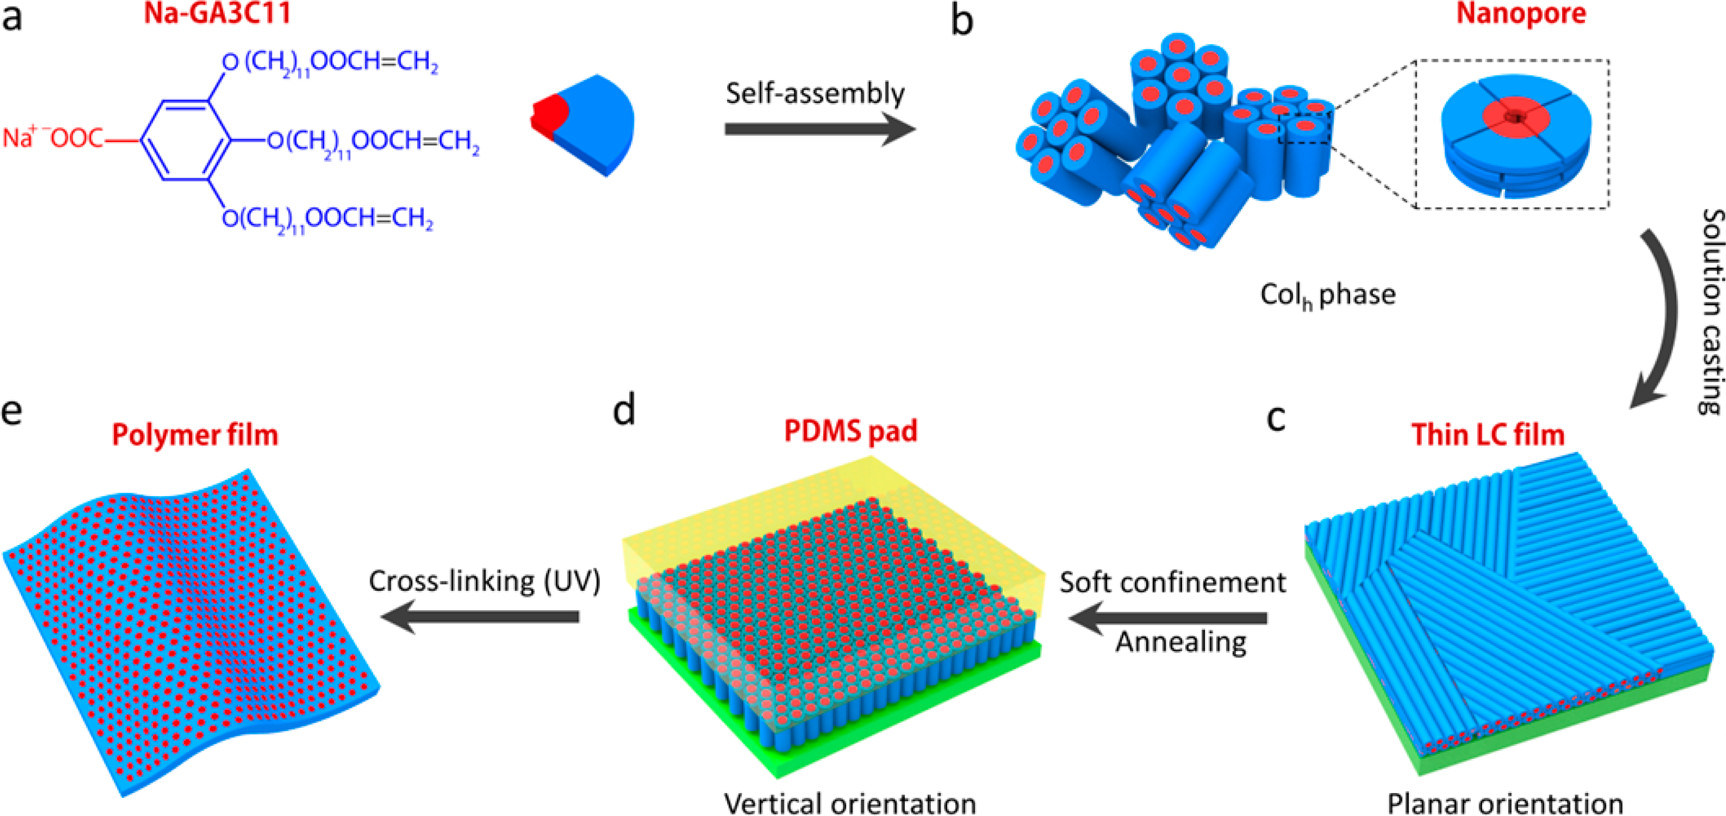
\includegraphics[width=\linewidth]{soft_confinement.png} \caption{The wedge
  %	  shaped liquid crystal monomer (a) self assembles into mesophases with
%		  hexagonally packed pores (b). The pores are made of stacked monomer disks. A
%		  sub-micron-thick film is created by casting a dilute solution of Na-GA3C11/THF
%		  solution onto a silicon substrate and and allowing the solvent to evaporate.
%		  The thin film contains nanoporous columns which lie parallel to the film plane.
%		  (d) When a soft PDMS pad is imposed to the thin film, with subsequent thermal
%		  annealing, the columns align perpendicular to the film plane. (e)
%		  Photo-cross-linking of the aligned film creates a mechanically stable thin film
%		  with vertically aligned nanopores}~\label{fig:soft} \end{figure}

  %BJC: Made my own version of the above, leaving out alignment details since it'

  %BJC: TODO: Scalable vector graphic for monomer structure, make bigger. Convert .svg to .eps
  %           Thicken slabs
  %           Make pore region on slab (blue) bigger
  %           Bump up atom sizes in atomistic render
  \begin{figure}
	\centering
	\begin{subfigure}{.3\textwidth}
		\centering
		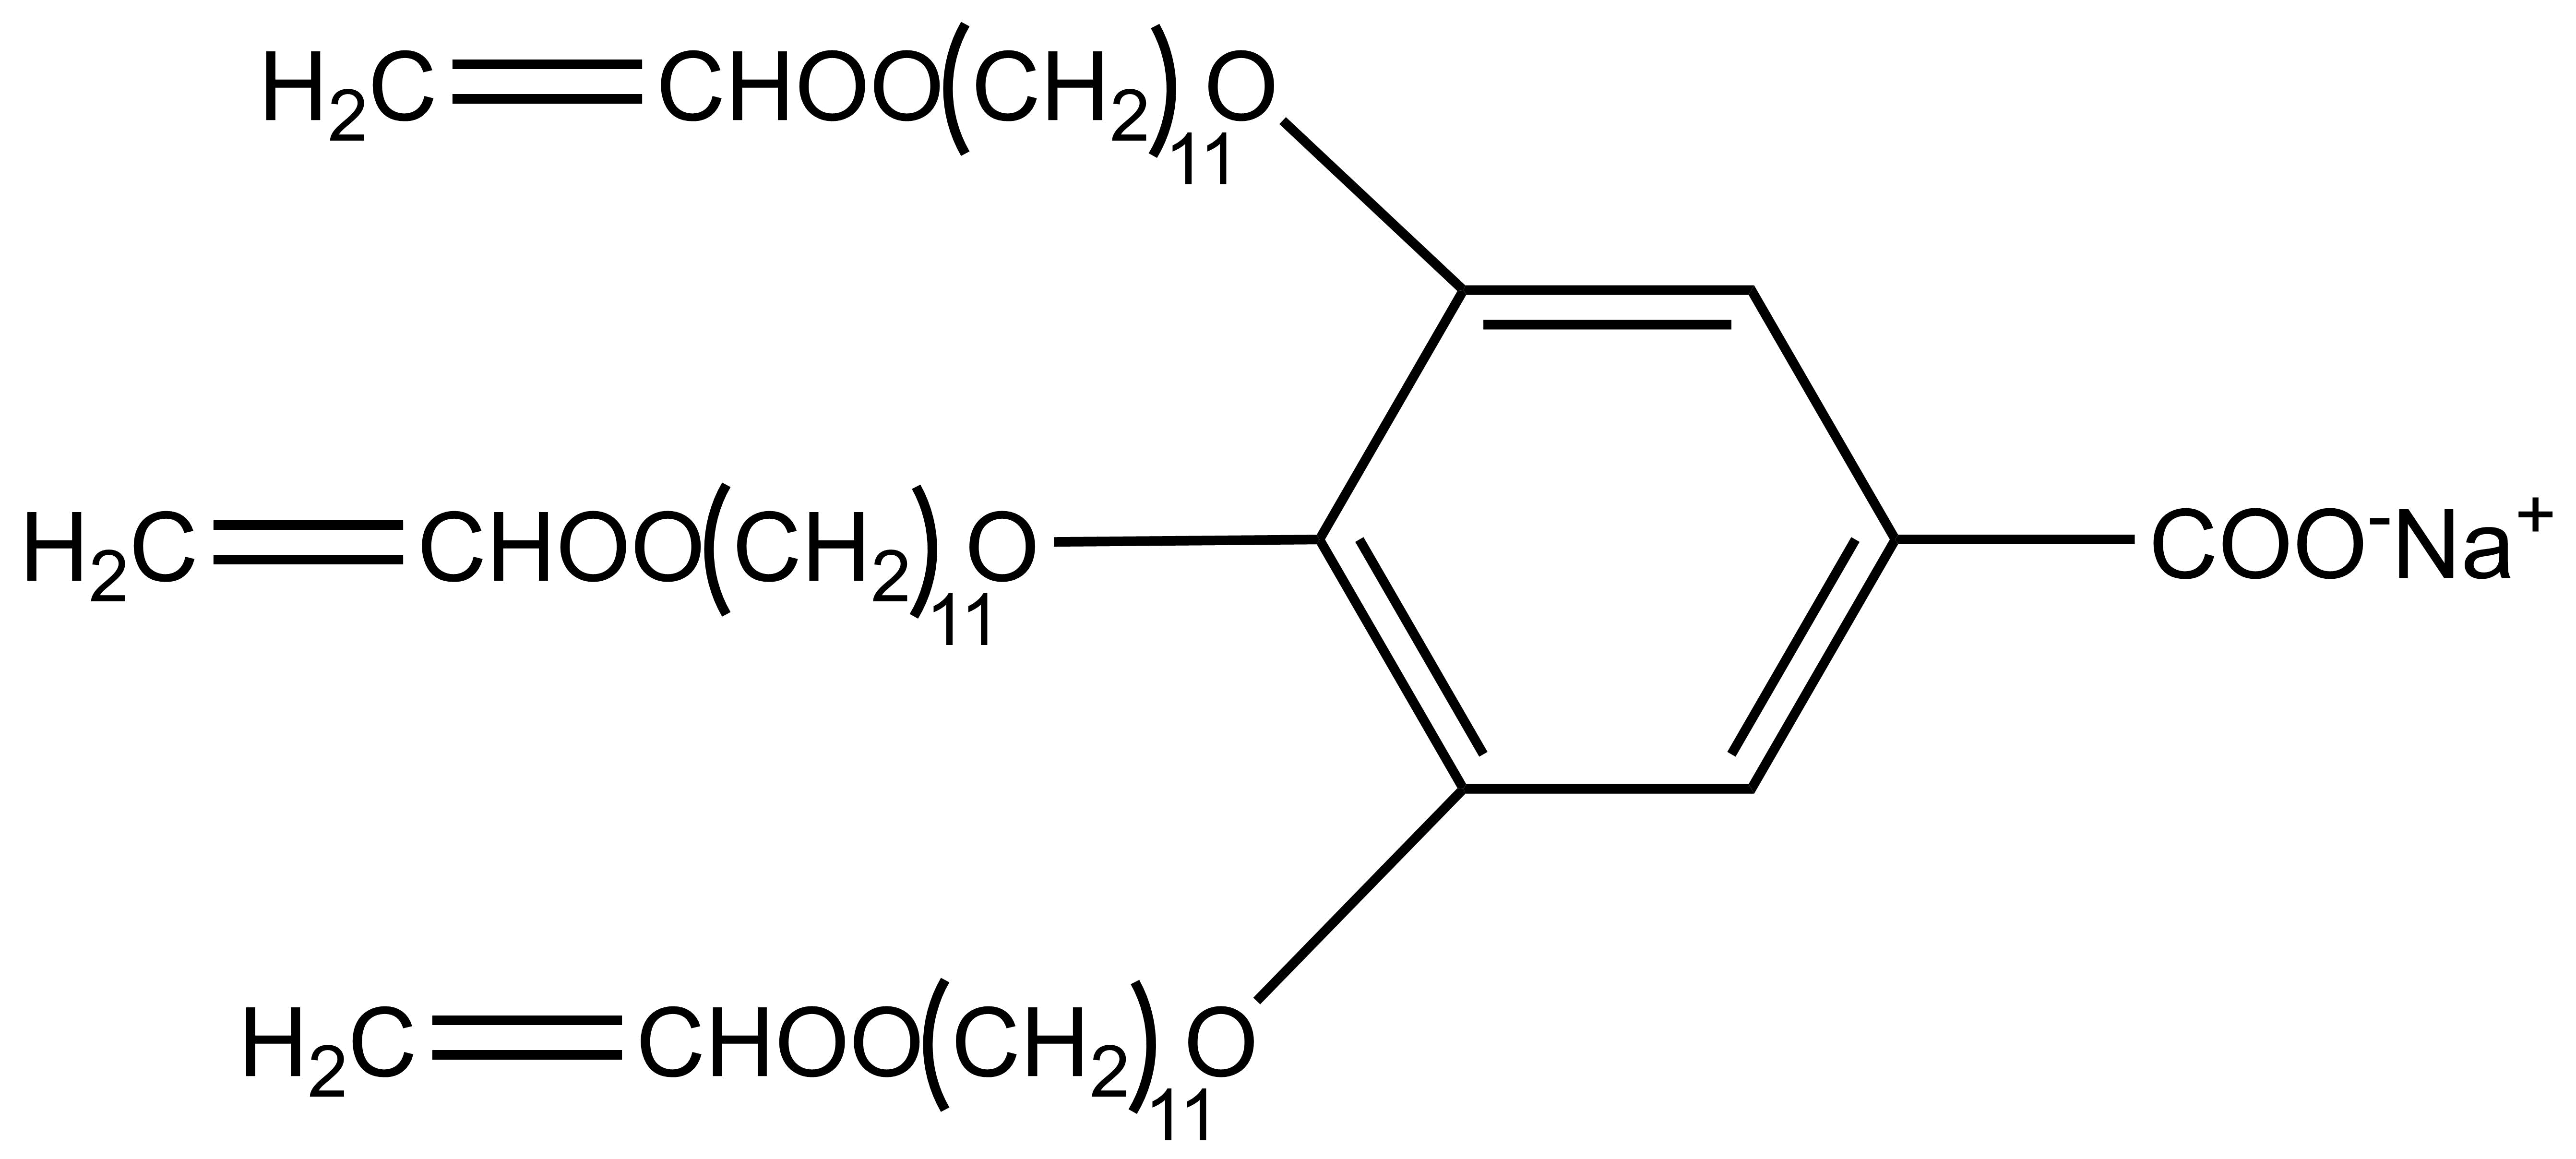
\includegraphics[width=\textwidth]{NaGA3C11.png}
		\caption{}~\label{fig:monomer}
	\end{subfigure}
	\begin{subfigure}{.3\textwidth}
		\centering
		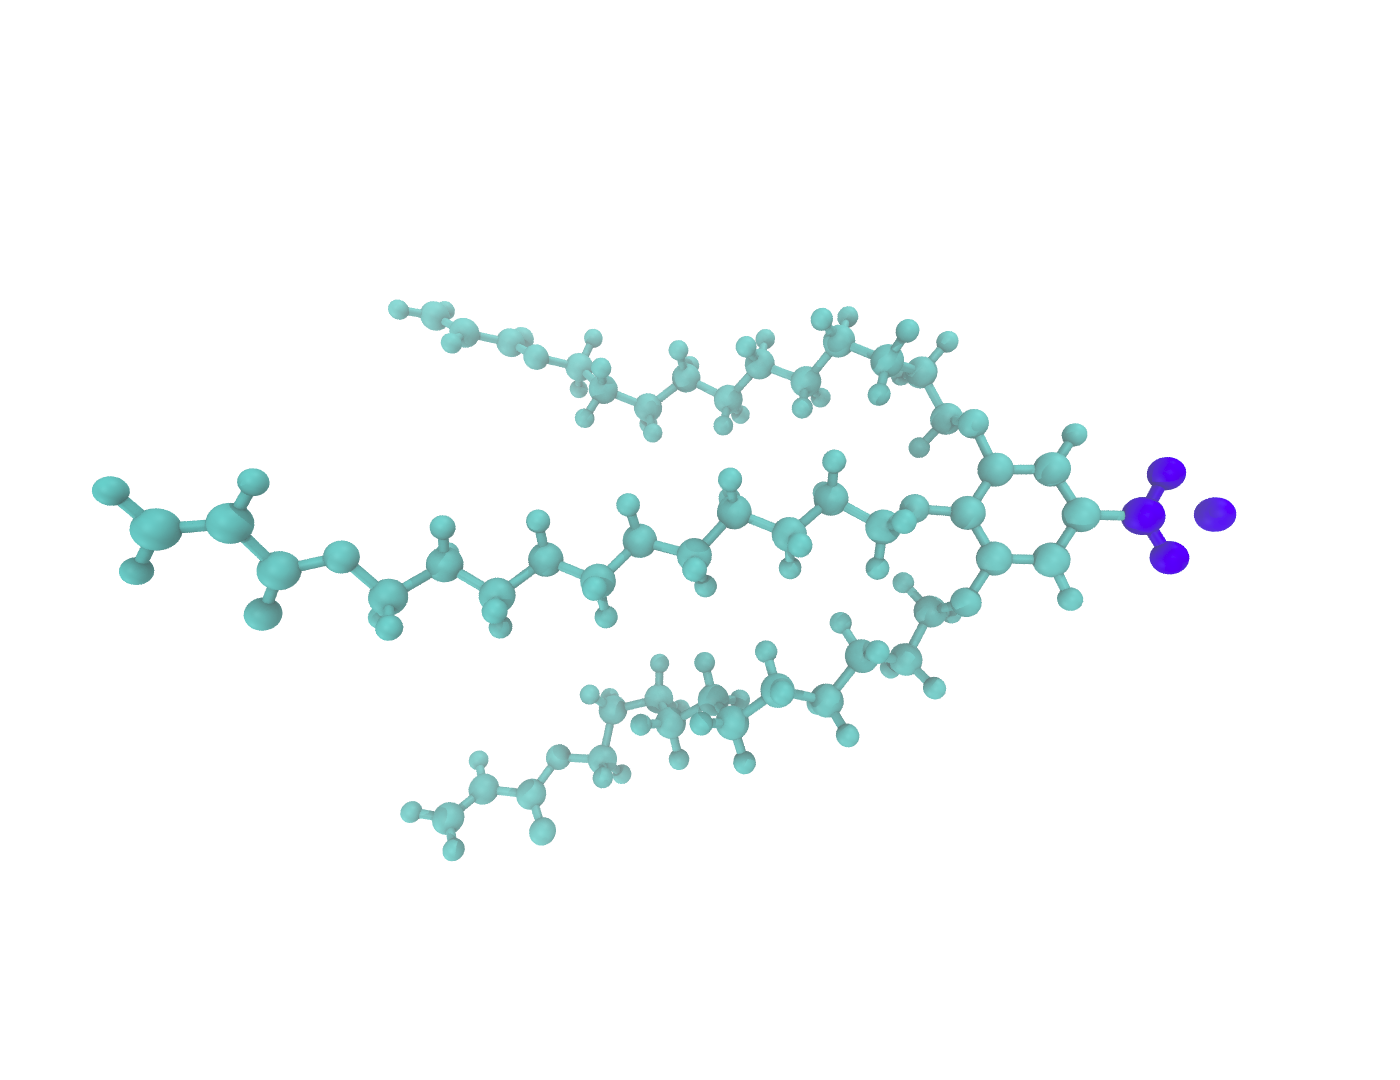
\includegraphics[width=\textwidth]{monomer_twocolor.png}
		\caption{}~\label{fig:atomistic_monomer}
	\end{subfigure}
	\begin{subfigure}{0.3\linewidth}
		\centering
		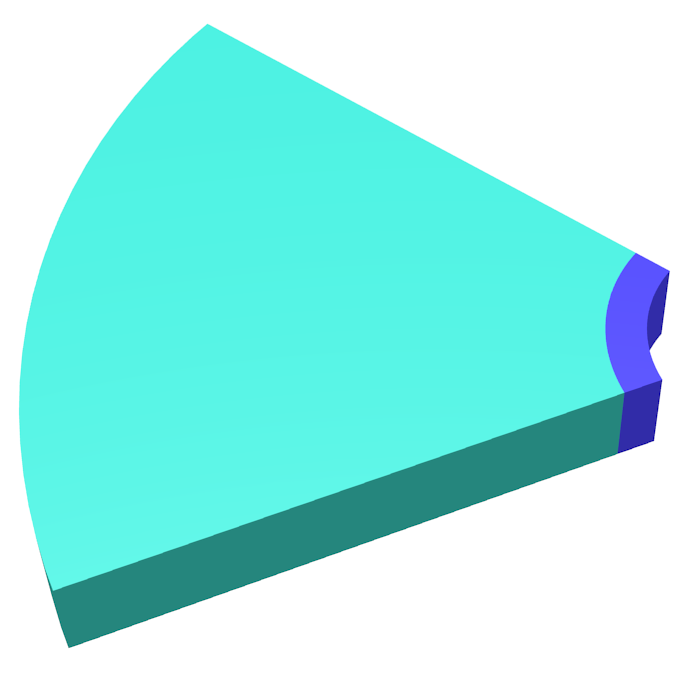
\includegraphics[width=\textwidth]{wedge.png}
		\caption{}~\label{fig:wedge}
	\end{subfigure}
		\begin{subfigure}{0.4\linewidth}
		\centering
		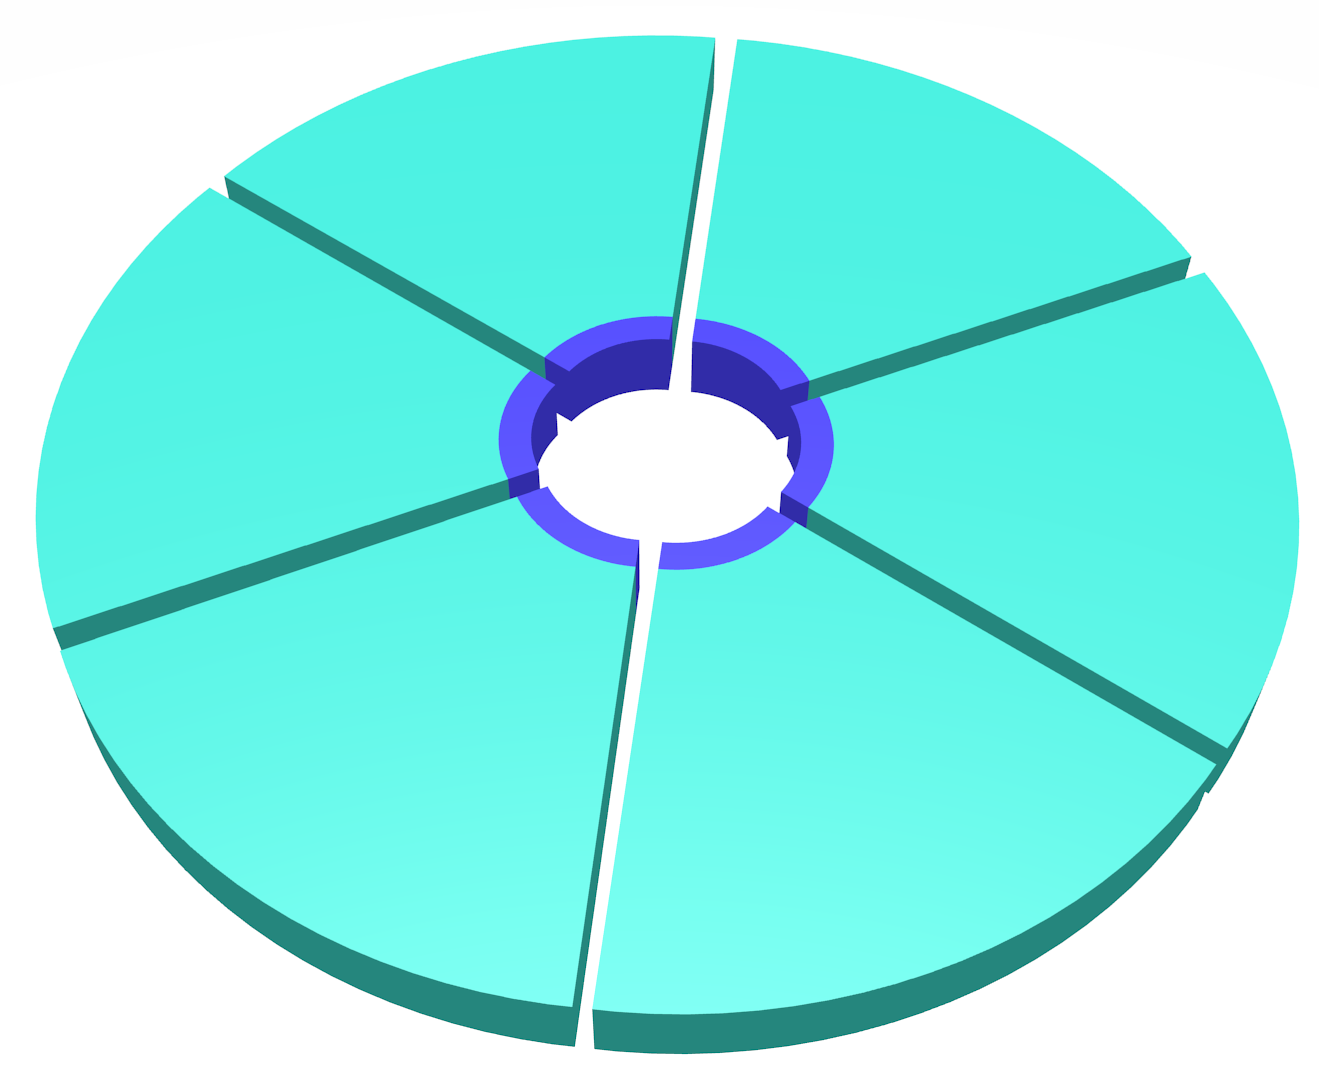
\includegraphics[width=\textwidth]{layer_blender.png}
		\caption{}~\label{fig:wedge_layer}
	\end{subfigure}
	\begin{subfigure}{0.4\linewidth}
		\centering
		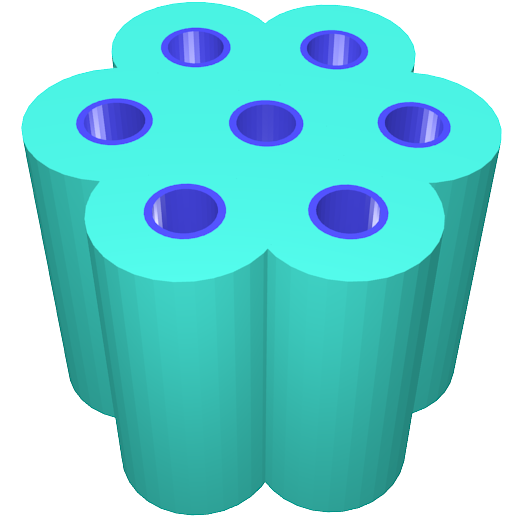
\includegraphics[width=\textwidth]{hexagonal_packing.png}
		\caption{}~\label{fig:hex_packing_simple}
	\end{subfigure}
	\caption{The liquid crystal monomer Na-GA3C11 (a) rendered atomistically (b)
	exhibits wedge-like character (c). Monomer wedges assemble into disks (d) with
	hydrophilic head groups (blue) facing towards the disk center. The disks
	assemble into hexagonally packed columnnar mesophases (e)}~\label{fig:assembly}
  \end{figure}

  Our current understanding of LLC systems is not rich enough to be able to
  precisely design membranes for specific separations. Over the past 20 years,
  H\textsubscript{II} phase LLC membrane studies have been limited primarily to
  Na-GA3C11 with some characterization done after minor structural modifications.
  Resel et al. varied the length of the monomer tails and the counterion used and
  observed its affect on pore spacing \cite{resel_structural_2000}.  Their study
  offers no insight into dynamics within the pore. In a later study of rejection
  performance, it was shown that membranes formed by Na-GA3C11 can not perform
  separations of solutes less than 1.2 nm in diameter because the pores are too
  large \cite{zhou_supported_2005}.  We do not yet understand how to controllably
  reduce the effective pore size or how to tune the chemical environment in the
  nanopores for effective water desalination and small organic molecule
  separations. The only source of predictive modeling for LLC systems have been
  macroscopic models which likely do not adequately describe transport at these
  length scales \cite{hatakeyama_water_2011}. It will be challenging to
  efficiently narrow down the large design space in a laboratory setting without
  a robust model.

  A molecular level understanding of LLC membrane structure, enabled by
  molecular dynamics simulations, will provide guidelines to reduce the large
  chemical space available to design monomers for creation of separation-specific
  membranes. A good molecular model should incorporate a detailed picture of the
  nanoscopic pore structure which will be crucial to understanding the role of
  monomer structure in solute transport and membrane design. Models resulting
  from molecular dynamics simulations will provide the required level of detail (Fig. \ref{fig:detail}).
  We can directly observe solute transport and suggest governing mechanisms. We
  can observe how the choice of head group may influence pore size for size
  exclusion driven separations. We can interchange counterions which may
  influence both the pore size and the strength of the Donnan potential which
  affects the degree to which the membrane can exclude charged species. 

  % BJC: TODO: Make new rendering of wedges
  %            Change color scheme 
  \begin{figure}
  \centering
	\begin{subfigure}{0.45\linewidth}
		\centering
		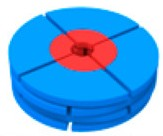
\includegraphics[width=\textwidth]{nanopore_undetailed.jpg}
		\caption{}~\label{fig:undetailed_pore}
	\end{subfigure}
	\begin{subfigure}{0.45\linewidth}
		\centering
		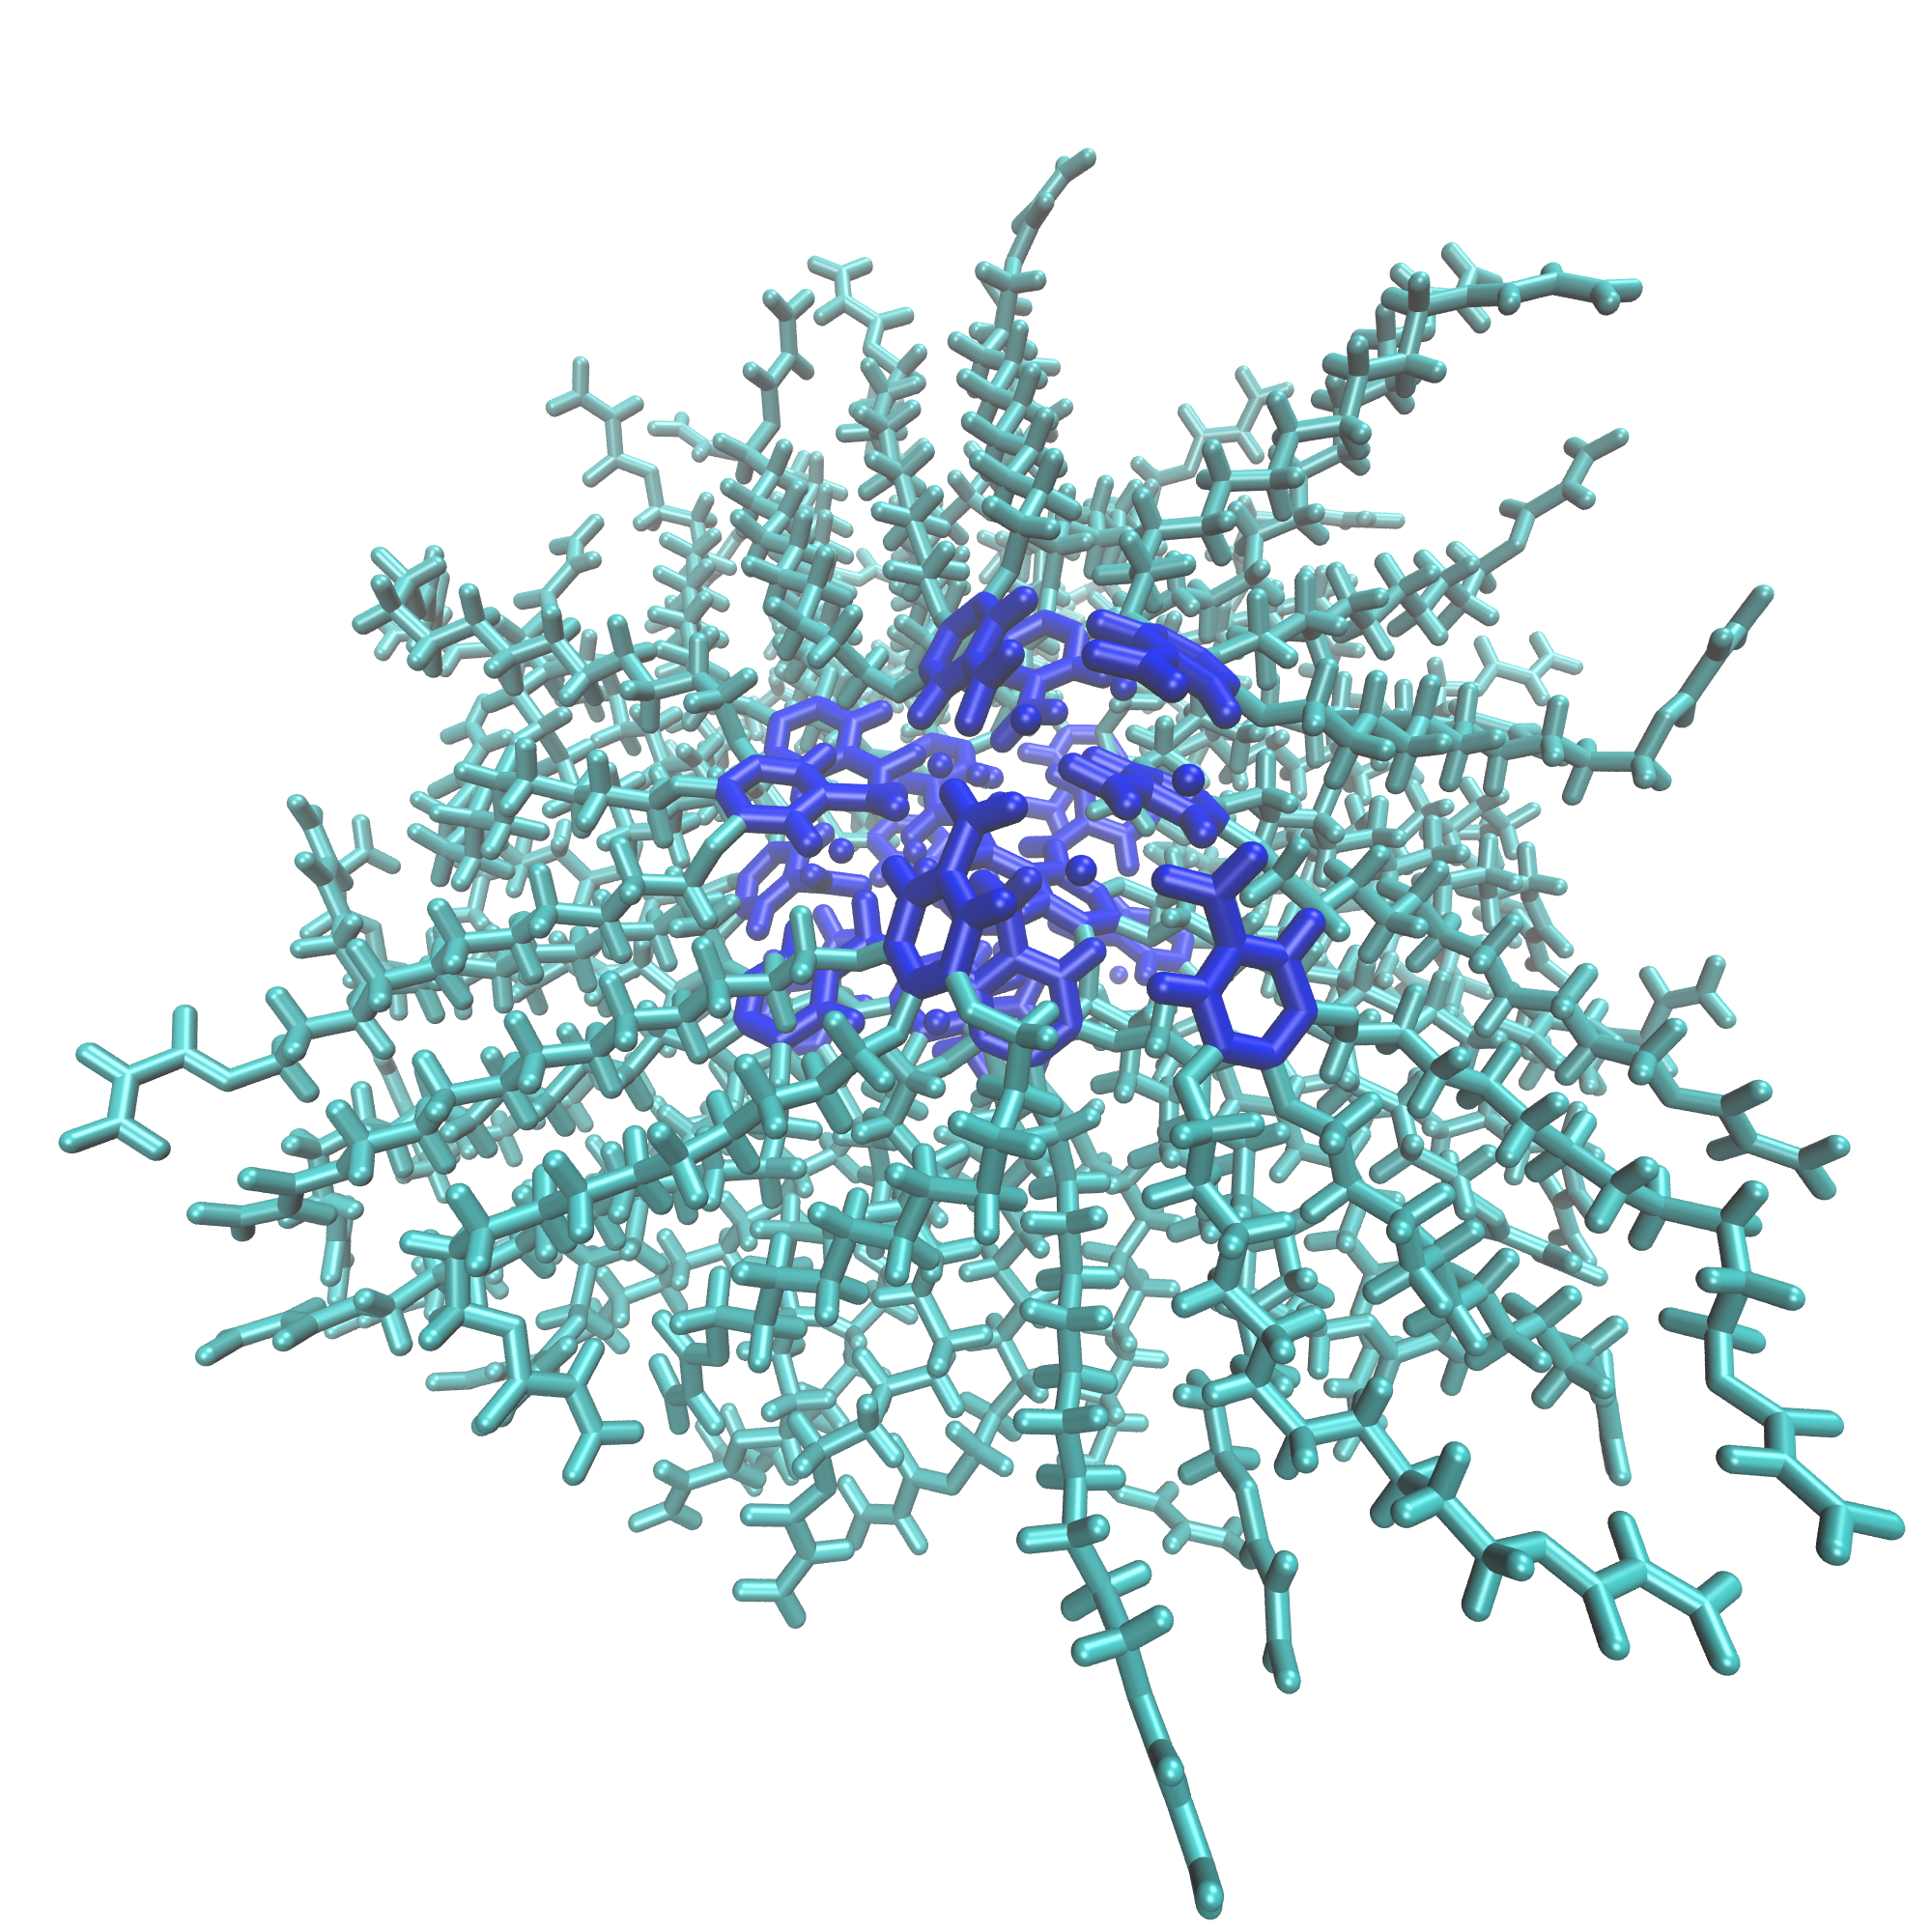
\includegraphics[width=\textwidth]{detailed_pore.png}
		\caption{}~\label{fig:detailed_pore}
	\end{subfigure}
  \caption{(a) Our previous understanding of the pore structure allows us to speculate
	   about separation behavior. (b) A detailed molecular model will allow us to
	   directly observe solute transport. Here, four stacked layers of 5 monomers
           are pictured atomistically. The hydrophilic region is in red and the 
	   hydrophoic region is colored blue.}~\label{fig:detail}
  \end{figure}
 
  %BJC: I think the first sentence of the following paragraph is
  %necessary to put somewhere, but maybe not in this spot exactly
  In order to appropriately model transport, we must first gain a thorough
  understanding of the nanoscopic structure of LLC membranes. Our approach to
  constructing a general model will follow the development of a model of the
  assembly formed by Na-GA3C11 since it has sufficient experimental
  characterization. We have also narrowed our scope to the development of a model
  of the Col\textsubscript{h} phase membrane. Compared to the H\textsubscript{II}
  phase, the Col\textsubscript{h} phase is a simpler starting point, due to the
  absence of water, and has detailed experimental wide-angle X-ray scattering
  (WAXS) patterns useful for reconstructing structural data.  

  Despite having structural data, there is still information which experiment
  cannot definitively answer. There are several key questions that we will
  investigate.
% which will be laid out and numbered in subsequent paragraphs.

  %BJC: commenting out :There has been no definitive answer in literature
  %regarding the number of monomers in each layer.  MRS3: the intro to the list
  %talks about only ``numbers of monomers in each layer'', whereas the list
  %below talks about several questions relating to layers. Can you rephrase so
  %it's more general? Maybe just take out that sentence above.

  Monomers in the Col\textsubscript{h} system are theorized to be partitioned
  into stacked layers which form columnar pores. We want to know 

  \begin{enumerate}

  \item If layers do exist, how many monomers constitute a single layer? \label{point:monomernum}
  
  A simple molecular simulation study of a similar molecule suggested that
  there are 4 monomers in each layer. Their estimation is based on a simulated
  system containing only 16 total monomers which likely does not sufficiently
  model the chemical environment present in the real system
  \cite{zhu_methacrylated_2006}.  A separate calculation based on the volume of
  the liquid crystal monomers proposes that there are seven monomers in each
  layer \cite{resel_structural_2000}.  A molecular model orders of magnitude
  larger than any other reported atomistic liquid crystal membrane simulations
  has the best chance of directly answering this question.  We will directly
  change the layer composition and note its effect on membrane structure.

 \item Does our model support the existence of layers and if so, how well
 defined are the layers? \label{point:layers} 

  Experimentally, their existence is supported by evidence of strong $\pi$-$\pi$
  stacking interactions in the direction perpendicular to the membrane plane.
  $\pi$-$\pi$ stacking will only occur between the aromatic monomer head groups
  which leaves no description of what is happening in the monomer tail region.
  The tails may entangle isotropically while stacking order is maintained among
  headgroups. 

  \item How do monomers in each layer position themselves with respect to
  surrounding layers? \label{point:orientation}

  The $\pi$-$\pi$ stacking interactions may be a driving force of self assembly
  in this system \cite{gazit_possible_2002}. Gas phase ab initio studies of
  benzene dimers have shown a clear energetic advantage for parallel displaced
  and T-shaped $\pi$-$\pi$ stacking conformations versus a sandwiched
  conformation ~\cite{sinnokrot_estimates_2002}. Substituted benzene rings
  exhibit an even stronger $\pi$-$\pi$ stacking attraction which favors the
  parallel displaced configuration in all cases except where the substitutions
  are extremely electron withdrawing.
  \cite{waller_hybrid_2006,ringer_effect_2006}. We will compare simulated X-ray
  diffration patterns to experiment in order to deduce which stacking 
  configurations is most likely. 

  \item Can the system exist in other metastable states or phases that are not
  accessed during experiments? \label{point:metastable}
  
  There remains the possibility that there is more than one metastable state
  associated with a given LLC system. Simulating a membrane atomistically will
  require many atoms which limits the timescales acessible with MD. It is
  reasonable to expect that we will generate configurations which are kinetically
  trapped in a metastable free energy basin. We must be able to identify which
  state is produced experimentally.

  \item What constitutes a pore and how well-defined are the pore regions? \label{point:poredefinition}

  The limited picture that experiment provides tells us that there are
  hexagonally packed, hydrophilic regions where transport is likely to occur.
  One may instinctively assume that these regions are tube-like pathways. We will
  explore the composition of the pores and the partition between the
  hydrophilic and hydrophobic regions. 

  \item Is it necessary to include any water in order to appropriately model
  the Col\textsubscript{h} phase? \label{point:water}

  While the Col\textsubscript{h} phase is described as dry, it has been
  suggested by experimentalists, in unpublished communications, that it is likely
  that small amounts of ambient water are leached into neat monomer.
  Experimentally, achieving a hexagonal phase with a completely dry system has
  proven difficult. If neat monomer is allowed to sit in ambient conditions, its
  color turns from transparent to slightly opaque and a hexagonal phase forms.
  Although we will not explore whether water is necessary for self assembly, we
  hypothesize that the hydrogen bonding network formed by the water may play a
  role in structuring the pores and holding together the hexagonal phase. We can
  use simulated X-ray diffraction patterns to see if there is any meaningful
  structural difference between a "dry" and "wet" system.

  \end{enumerate}
  
  %Once we have addressed all of the above questions, we must show that the 
  %developed molecular model is consistent with physical observations so that we
  %can rely on conclusions drawn about structural features characteristic of 
  %the system.
 
  %BJC: Would it be better to describe each reflection as a numbered list (like with the questions above?)
  We used experimental small-angle X-ray scattering (SAXS) data from
  \cite{feng_thin_2016} (Fig. ~\ref{fig:SAXS}) and wide angle X-ray scattering
  (WAXS) data (Fig. ~\ref{fig:WAXS}, produced as described in
  \cite{feng_scalable_2014}) for comparison to our model. We rely primarily on the 2D WAXS data
  since it encodes all structural details down to the sub-nm scale.  There are
  five major features of interest present in the 2D experimental pattern shown in
  Figure \ref{fig:WAXS}. The first is located at $q_z$ = 1.7 \angstrom$^{-1}$,
  corresponding to a real space separation of 3.7 \angstrom~.  The reflection is
  attributed to $\pi$-$\pi$ stacking between aromatic rings in the direction
  perpendicular to the membrane plane, or z-axis \cite{feng_scalable_2014}. For
  simplicity, this reflection will be referred to as R-$\pi$. A weak intensity
  line is located at exactly half the $q_z$ value of R-$\pi$ ($q_z$ = 0.85
  \angstrom$^{-1}$), corresponding to a real space periodic spacing of 7.4
  \angstrom~. This reflection has been interpreted as 2\textsubscript{1} helical
  ordering of aromatic rings along the z axis meaning if the positions of the
  aromatic rings can be traced by a helix, then for each full turn in the helix, one
  will encounter two aromatic rings. For this reason it will be referred to as
  R-helix. A third major reflection is marked by a low intensity ring located at
  r = 1.4 \angstrom$^{-1}$. The real space separation corresponds to 4.5 \angstrom~
  which is characteristic of the average spacing between packed alkane chains.
  This reflection will be called R-alkanes. Within R-alkanes, are four spots of
  higher relative intensity which will be called R-spots. All are located
  $\approx 37$ degrees from the $q_z$ axis in their respective quadrants. In many
  liquid crystal systems this can be explained by the tilt angle of the alkane
  chains with respect to the membrane plane. The final feature corresponds to the
  spacing and symmetry of the d\textsubscript{100} plane which can be related to
  the distance between pores.  The feature, which will be called R-pores, is
  characterized by dots along $q_z$ = 0. The spacing between dots is indicative
  of the hexagonal symmetry of the packed pores. The same information at higher
  resolution is obtained using a SAXS setup. 

  In this study, we build a significantly more realistic atomistic model of LLC
  membranes than, to our knowledge, has ever previously been done, and explore
  what new structural information can be gained and what structure hypotheses are
  supported by this model. We validate the model using as much experimental
  information as possible. We are most interested in reproducing the conclusions
  about structure which have been drawn from X-ray diffraction (XRD) experiments
  and in matching ionic conductivity measurements \cite{feng_thin_2016}.

  %BJC: TODO: update colorbar
  \begin{figure}
        \centering
        \begin{subfigure}[t]{0.43\linewidth}
                \centering
                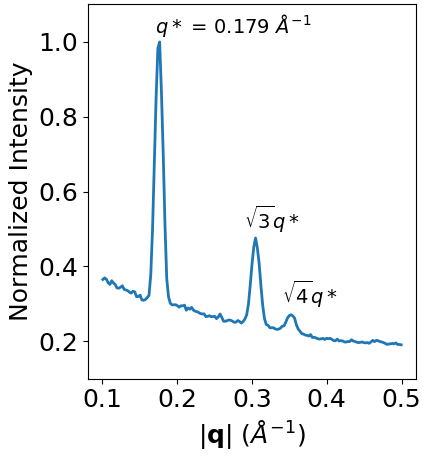
\includegraphics[width=\linewidth]{SAXS.png}
                \caption{}\label{fig:SAXS}
        \end{subfigure}
        \begin{subfigure}[t]{0.47\linewidth}
                \centering
                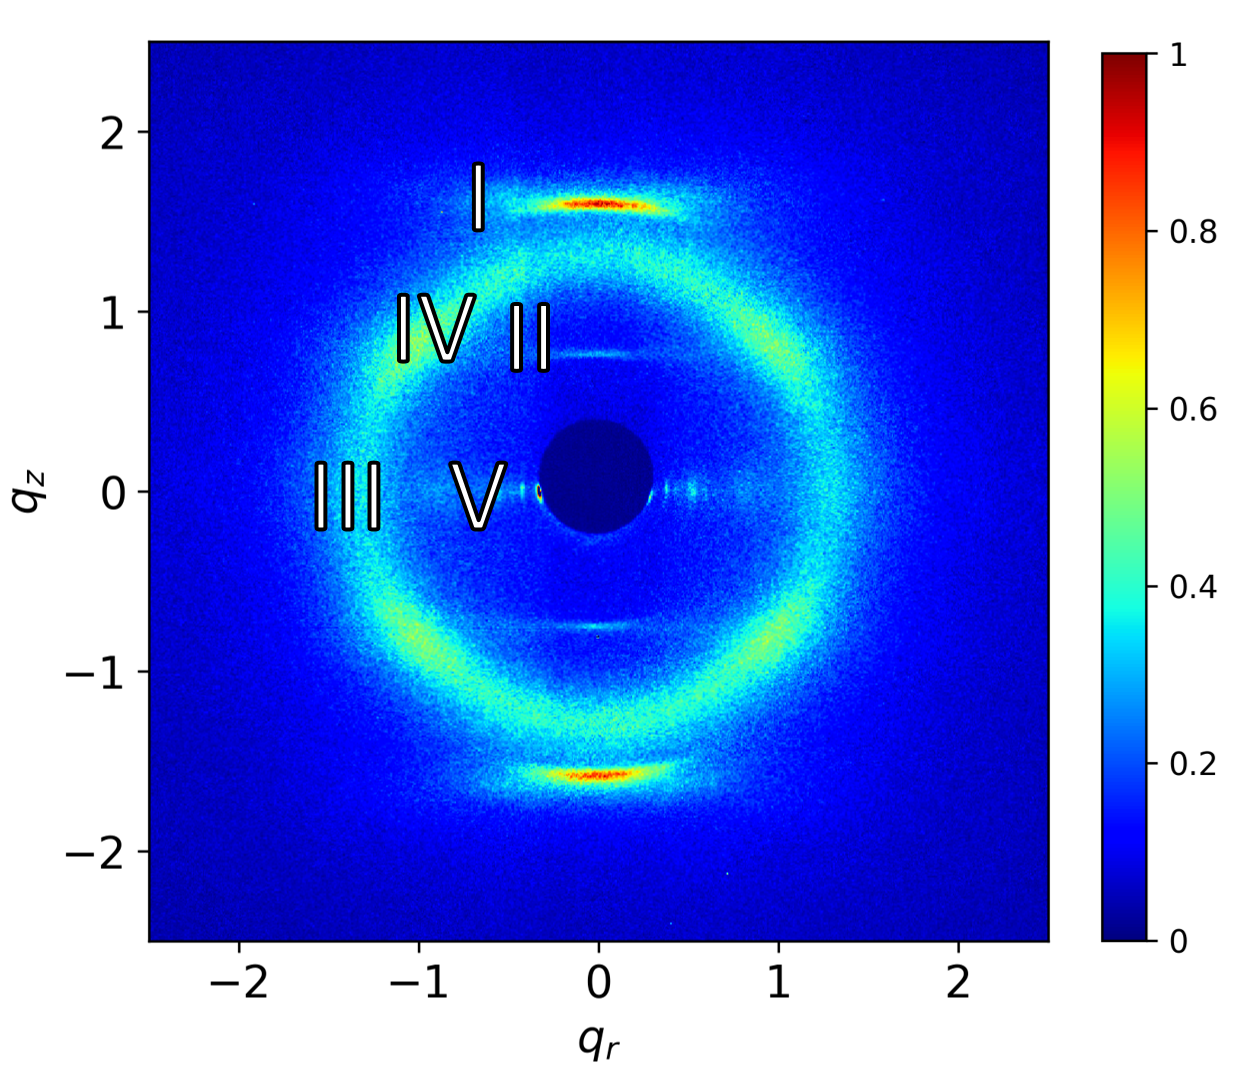
\includegraphics[width=\linewidth]{WAXS_annotated.png} 
                \caption{}\label{fig:WAXS}
        \end{subfigure}
	\caption{(a) The repeat spacing in the 1D small angle X-ray scattering pattern
		is characteristic of hexagonal packing. The leading peak represents the
		distance between the d\textsubscript{100} planes. Using this distance, we know
		that the distance between pore centers is 4.12 nm. (b) 2D wide angle X-ray
		scattering gives details about repeating features less than 1 nanometer
		apart. Experimentalists have justified each of the 5 major reflections
		present as follows: (I) Aromatic head group $\pi-\pi$ stack 3.7 \AA~apart.
		(II) Monomers arrange vertically in a 2\textsubscript{1} helix. (III) Alkane
 		chain tails pack 4.5 \AA~apart. (IV) Monomer tails tilt with respect to the 
 		membrane plane. (V) As derived from SAXS, pores pack hexagonally and are 
		spaced 4.12 nm apart}
	\label{fig:SWAXS}
 \end{figure}

  \section{Methods}
 
  \subsection{Monomer Parameterization}

  Liquid crystal monomers were parameterized using the Generalized AMBER
  Forcefield \cite{wang_development_2004} with the Antechamber package
  \cite{wang_automatic_2006} provided with AmberTools16
  \cite{case_ambertools16_2016}. Atomic charges were assigned using the am1bccsym
  method of molcharge shipped with QUACPAC from Openeye Scientific Software. All
  molecular dynamics simulations were run using Gromacs 2016.
  \cite{bekker_gromacs:_1993,berendsen_gromacs:_1995,van_der_spoel_gromacs:_2005,hess_gromacs_2008}

  An ensemble of characteristic, low-energy vacuum monomer configurations
  were constructed by applying a simulated annealing process to a parameterized
  monomer. Monomers were cooled from 1000K to 50K over 10 nanoseconds.  A low
  energy configuration was randomly pulled from the trajectory and charges were
  reassigned using molcharge.  Using the new charges, the monomer system was
  annealed again and a random monomer configuration was pulled from the
  trajectory to be used for full system construction (Figure~\ref{fig:python}a).

  \subsection{Unit Cell Preparation}

  The timescale for self assembly of monomers into the hexagonal phase is
  unknown and likely outside of a reasonable length for an atomistic simulation,
  calling for a more efficient way to build the system.  Previous work has shown
  a coarse grain model self assemble into the H\textsubscript{II} phase
  configuration in $\approx$ 1000 ns \cite{mondal_self-assembly_2013}.  We
  attempted atomistic self-assembly by packing monomers into a box using Packmol
  \cite{martinez_packmol:_2009}.  Simulations of greater than 100 ns show no
  indicators of progress towards an ordered system To bypass the slow
  self-assembly process, python scripts are used to assemble monomers into a
  structure close to one of a number of hypothesized equilibrium configurations
  (Figure~\ref{fig:python}).

  %BJC: TODO: reproduce figure in latex (or gimp?) with higher resolution arrows
  \begin{figure}
	\centering
	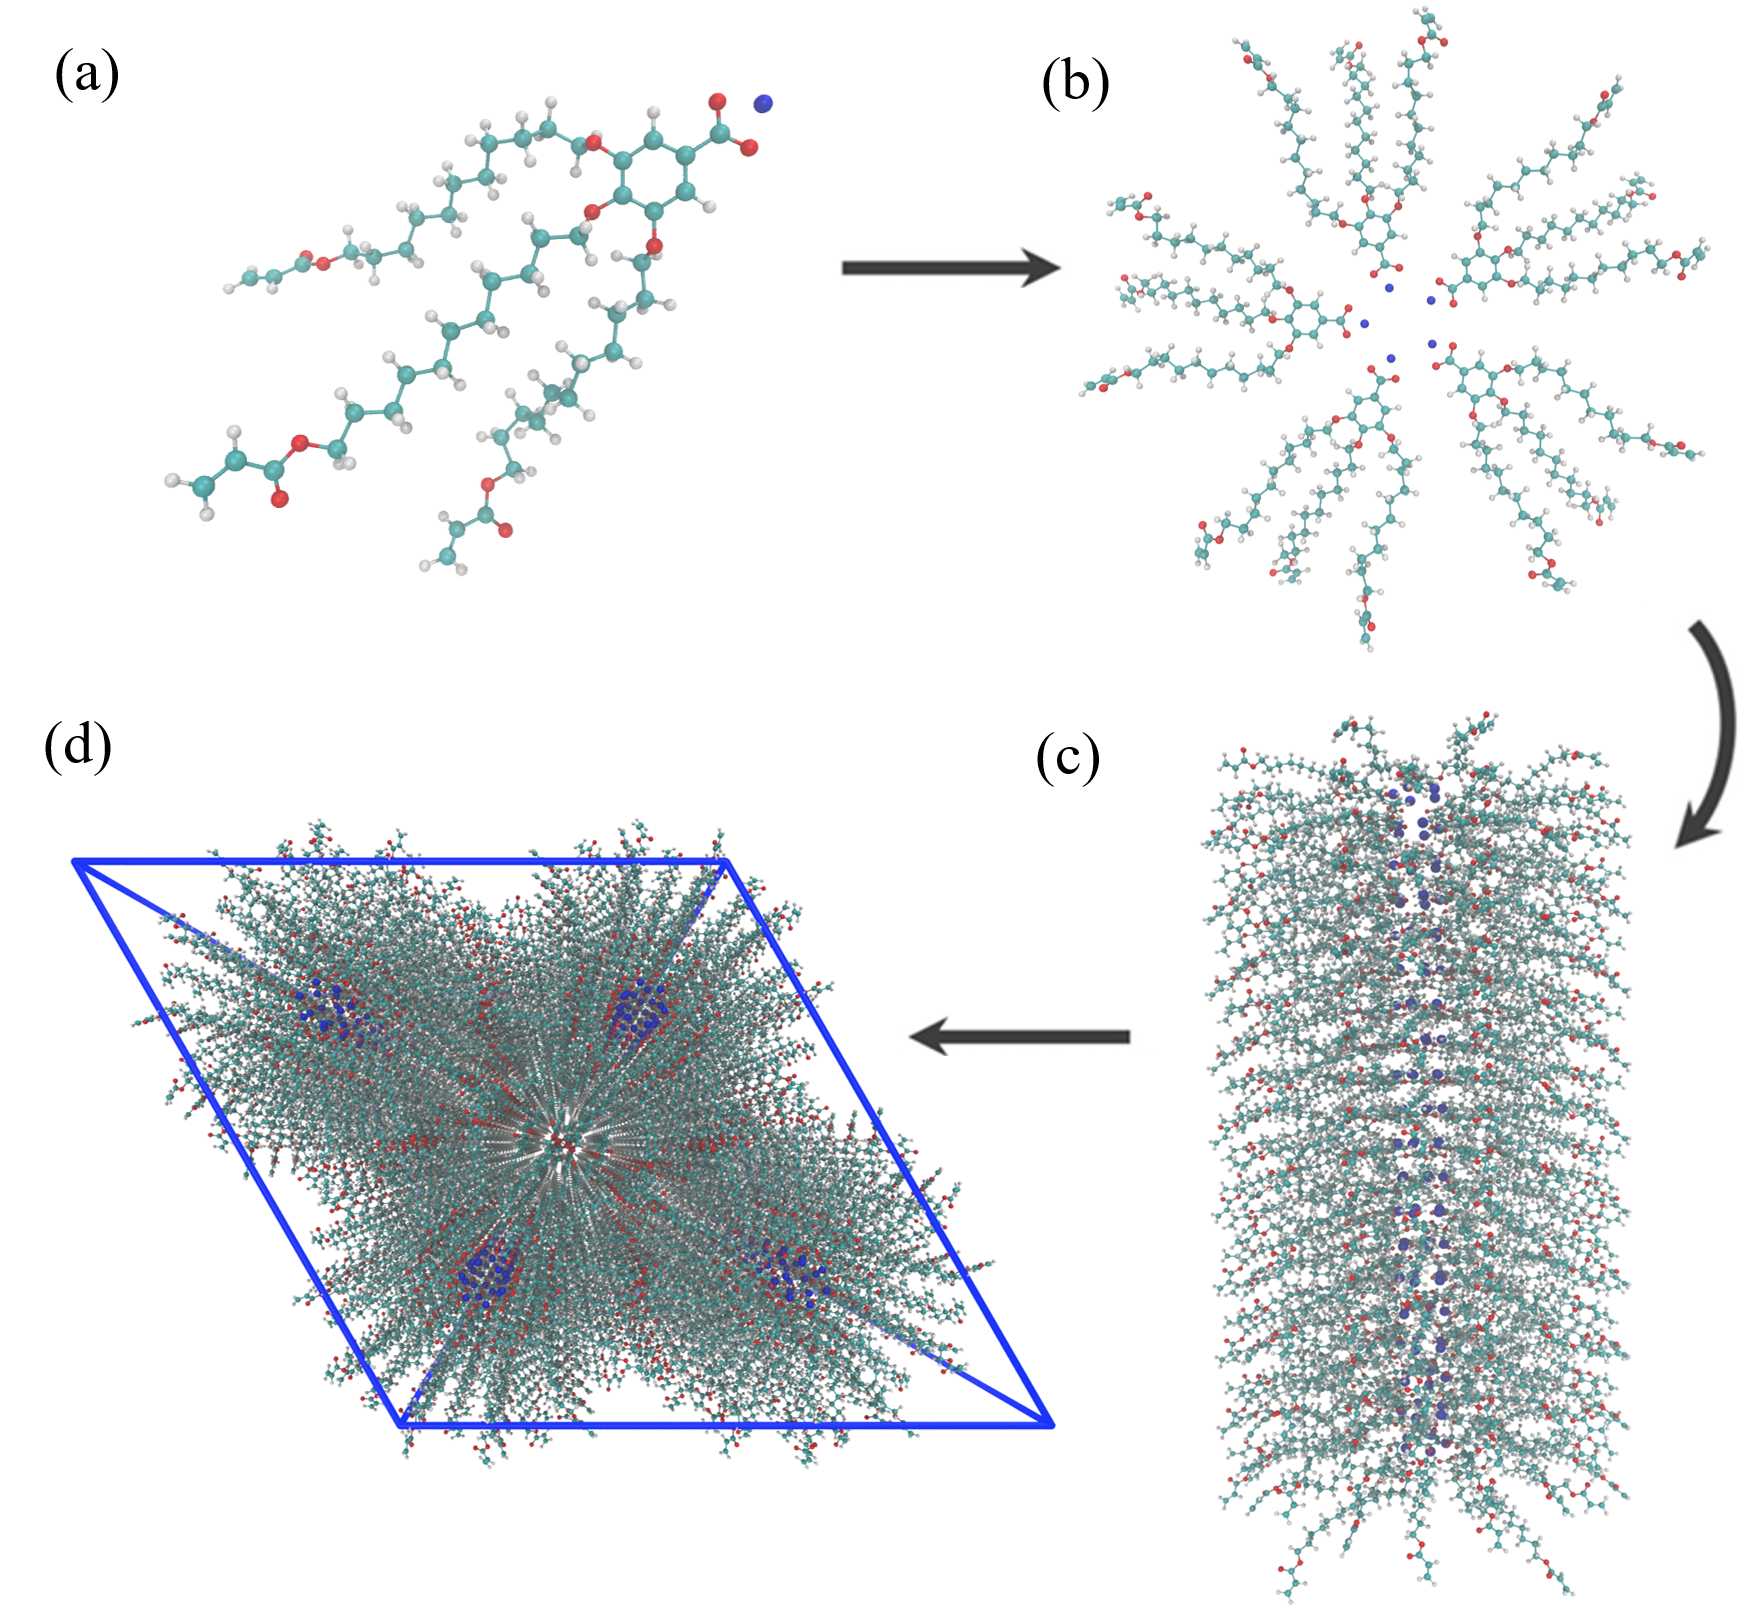
\includegraphics[width=0.75\linewidth]{build.PNG} %BJC: put an xyz axis with the unit cell
	\caption{(a) A single monomer was parameterized and annealed to produce a low energy
		configuration. (b) Monomers are rotated and assembled into layers with 
		hydrophlic centers. (c) Twenty layers are stacked on top of each other to create
		a pore. (d) Pores are duplicated and placed into a monoclinic unit cell}\label{fig:python}
  \end{figure}
  
  A typical simulation volume contains four pores in a monoclinic unit cell,
  the smallest unit cell that maintains hexagonal symmetry when extended
  periodically. Each pore is made of twenty stacked monomer layers with periodic
  continuity in the z direction, avoiding any edge effects and creating an
  infinite length pore ideal for studying transport. A small number of layers is
  preferred in order to reduce computational cost and to allow us to look at
  longer timescales. Ultimately, we chose to build a system with 20 monomer
  layers in each pore in order to obtain sufficient resolution when simulating
  X-ray diffraction patterns. %This point will be explained in more detail later.

\subsection{Monomer Placement} 

  When constructing an initial configuration, there are a number of variables
  which require careful consideration while placing monomers. The equilibrium
  configuration is sensitive to some while insensitive to others. The starting
  pore radius, defined as the distance of a chosen head group carbon from the
  pore's central axis, does not influence the equilibrium structure when a
  reasonable value is chosen (See Supplemental). The pore radius is chosen to be
  0.6 nm in our initial configurations because the pore size is estimated to be
  $\approx$ 1.2 nm. The initial distance between pores also has little effect on
  the the equilibrated structure. However, one should not start them too close or
  there will be high energy repulsions during early equilibration. We chose an
  initial pore spacing of 4.5 nm, $\approx$ 10 \% larger than the experimental
  value of 4.12 nm.  The distance between layers, the rotation of the layers with
  respect to adjacent layers, and the number of monomers per layer do influence
  the equilibrium structure and require further justification for their choices.
  We rely on experimental data to inform them. 

  We chose the layer spacing for the initial configuration based on R-$\pi$ and
  then allowed the system to readjust during equilibration. Each monomer was rotated
  so the plane of the aromatic head groups would be coplanar with the xy plane.
  We explore two different initial layer spacings. The first is exactly equal to
  R-$\pi$ with layers placed so aromatic rings are stacked 3.7 \angstrom~ apart
  in the z-direction. A second system is explored with an initial layer spacing
  of 5 \angstrom. A third system with an initial layer spacing of 10 \angstrom was
  briefly explored. When layers are spaced out too far, they will collapse
  on each other while simultaneously slipping in between layers of adjacent pores
  which leads to an artificially thick membrane with pores spaced closely
  together. There will be no further discussion of this system but the interested
  reader can learn more about it in the supplemental information.

  The relative interlayer orientation was chosen based on clues from
  diffraction data as well as the various known stacking modes of benzene and
  substituted benzene rings: sandwiched, parallel-displaced and T-shaped
  ~\cite{sinnokrot_estimates_2002} (\Cref{fig:sandwiched,fig:pd,fig:tshaped}).
  The T-shaped configuration was ruled out because its $\approx$ 5 \angstrom~
  equilibrium stacking distance ~\cite{sinnokrot_estimates_2002} is inconsistent
  with R-$\pi$. It is also unfeasible for the monomers to orient in the T-shaped
  conformation because of the bulky tail groups. The system's preference towards
  the sandwiched vs. parallel displaced stacking modes will be explored in some
  detail.  Both have reported stacking distances near the R-$\pi$ value of 3.7
  \angstrom. Headgroups in our sandwiched initial configuration are stacked
  directly on top of each other while stacked headgroups in the parallel
  displaced initial configuration are offset by $180/nmon$ degrees where $nmon$
  equals the number of monomers per layer.

  As outlined in (\ref{point:monomernum}) the number of monomers in each layer is
  unknown. We tested configurations constructed with a varied number of
  monomers per layer. Systems were built in the offset and parallel displaced
  configurations with 4, 5, 6, 7 and 8 monomers per layer.

  \subsection{Equilibration}

  We developed equilibration schemes to create dry and wet configurations. Both
  schemes start with an initial configuration generated according to the previous
  guidelines. To create a dry configuration, we fix monomer head groups in the
  sandwiched or parallel-displaced configuration using position restraints with a
  force constant of 1e6 KJ mol$^{-1}$ nm$^{-2}$. We run a 50 ps simulation in the
  NVT ensemble which allows the monomer tails to settle without disrupting the
  ordering of the head groups. Doing so also mitigates system dependence on
  initial monomer configuration. Every 50 ps, we reduce the force constants by
  the square root of its previous value. Once the force constant is below 10 KJ
  mol$^{-1}$ nm$^{-2}$, the restraints are released linearly until there is no more
  restraining potential. The resulting unrestrained structure is allowed to
  equilibrate for 5 ns in the NPT ensemble with pressure controlled by the
  berendsen barostat. Next, we run long NPT equilibration simulations for at
  least 400 ns using the Parrinello-Rahman barostat with a time consant of 10 ps.

  In order to create a wet system, we solvated an initial configuration with
  water using gmx solvate. All water molecules placed outside the pore region are
  removed. Waters inside the pore region are randomly removed until the desired
  concentration of water in the pores is reached. The remainder of the
  equilibration follows the same procedure as the dry system. 

  \subsection{Crosslinking}
  
  % BJC: Need to make it clear that this was not done on all systems

  In order to fully match synthetic procedures, we created a crosslinking
  algorithm that can be applied to equilibrated structures. The purpose of 
  crosslinking
  is to maintain macroscopic alignment of the crystalline domains, 
  ensuring aligned, hexagonally packed pores. For that reason, we are not
  concerned with replicating the kinetics of the reaction, but instead emphasize
  the consistency of the final structure with experimental structural data. The
  algorithm was developed based on the known reaction mechanism. Crosslinking of
  this system is a free radical polymerization (FRP) taking place between
  terminal vinyl groups present on each of the three monomer tails. FRPs require
  an initiator which bonds to the system, meaning new atoms are introduced into
  the system. For simplicity, the initiator was simulated as hydrogen and made
  present in the simulation by including them in all possible locations where an 
  addition could occur as dummy atoms. The crosslinking procedure is carried out
  iteratively. During each iteration, bonding carbon atoms are chosen based on
  a distance cut-off. The topology is updated with new bonds and dummy hydrogen
  atoms are changed to appropriate hydrogen types. Head-to-tail addition was the
  only propagation mode considered due to its dominance in the real system.
  Direction of attack was not considered because the resultant mixture is
  racemic.

  Our implementation requires long simulation times to achieve high degrees
  of crosslinking. For that reason we did not crosslink all systems tested, but only the most
  promising structure. We show that crosslinking does not significantly 
  change any of our drawn conclusions in Section 3.6.

  \subsection{Equilibrium Calculations}

  Using equilibrated structures, we carry out various calculations to
  characterize the system. We define the point at which a system is
  equilibrated based on when the distance between pores stops changing.

  To calculate the equilibrated pore spacing, we measured the distance between
  pore centers. Pore centers are located by averaging the coordinates of sodium
  ions in their respective pores. Pore spacing statistics were generated 
  using the bootstrapping technique (See Supplemental Information).

  To quantify the degree of layering and the equilibrium distance between layers
  in our system, we calculate a spatial correlation function, $g(z)$, measured
  along the z-axis (perpendicular to the membrane plane). To calculate $g(z)$,
  we binned the z-component distances between the center of mass of each
  component and all others of the same pore over at least 50 ns of equilibrated
  trajectory and then normalized by the average number density. To extract the
  average distance between layers we applied a discrete fourier transform to
  $g(z)$ and extracted the highest intensity frequency.

  % BJC: To be replaced by Joe's description
  Simulated X-ray diffraction patterns are generated based on atomic
  coordinates in order to make a direct experimental comparison. All atomic
  coordinates were simulated as gaussian spheres of electron density
  corresponding to each atom's atomic number. A three dimensional fourier
  transform (FT) of the array of electron density results in a three dimensional
  structure factor which represents the unit cell in reciprocal space. We matched
  experimental 2D WAXS patterns by adjusting the initial spacing between layers
  and the orientation of the head groups with respect to adjacent layers.

  The colorbars on all diffraction patterns are normalized relative to
  R-alkanes. We calculated the average intensity within R-alkanes of the
  experimental pattern, $I_{avg}$.  We exclude intensities within $\pm$
  30\degree~of the $q_r=0$ axis, since the simulated patterns differ from
  experiment in those regions (See Fig. \ref{fig:XRDsim}).  We multiplied $I_{avg}$
  by a scaling factor of 2.5.  Intensities that appear in the experimental
  pattern $\geq$ 2.5$*I_{avg}$ receive colorbar values of 1. The result of this
  colorbar scaling method is shown in Figure \ref{fig:WAXS}. We apply the same
  scaling method to the simulated patterns.  

  % BJC: I think this figure belongs somewhere else
  \begin{figure}
	\centering
	\begin{subfigure}[b]{0.32\textwidth}
		\centering
		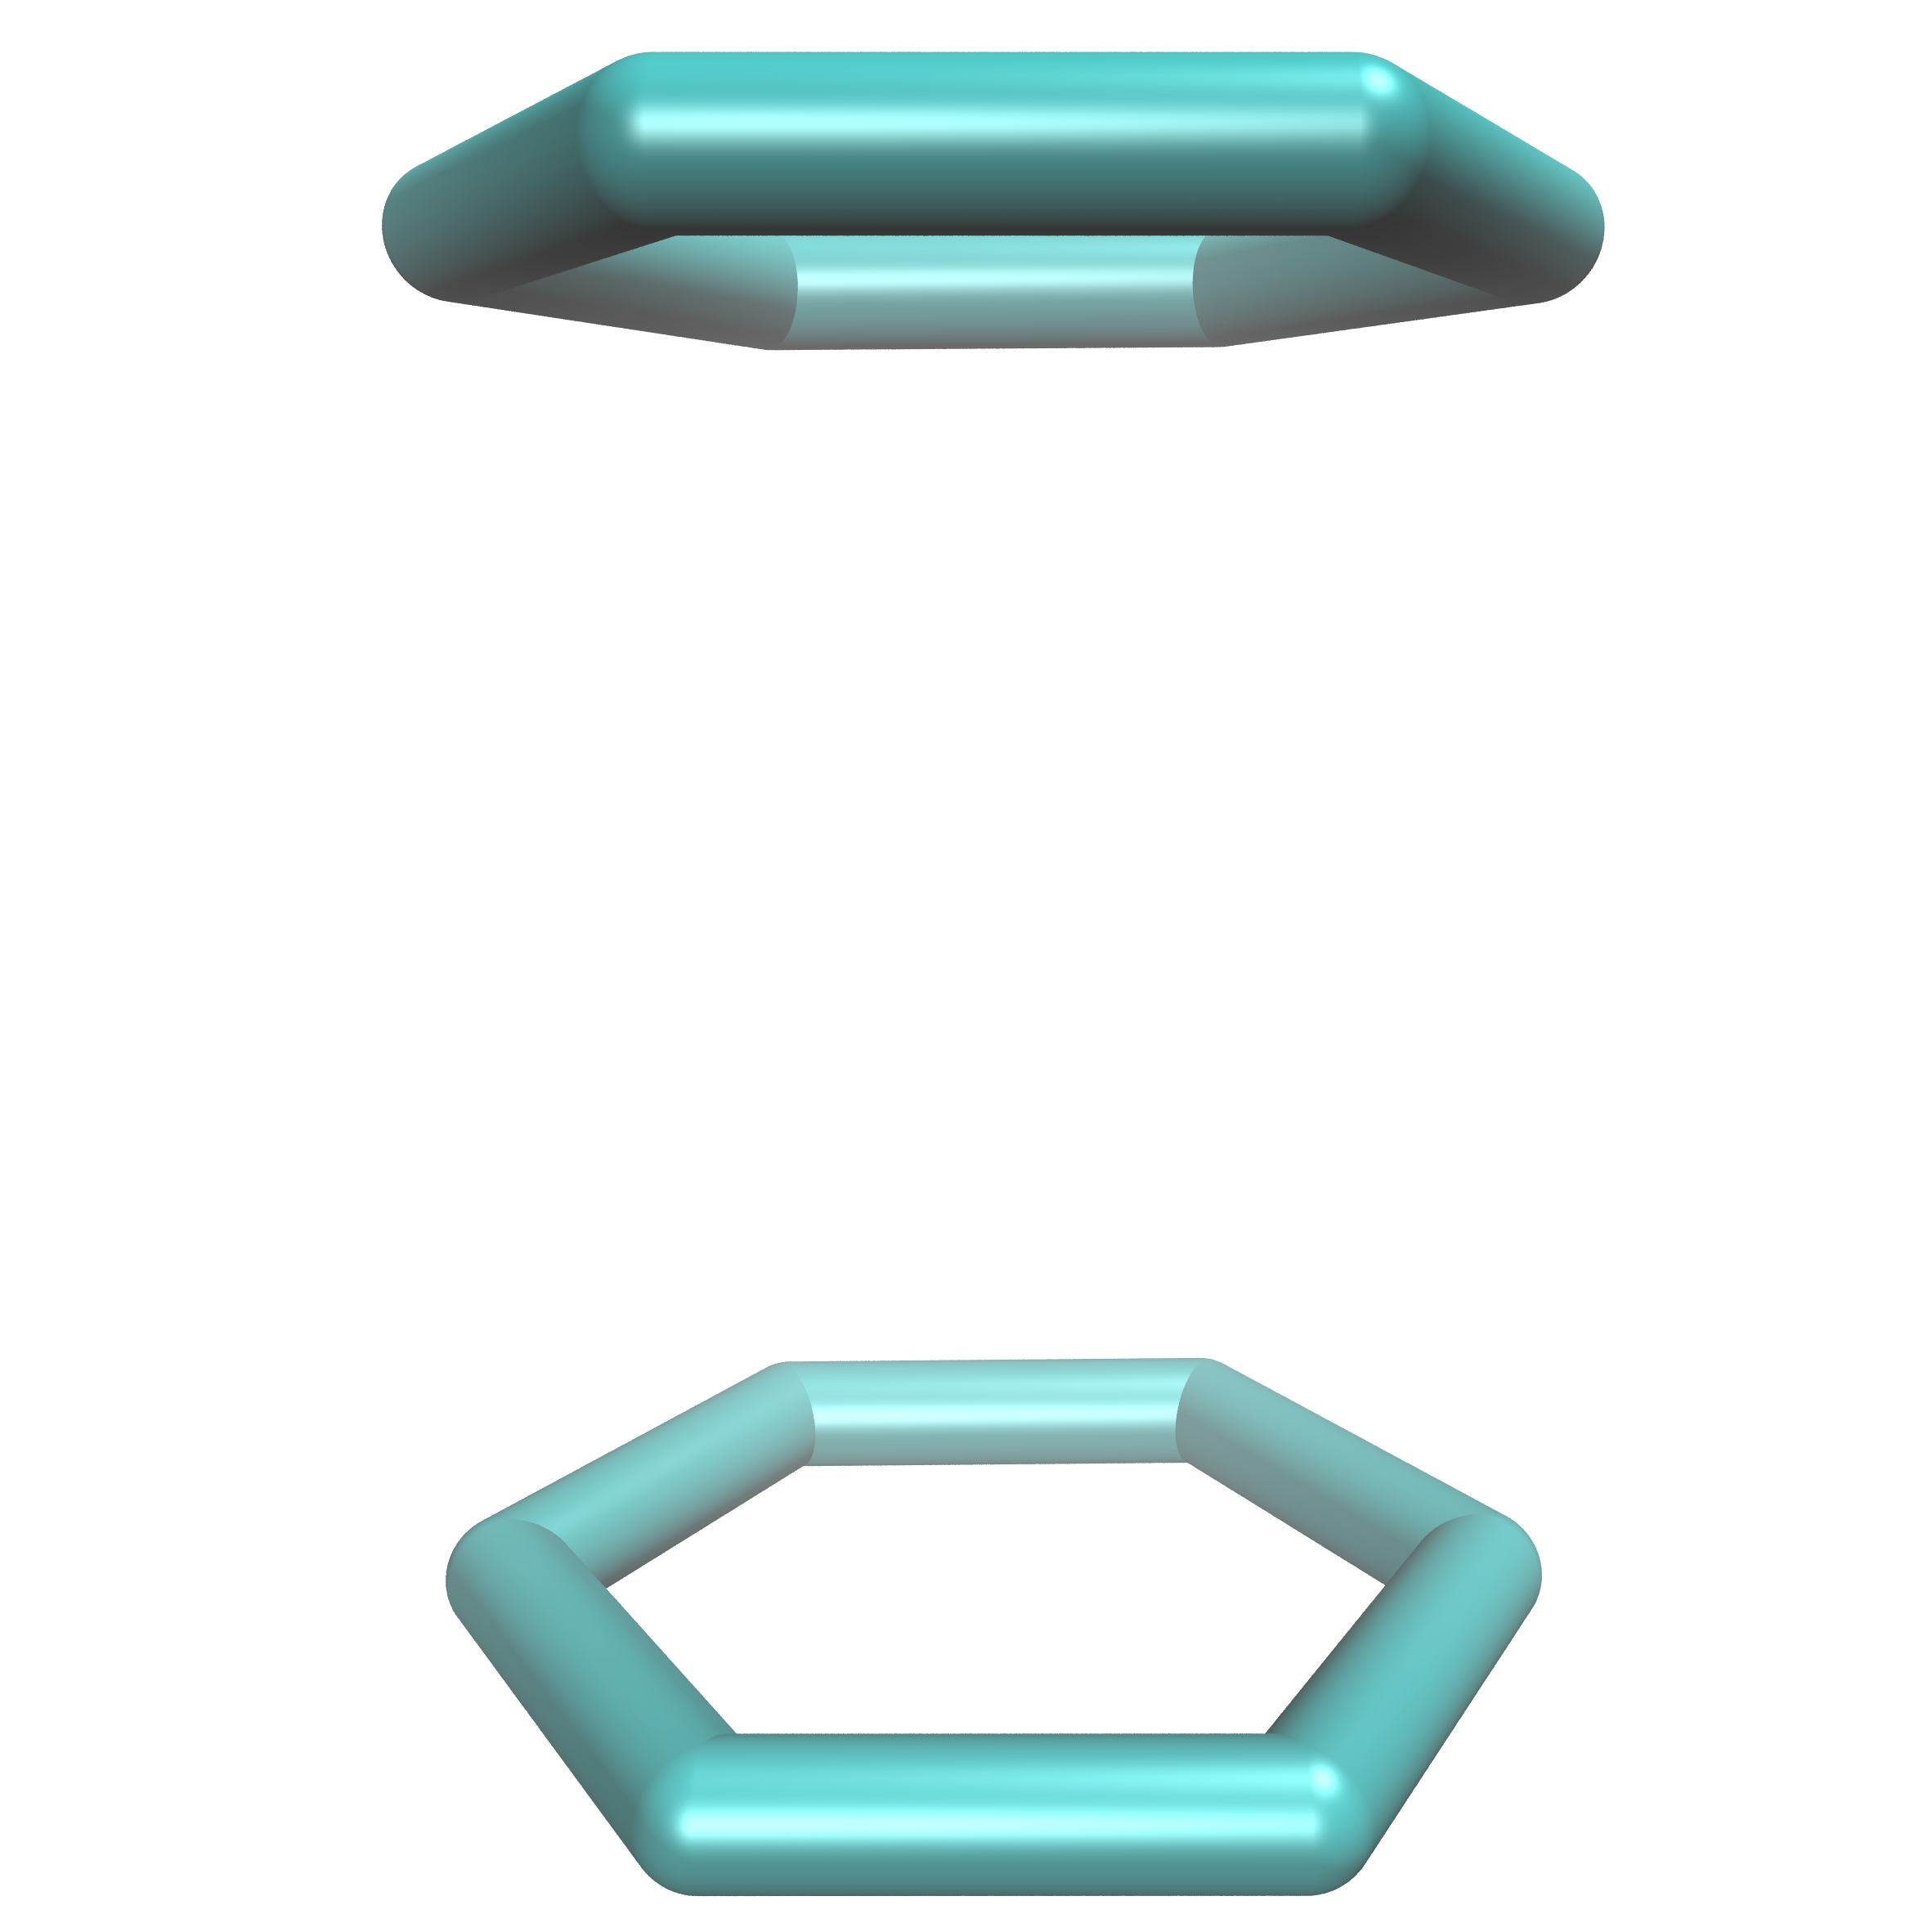
\includegraphics[width=\textwidth]{sandwiched.png}
		\caption{}\label{fig:sandwiched}
	\end{subfigure}
	\begin{subfigure}[b]{0.32\textwidth}
		\centering
		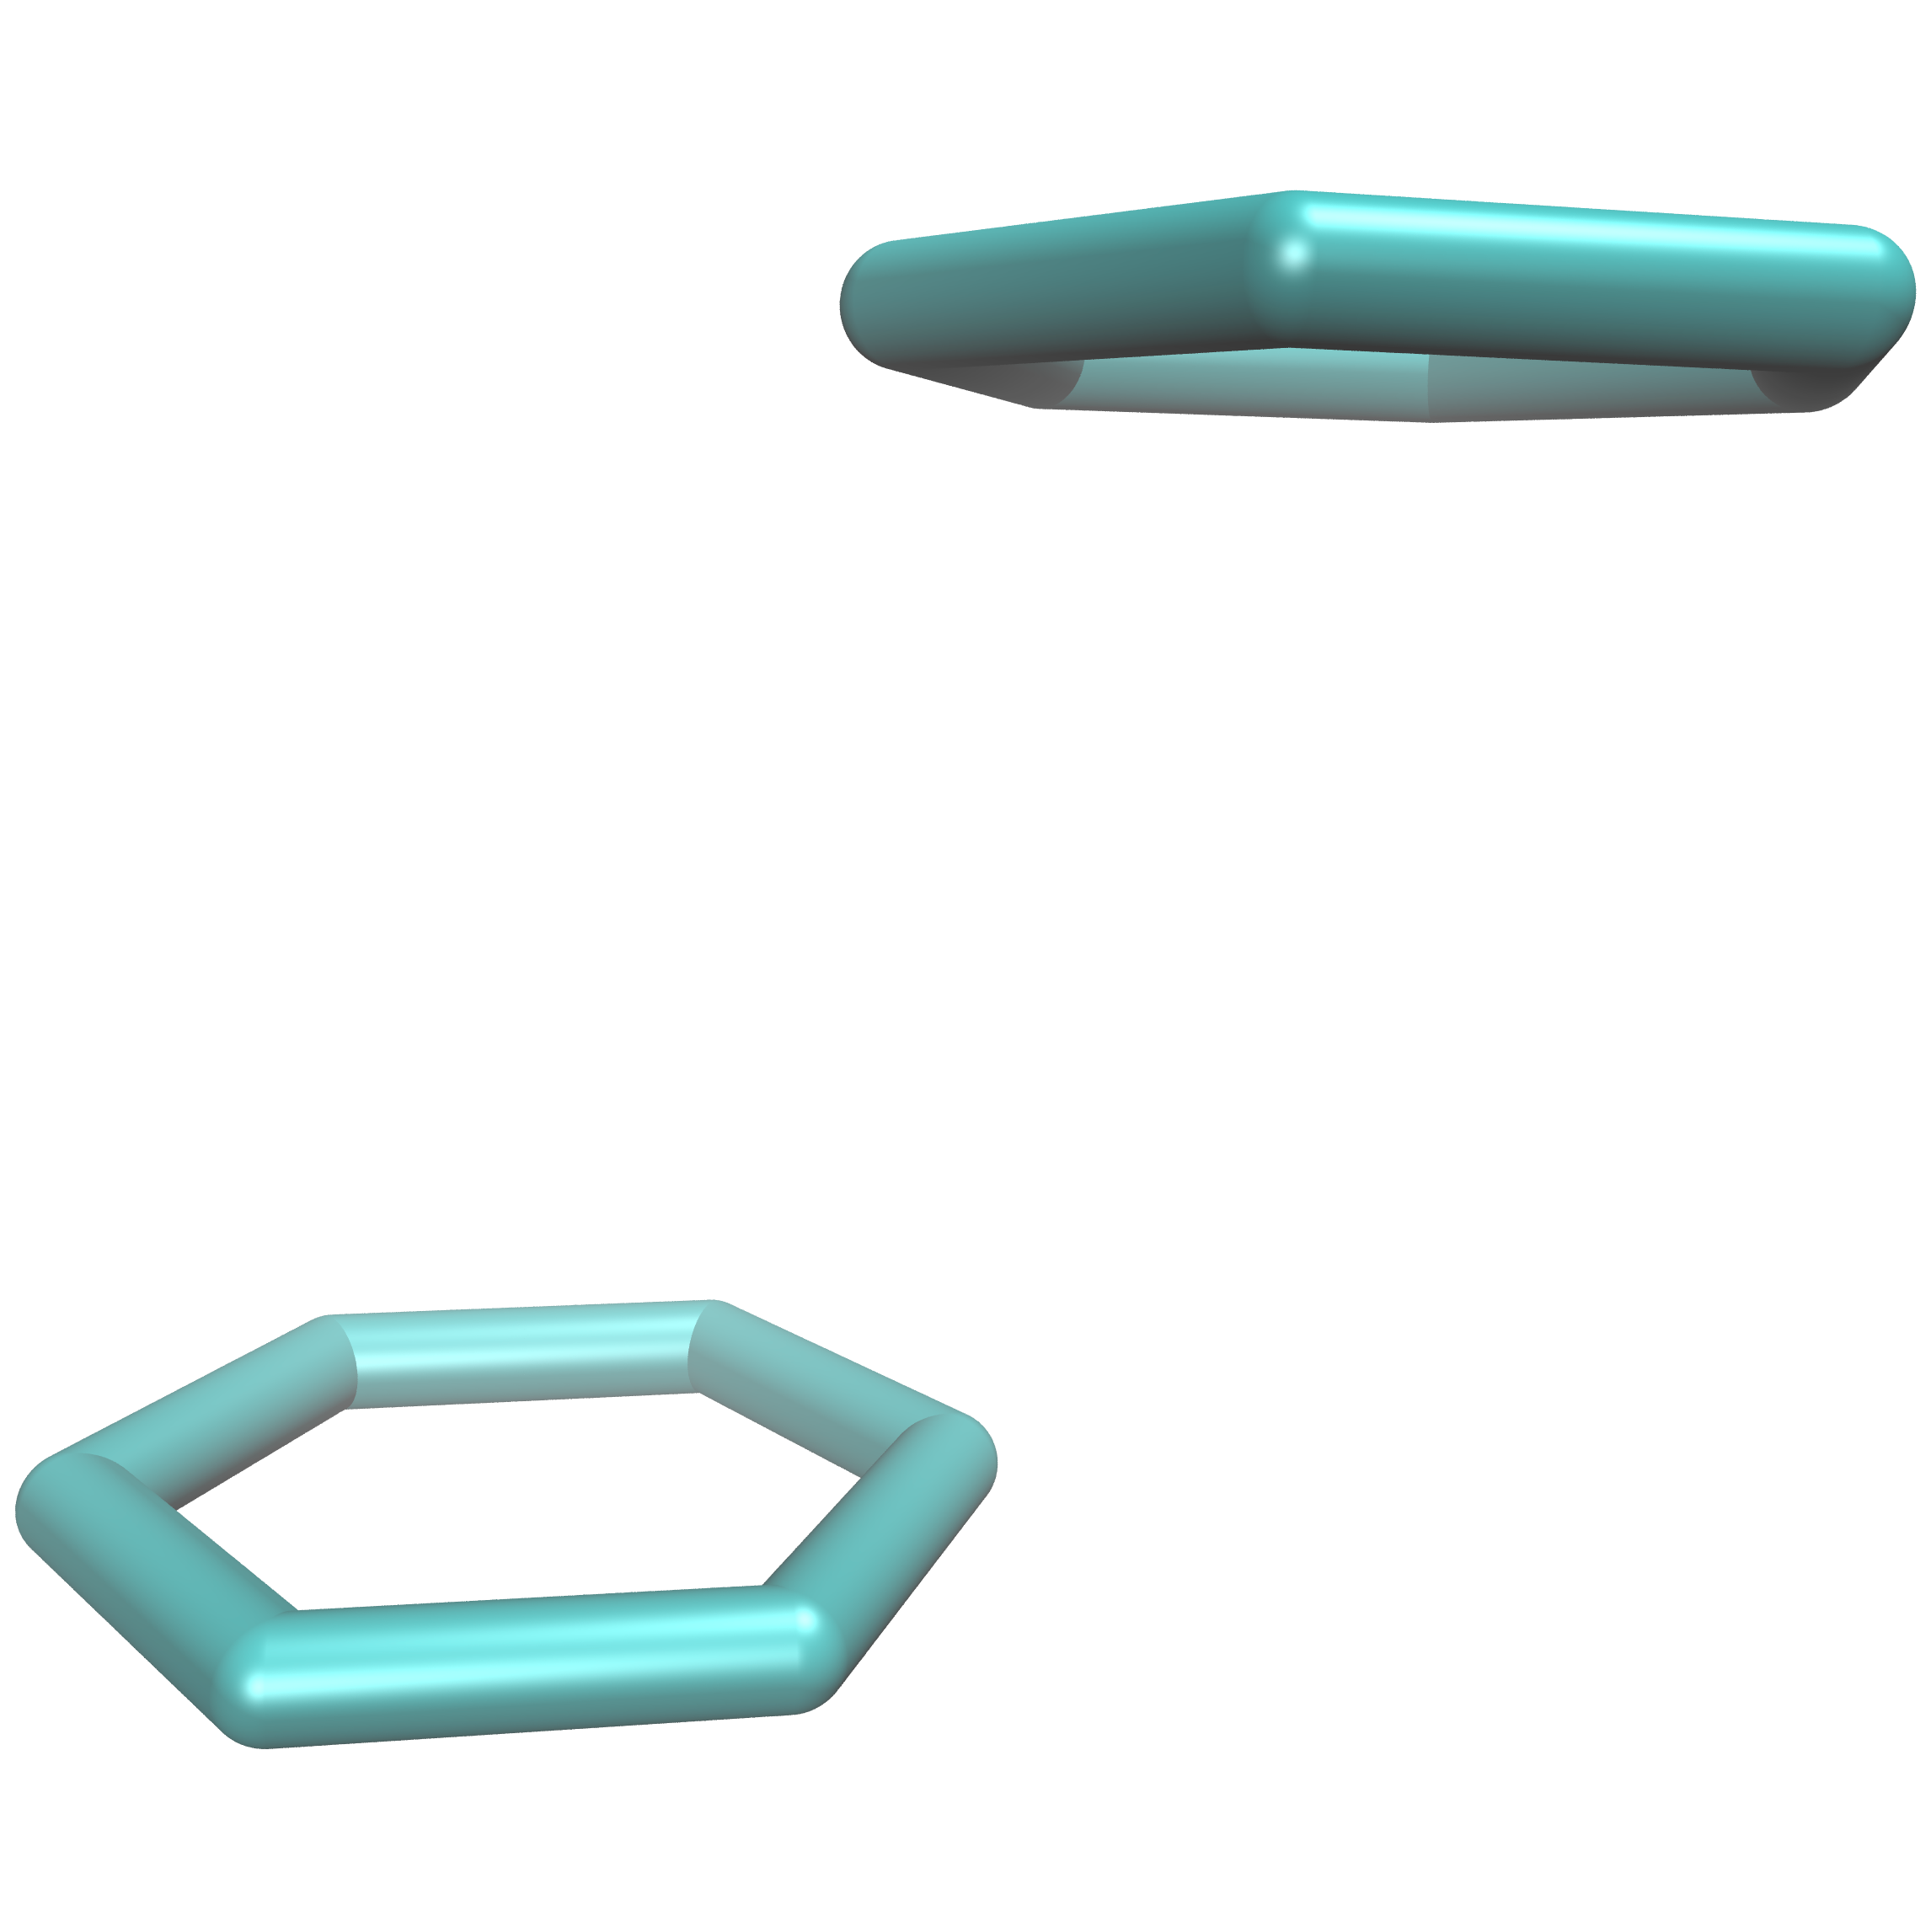
\includegraphics[width=\textwidth]{PD.png}
		\caption{}\label{fig:pd}
	\end{subfigure}
	\begin{subfigure}[b]{0.32\textwidth}
		\centering
		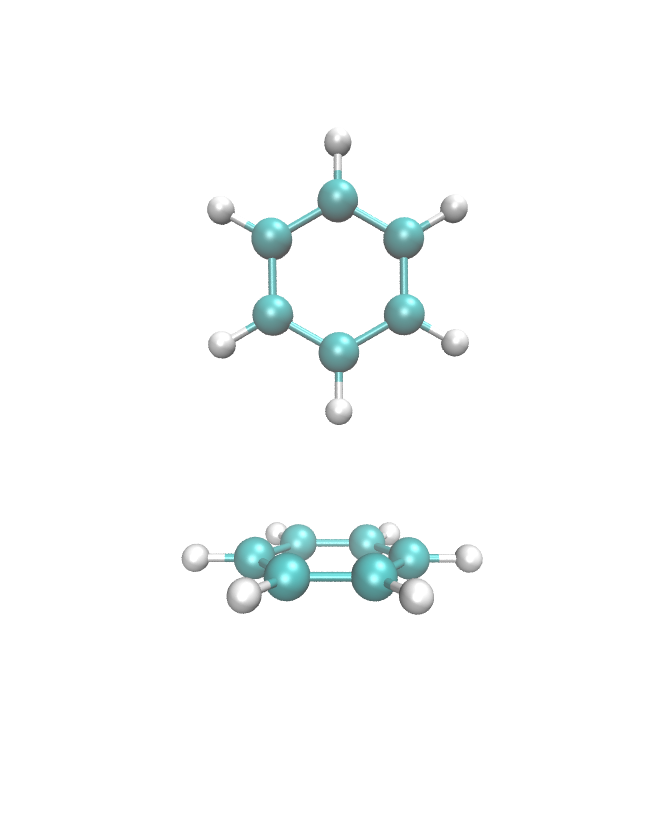
\includegraphics[width=\textwidth]{Tshaped.png}
		\caption{}\label{fig:tshaped}
	\end{subfigure}
	\vskip\baselineskip
	\begin{subfigure}[b]{0.475\textwidth}
		\centering
		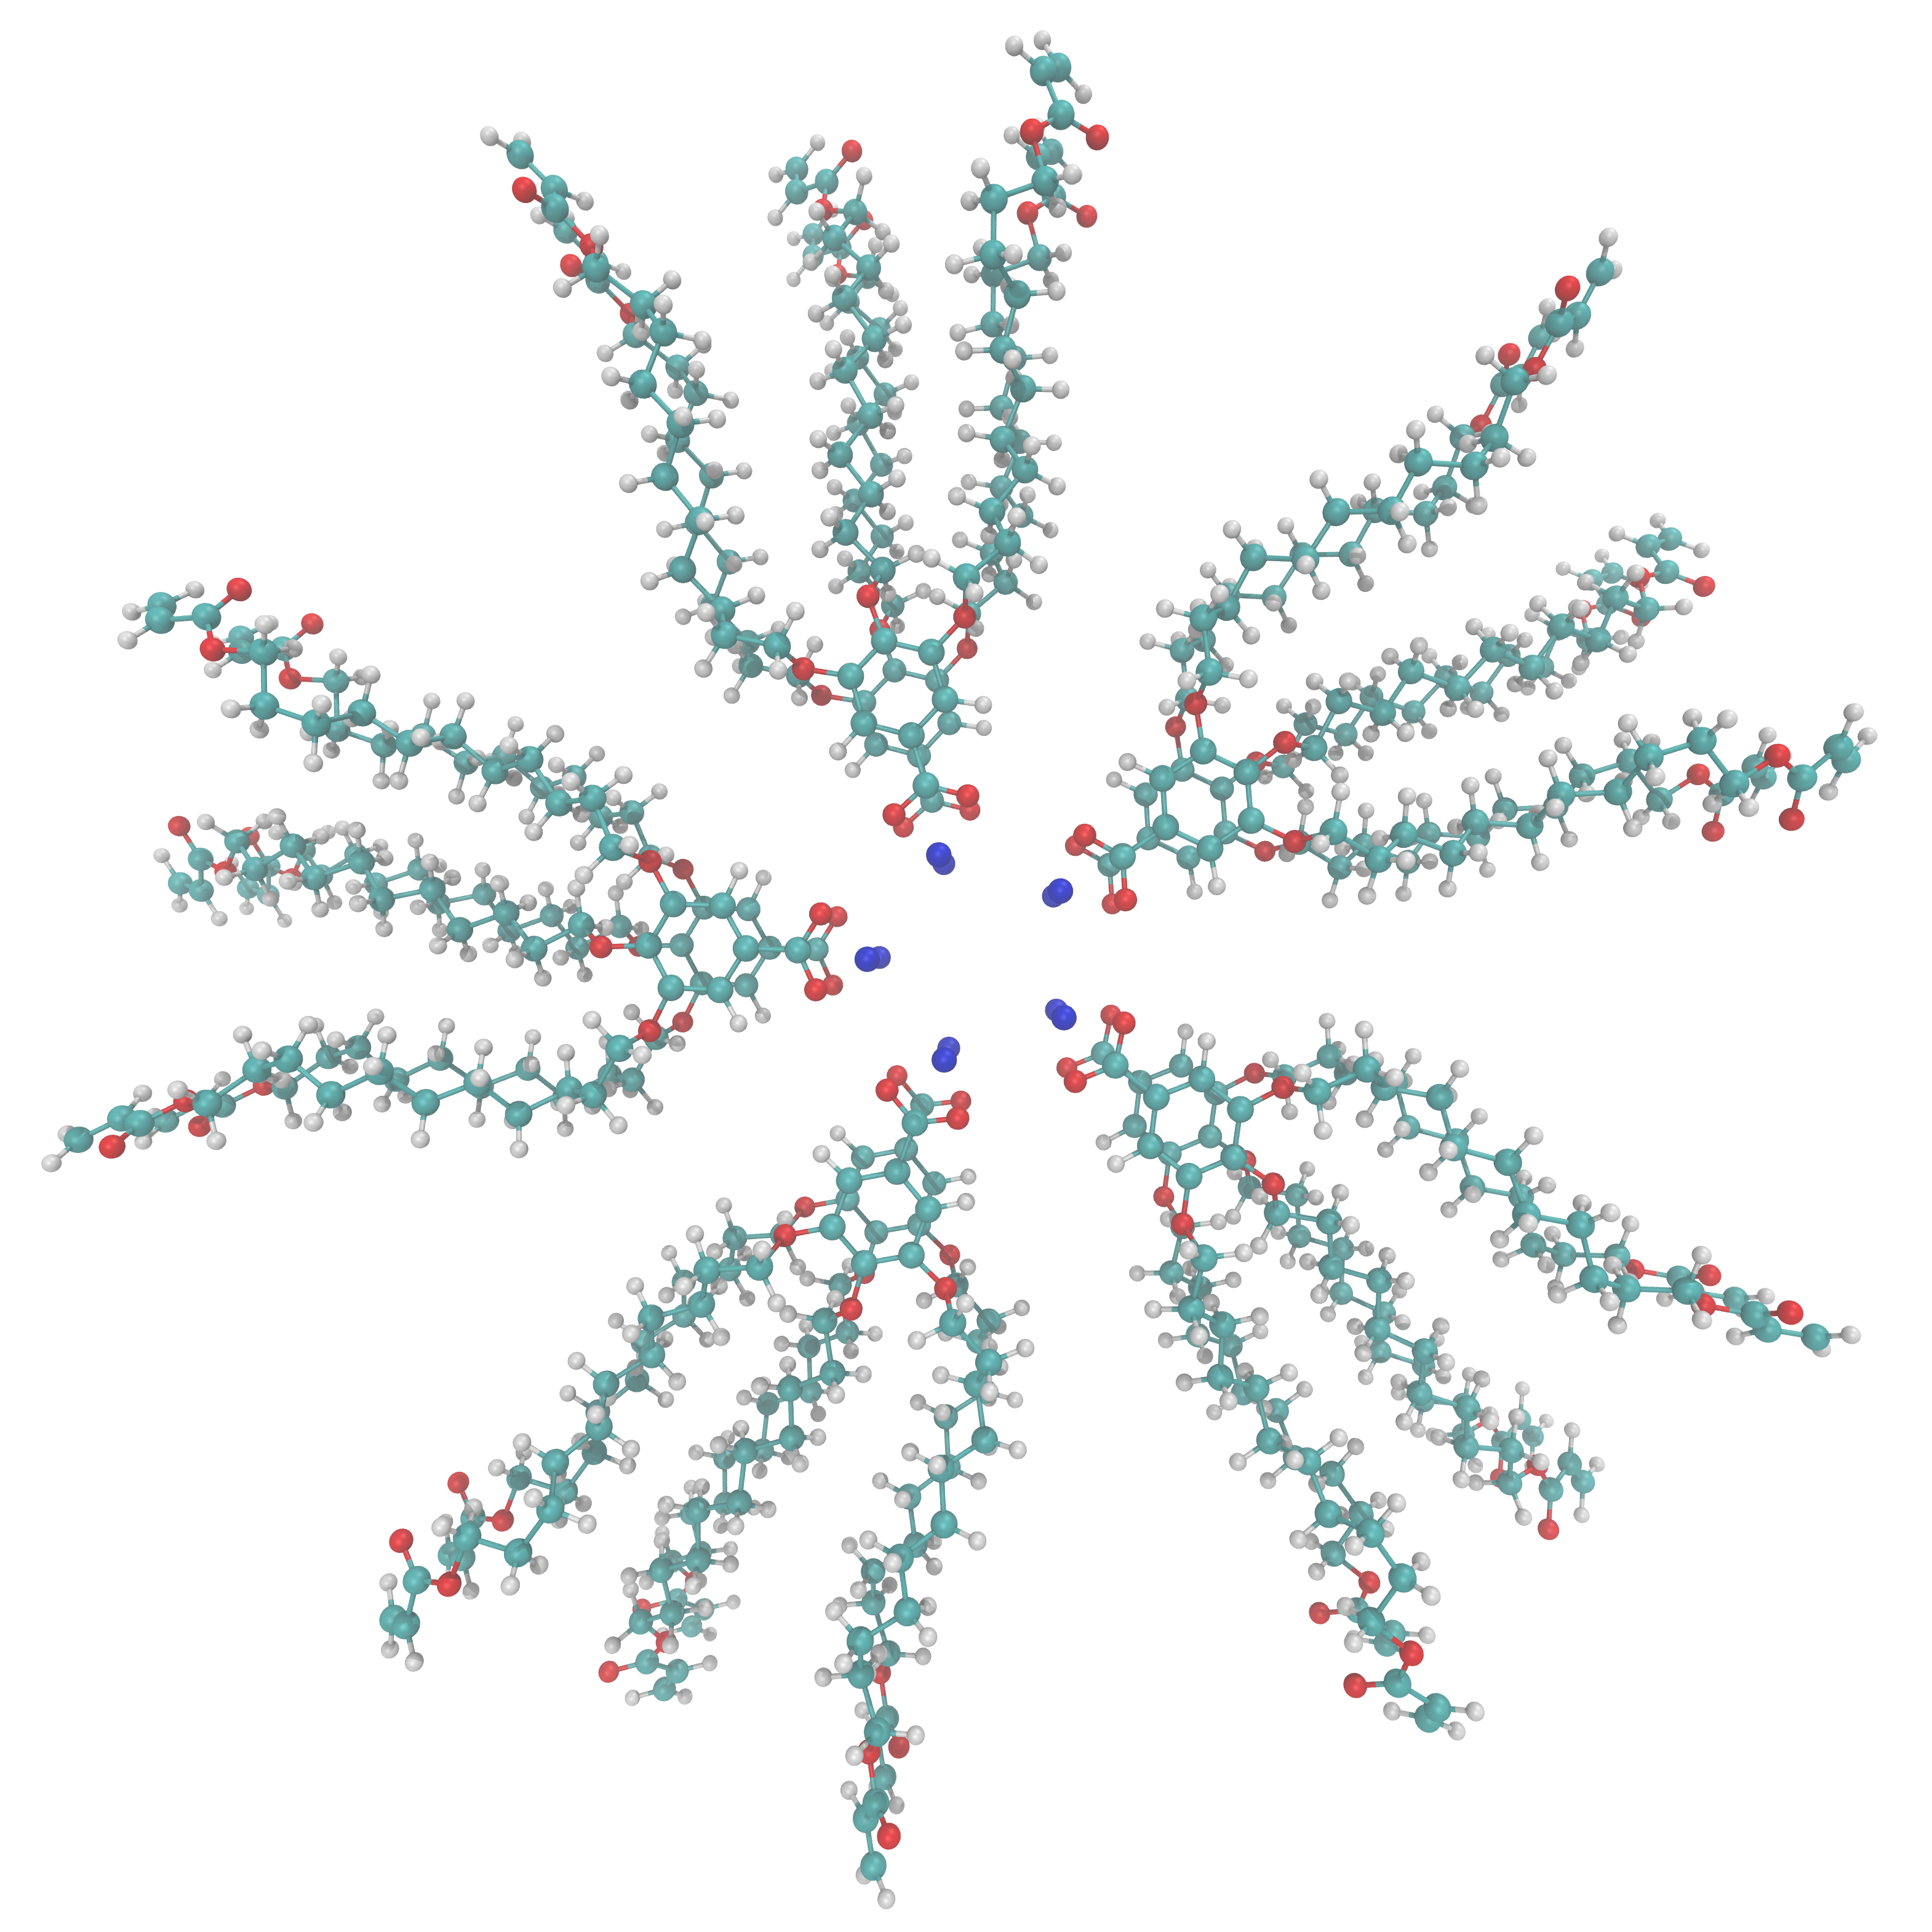
\includegraphics[width=\textwidth]{sandwichedlayers.png}
		\caption{}\label{fig:sandwichedlayers}
	\end{subfigure}
	\begin{subfigure}[b]{0.475\textwidth}
		\centering
		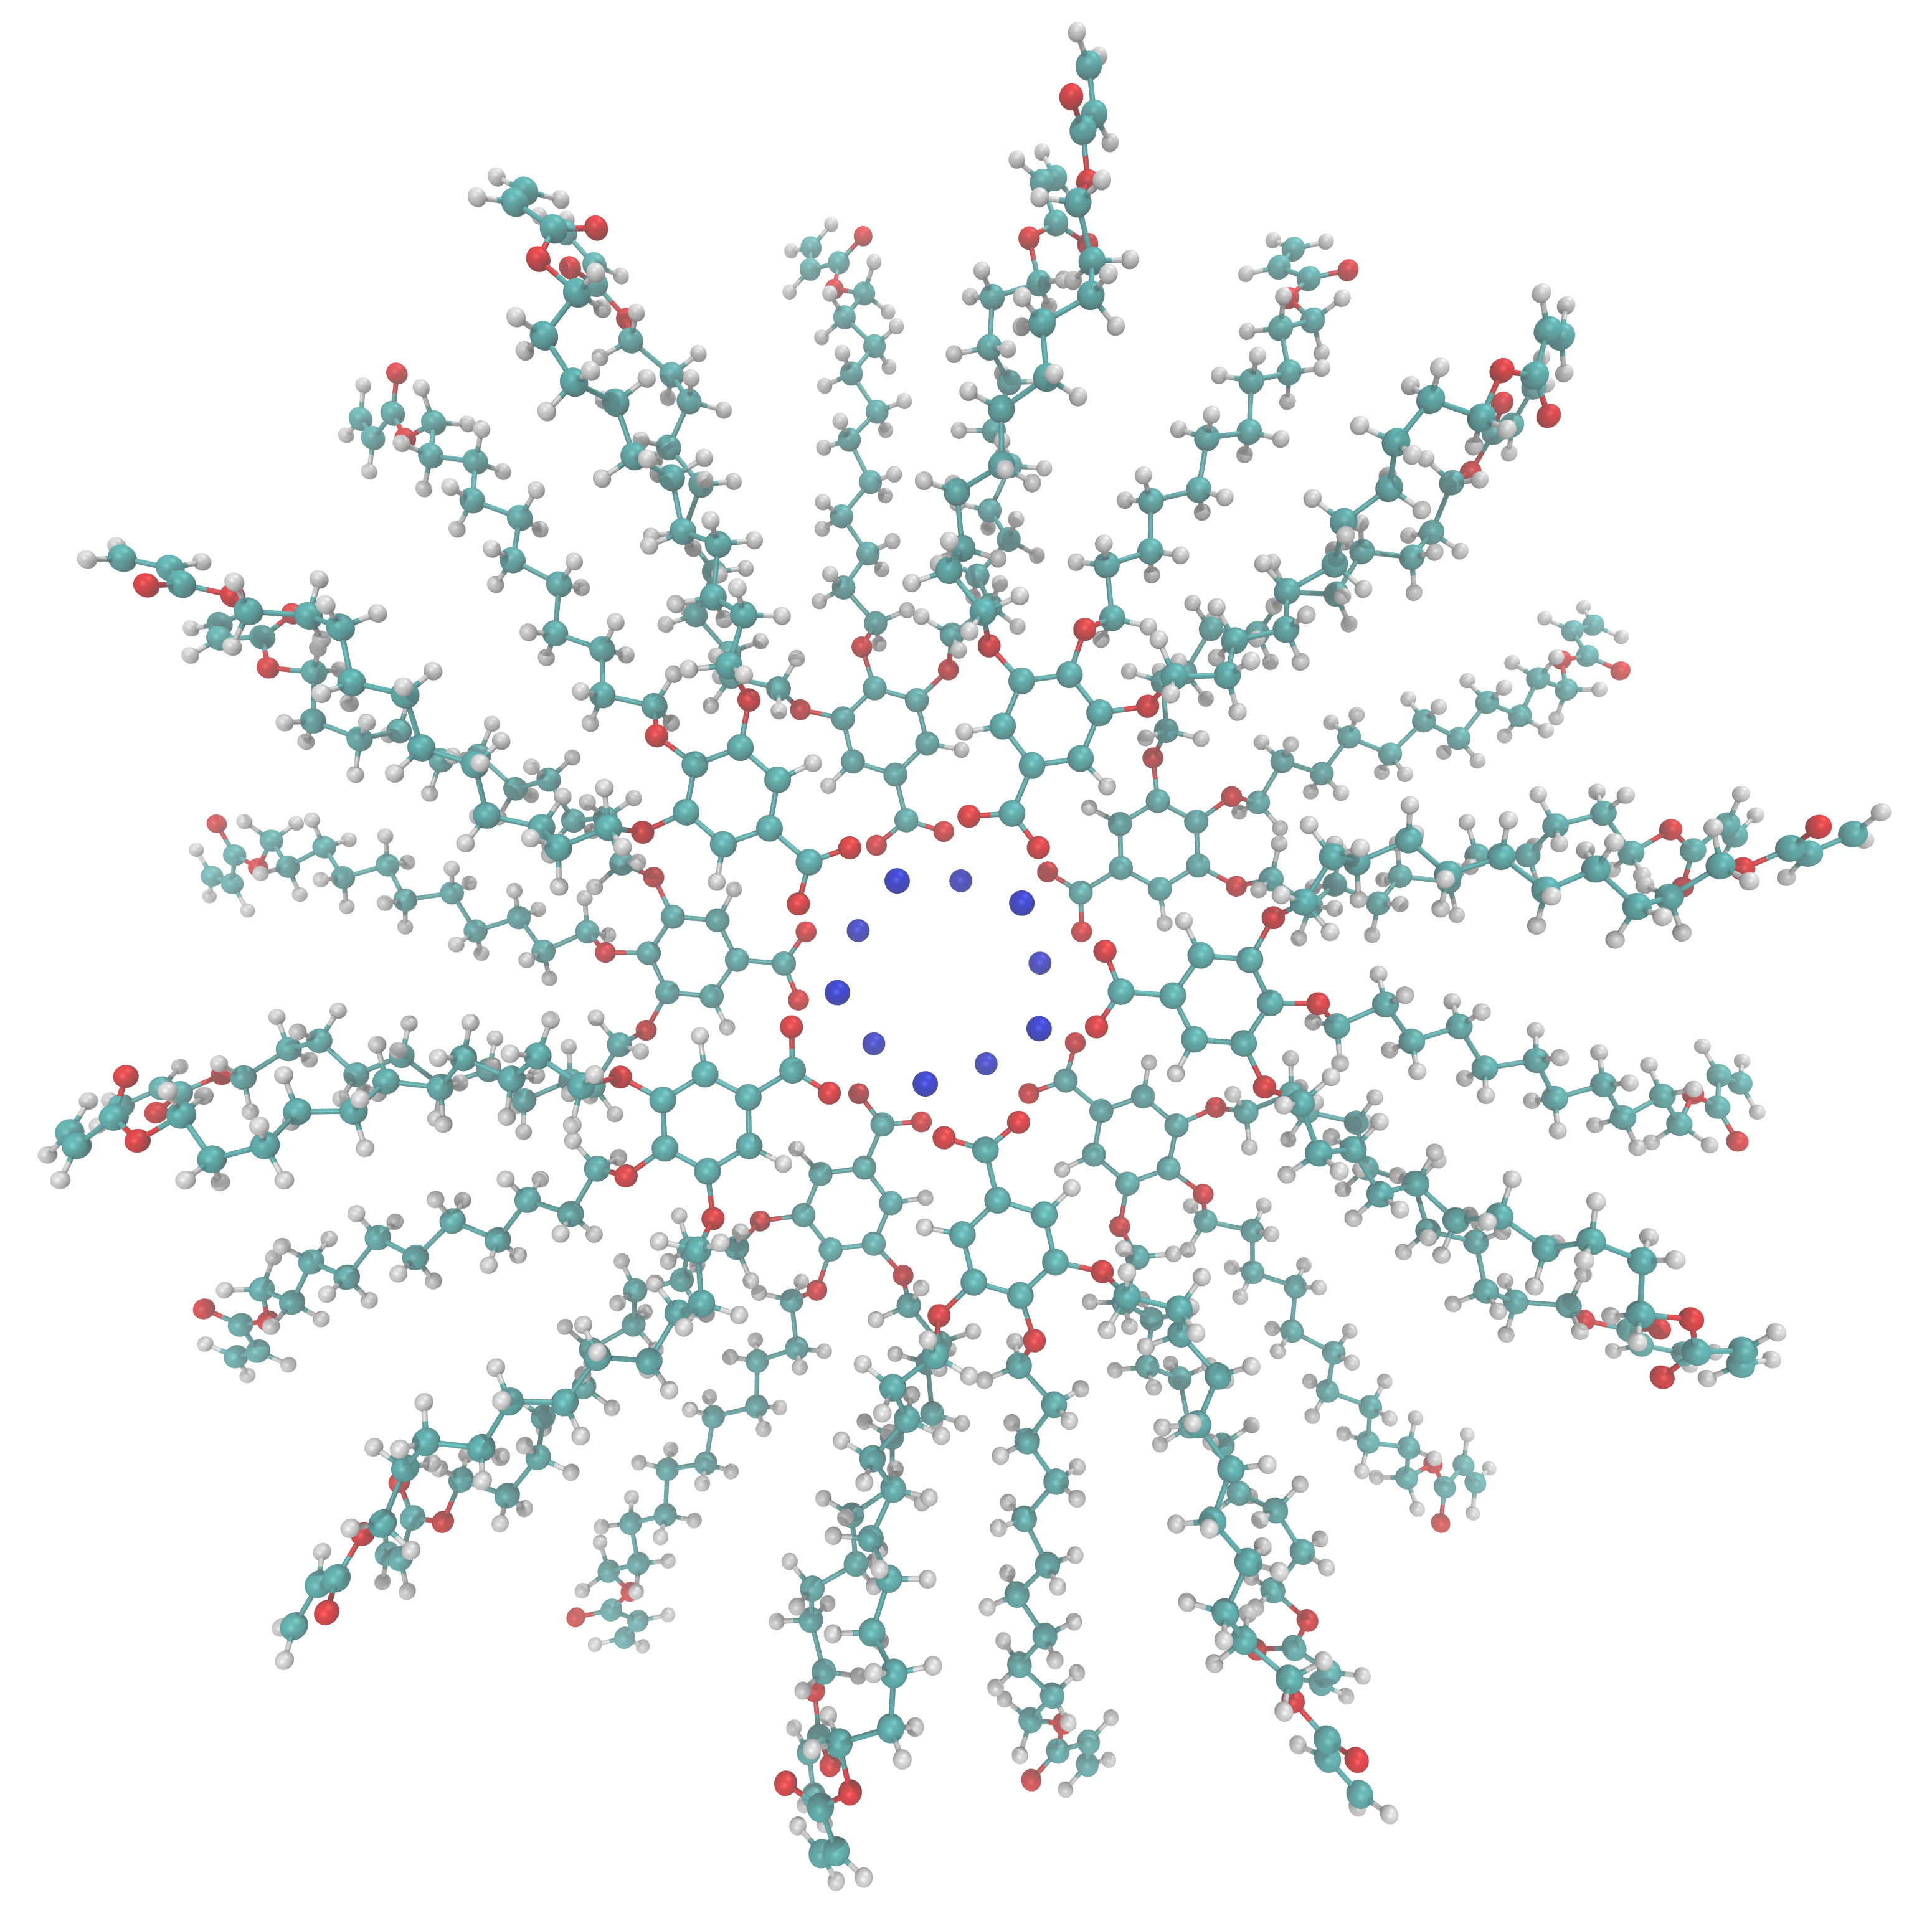
\includegraphics[width=\textwidth]{offsetlayers.png}
		\caption{}\label{fig:offsetlayers}
	\end{subfigure}
	\caption{(a) Sandwiched benzene dimers stack 3.8 \angstrom~apart. (b) Parallel-Displaced benzene dimers stack
	3.4 \angstrom~vertically and 1.6 \angstrom~horizontally apart. (c) T-shaped benzene dimers stack 5.0 \angstrom~apart. 
	(d) Two monomer layers stacked in the sandwiched configuration (e) Two monomer layers stacked in the parallel-displaced
	configuration }\label{fig:stacking}
  \end{figure}
  
  We explored the pore composition by measuring the average number densities of
  various monomer components as a function of distance from the pore centers.  We
  looked at the average number density of sodium ions, aromatic rings and carbon
  atoms making up the monomer tails. The radial distance of all atoms in each
  group from the pore centers are binned, then normalized by the volume of the
  annulus defined by the bin edges and z box vector.
  %BJC: Maybe write an equation here? It's hard to say precisely how I did it
  %in words without it sounding confusing 

  We calculated ionic conductivity using two different methods for robustness.
  The Nernst-Einstein relation relates the DC ionic conductivity to ion
  diffusivity, $D$, concentration, $C$, ion charge, $q$, the boltzmann constant,
  $k_b$, and temperature, $T$: $$\sigma = \dfrac{q^2CD}{k_b T}$$ 
  Sodium ion diffusion coefficients were found by calculating the slope
  of the linear region of the z-direction mean square displacement curve as
  indicated by the einstein relation \cite{einstein_investigations_1956}. We
  visualized the MSD plot to determine where to begin and end a linear fit. Ion
  concentration was measured with respect to the volume of the entire unit cell. 

  The second method, termed the Collective Diffusion model, measures the
  movement of the collective variable, Q, which is defined as the amount of
  charge transfer through the system and can be thought to represent the center
  of charge of the system. The conductance, $\gamma$ of the system can be
  calculated as: $$ \gamma = \dfrac{D_Q}{k_b T} $$ Conversion to ionic
  conductivity is achieved by multiplying by channel length and dividing by the
  membrane cross sectional area.  $D_Q$ is the diffusion coefficient of the
  collective variable Q. It can be calculated using the einstein relation.  A
  full derivation of the model can be accessed elsewhere 
  \cite{liu_collective_2013}.

  \section{Results and Discussion}
  
%  \subsection{Determination of Nanoscopic Structural Details}
  \subsection{Determining the Spatial Configuration of Monomers}

  Our simulations best support a model built with 5 monomers per layer based on
  the measured equilibrated pore-to-pore distances. To discern the composition of
  the monomer layers, addressing (\ref{point:monomernum}), we ran simulations of
  systems created with 4 - 8 monomers per layer. Systems were built in both the
  parallel displaced and sandwiched configurations with layers initially spaced
  3.7 \AA~apart. Equilibrated configurations were prepared according to the dry
  equilibration procedure. All systems are stable after 400 ns of simulation. In
  a sense, all systems are at least metastable, addressing
  (\ref{point:metastable}), however not all will make physical sense or fit the
  experimental profile that we are looking to match. Figure~\ref{fig:p2p} shows
  the pore spacing for all systems tested. Systems built with 5 monomers in each
  layer equilibrate to a pore spacing that is most consistent with the
  experimental value of 4.12 nm derived from SAXS measurements
  (Figure~\ref{fig:SAXS}). The remainder of this discussion will focus on the
  analysis of systems built with 5 monomers per layer.

  \begin{figure}
	\centering
	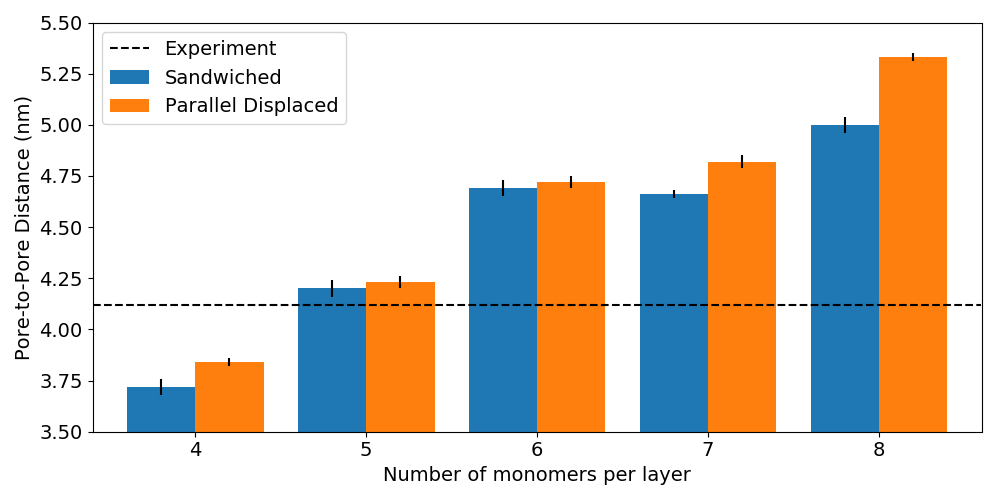
\includegraphics[width=\linewidth]{p2p.png}
	\caption{Systems built with 5 monomers per layer in a parallel
		displaced configuration result in a pore spacing closest to the experimental
		value of 4.12 nm. The pore spacing of the model increases as number of monomers
		in each layer increases. The pore spacing of a system starting in the
		sandwiched configuration is systematically lower than that started in an offset
		configuration. }~\label{fig:p2p}
  \end{figure}  

  We learned that layers are well-defined and persistent, answering
  (\ref{point:layers}). We established our conclusion by plotting the pair
  correlation function, $g(z)$, calculated between atoms along the length of the
  pores (Fig.~\ref{fig:zdf}). We measured $g(z)$ with respect to aromatic rings in
  the head groups and, separately, with respect to carbon atoms in the alkane
  chains. Using a fourier transform of $g(z)$, we see that sandwiched
  configuration layers stack 4.39 \angstrom~ apart while parallel displaced
  configuration layers stack 4.38 \angstrom~ apart.

  %BJC: TODO: increase font size on legends
  \begin{figure}
        \centering
        \begin{subfigure}{0.45\textwidth}
                \centering
                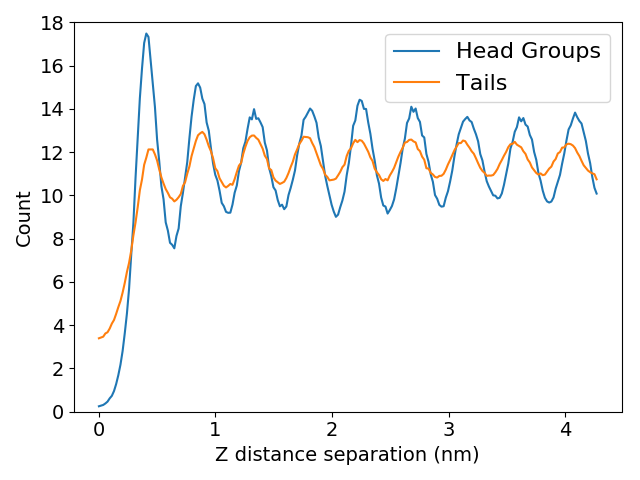
\includegraphics[width=\textwidth]{zdf_overlay_layered.png}
                \caption{}\label{fig:zdf_layered}
        \end{subfigure}
        \begin{subfigure}{0.45\textwidth}
                \centering
                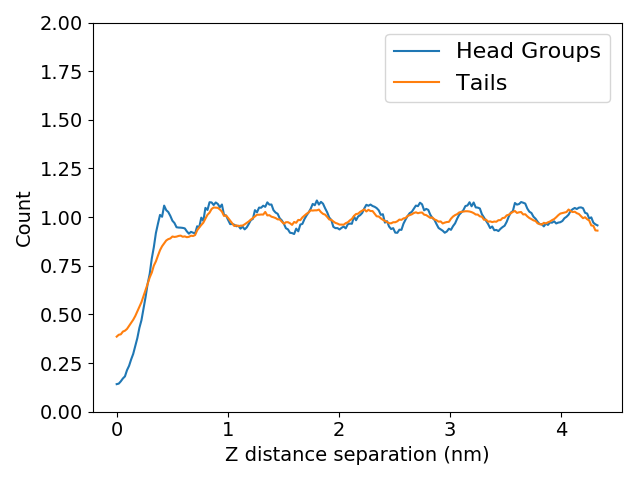
\includegraphics[width=\textwidth]{zdf_overlay_offset.png}
                \caption{}\label{fig:zdf_offset}
        \end{subfigure}
        \caption{Pair distribution functions of aromatic carbons for the
        (a) 5 monomer per layer, sandwiched and (b) 5 monomer per layer,
        parallel displaced configurations. Clear periodic maxima in the
        $z$ number density indicate distinct layers. The magnitude
        of the spikes with respect to the average suggest that the 5
        monomer per layer, sandwiched configuration possesses a higher
        degree of layer partitioning.}\label{fig:zdf}
  \end{figure}

  We answer question (\ref{point:orientation}) by simulating X-ray diffraction
  patterns produced from equilibrated MD trajectories. We tested systems built
  with 5 monomers per layer in the parallel displaced and sandwiched
  configurations. Simulated patterns were generated using portions of simulation
  trajectory after equilibration. The patterns for both structures are shown and
  compared to experiment in Figure \ref{fig:XRDsim}.

  Simulated XRD of the sandwiched configuration contains all experimental
  features except for R-helix. R-alkanes, R-spots and R-pores appear close to their
  expected locations. R-$\pi$ is also present, however it intersects R-alkanes at
  a $q_z$ value lower than experiment meaning the head groups in our model prefer 
  to stack farther apart. 

  The parallel displaced configuration results in a simulated XRD pattern with
  the closest match to experiment. It produces the only pattern that exhibits all
  major reflections. R-alkanes and R-pores appear as they do in the
  sandwiched configuration. R-spots and R-$\pi$ appears, however with a lower intensity relative to
  R-alkanes when compared to the sandwiched configuration. R-helix appears due to
  the parallel displaced aromatic rings. It is a subharmonic of R-$\pi$ since the
  nearest vertically stacked head group to any given head group is 7.4 \AA~ away. 

  %BJC: adjust figure size and alignment -- probably easiest to set figure size in matplotlib
  \begin{figure}
  \begin{subfigure}{0.3\linewidth}
        \centering
        \vspace{-0.2em}
        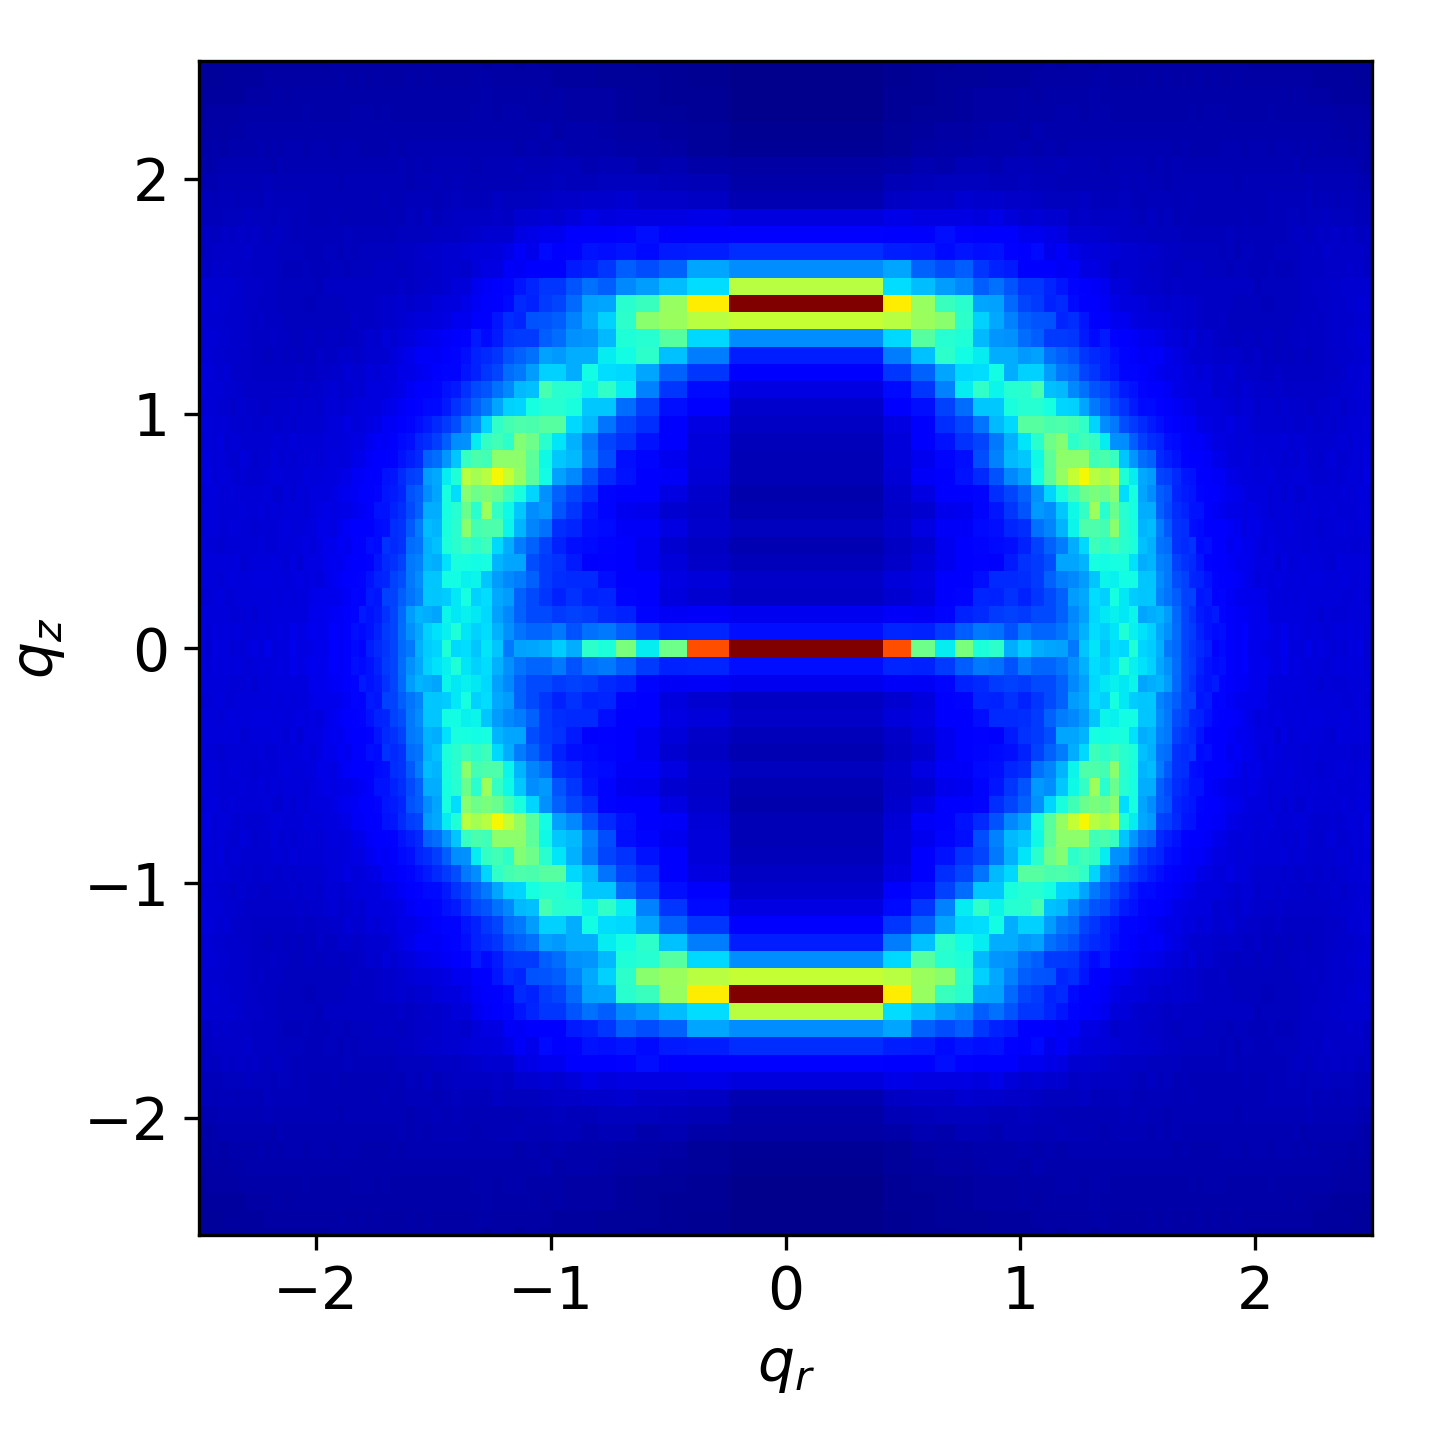
\includegraphics[width=1.018\linewidth]{layered_rzplot.png}
        \caption{}~\label{fig:rz_layered}
  \end{subfigure}
  \begin{subfigure}{0.3\linewidth}
        \centering
%        \vspace{0.25em}
        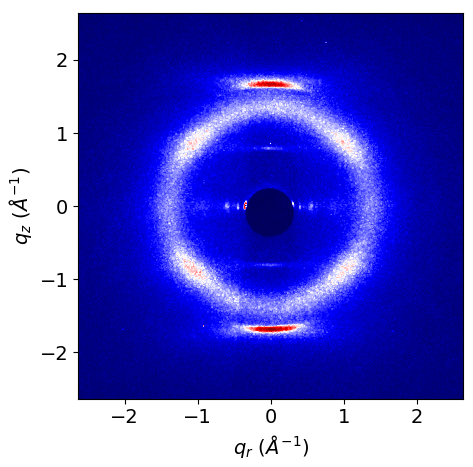
\includegraphics[scale=0.29]{WAXS_raw.png}
        \caption{}~\label{fig:raw_waxs}
  \end{subfigure}
  \begin{subfigure}{0.3\linewidth}
        \centering
        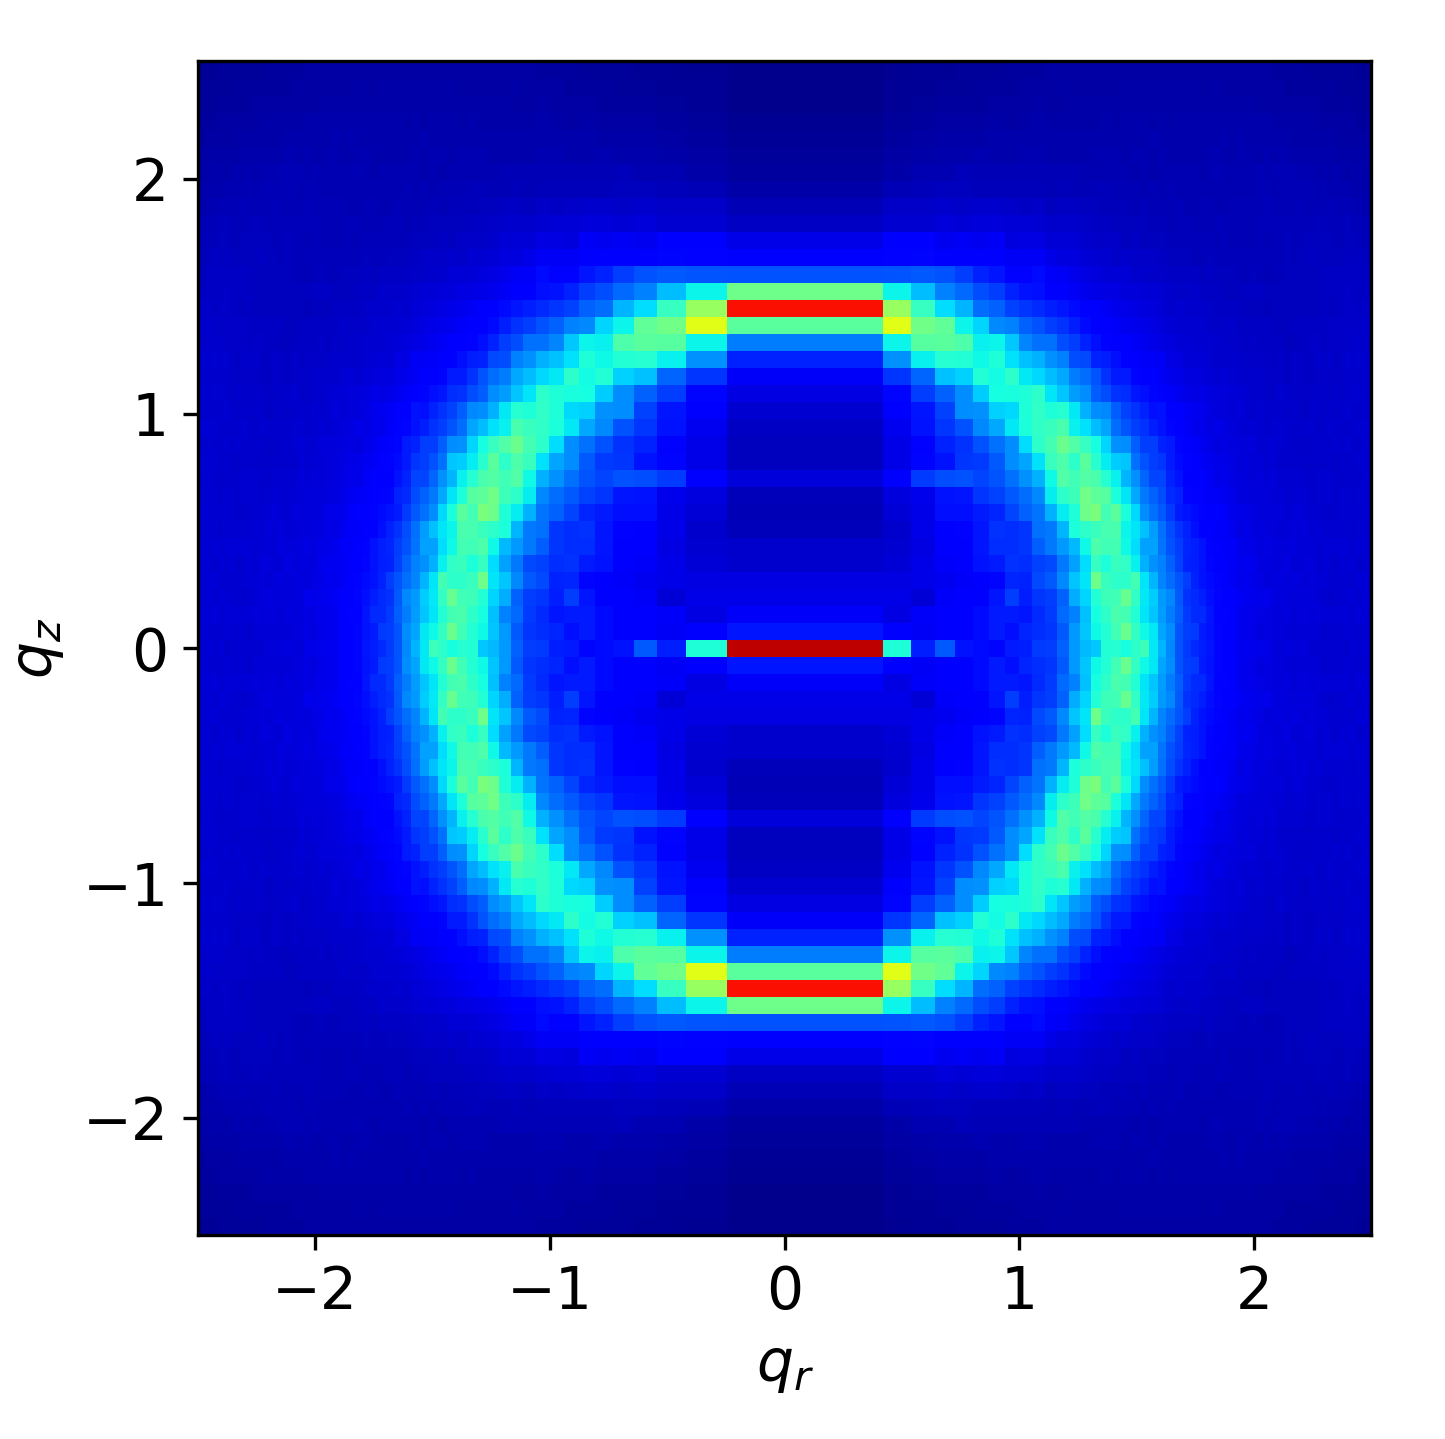
\includegraphics[width=\linewidth]{offset_rzplot.png}
        \caption{}~\label{fig:rz_offset}
  \end{subfigure}
  \begin{subfigure}{0.0544\linewidth}
        \centering
        \vspace{-3.30em}
        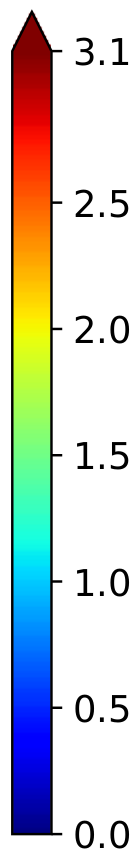
\includegraphics[width=\linewidth]{colorbar_jet.png}
  \end{subfigure}
  \caption{The simulated X-ray diffraction patterns for simulations run in the
  sandwiched (a) and parallel-displaced (c) configurations are compared to experiment (b). 
  The parallel displaced configuration is the only one that exhibits all major
  reflections of interest to some degree}
  \label{fig:XRDsim}
  \end{figure}

%  In both simulated diffraction patterns R-alkanes appears in the expected location. 
%  The location of R-pores is not well-defined in comparison to experiment. In order
%  to resolve those reflections it would be necessary to simulate a much larger system, 
%  but that is unnecessary since we can measure pore spacing manually as described 
%  earlier. R-$\pi$ and R

  In both the parallel displaced and sandwiched configurations, we noted that
  R-$\pi$ appears in a location which corresponds to a real space separation
  larger than experiment. We attribute this discrepancy to GAFF's inability to
  appropriately model the aromatic interactions which would be necessary to
  achieve the correct $\pi$-$\pi$ stacking distance. Systems have been modeled
  that exhibit the correct stacking distance, however they are typically made of
  planar molecules spanning a large area. The system we have modeled has bulky
  tails whose entropic contributions compete with the $\pi$-$\pi$ stacking
  interaction energy.  There have been efforts to model systems that contain
  $\pi$ interactions in a classical mechanical context using polarizable
  forcefields. We could implement a polarizable force field, however it is likely
  not worth the extra computational cost. If our model proves to be inadequate
  when simulating transport, we will revisit our current choice of forcefield.  

  R-spots, which appears in both simulated XRD patterns, is a result of
  hexagonal alkane chain packing. Previously, the spots in the diffraction
  pattern had been explained as the product of tilted alkane chains. We measured
  the tilt angle of the alkane chains and showed that our system equilibrates to
  an average tilt angle close to zero degrees (Fig.~\ref{fig:tilt}). To understand the
  origin of the spots, we determined which atoms gave rise to the feature. Since
  R-spots is present as higher intensity spots within R-alkanes, it is likely
  that the spots arise as a consequence of the tails. By removing all non-tail atoms from the
  trajectory and simulating a diffraction pattern, we were able to isolate the
  cause of the spots to the tails (Figure~\ref{fig:tails}). Since the tails stay
  nearly flat, we plotted the centroids of the tails and measured the angle
  between each centroid and its nearest neighbors with respect to the plane of
  the membrane. We see distinct peaks in the distribution of these angles 
  (Figure~\ref{fig:tail_packing}).

  \begin{figure}
  \centering
  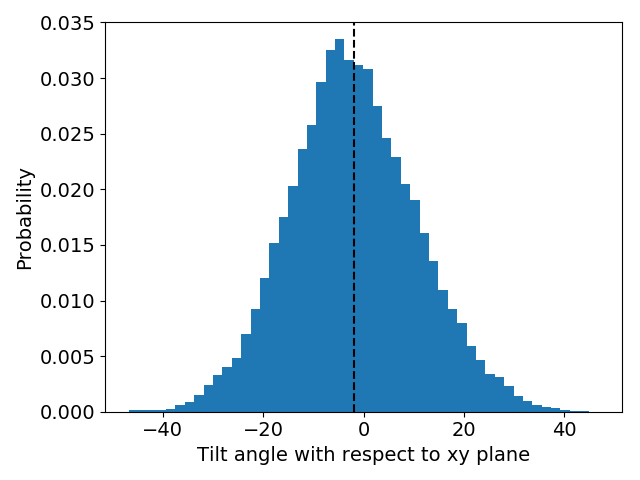
\includegraphics[width=0.5\linewidth]{tilt_dist.png}
  \caption{The tilt angle distribution of alkane chain tails with respect to the membrane plane
  indicates an average tilt angle near 7\degree~which is far from the 37\degree~tilt angle 
  previously used to explain R-spots.}~\label{fig:tilt}
  \end{figure}

  The peaks in the nearest neighbor angle distribution are consistent with the
  location of R-spots. The peaks of interest in Figures \ref{fig:offset_tails}
  and \ref{fig:layered_tails} are located at $\pm$ 33 $\degree$ which is the same
  location where the highest intensity of spots are located on the simulated
  patterns. We confirmed this conclusion by radially integrating the 2D WAXS
  pattern for $\left|\mathbf{q}\right|$ values between 1.4 and 1.57 (between 4
  and 4.5 \AA~ in real space). We observe that distinct peaks appear ca. 30
  $\degree$, in close agreement with the previously measured angle distribution
  (Figs.~\ref{fig:offset_integration}~and~\ref{fig:layered_integration}). We
  performed the same integration on the raw experimental data and found the angle
  at which R-spots reaches its highest intensity to be $\pm$ 37 $\degree$ which
  is a reconcilable difference with our simulated results.  

  \begin{figure}
	\centering
	\begin{subfigure}{0.45\linewidth}
		\centering
		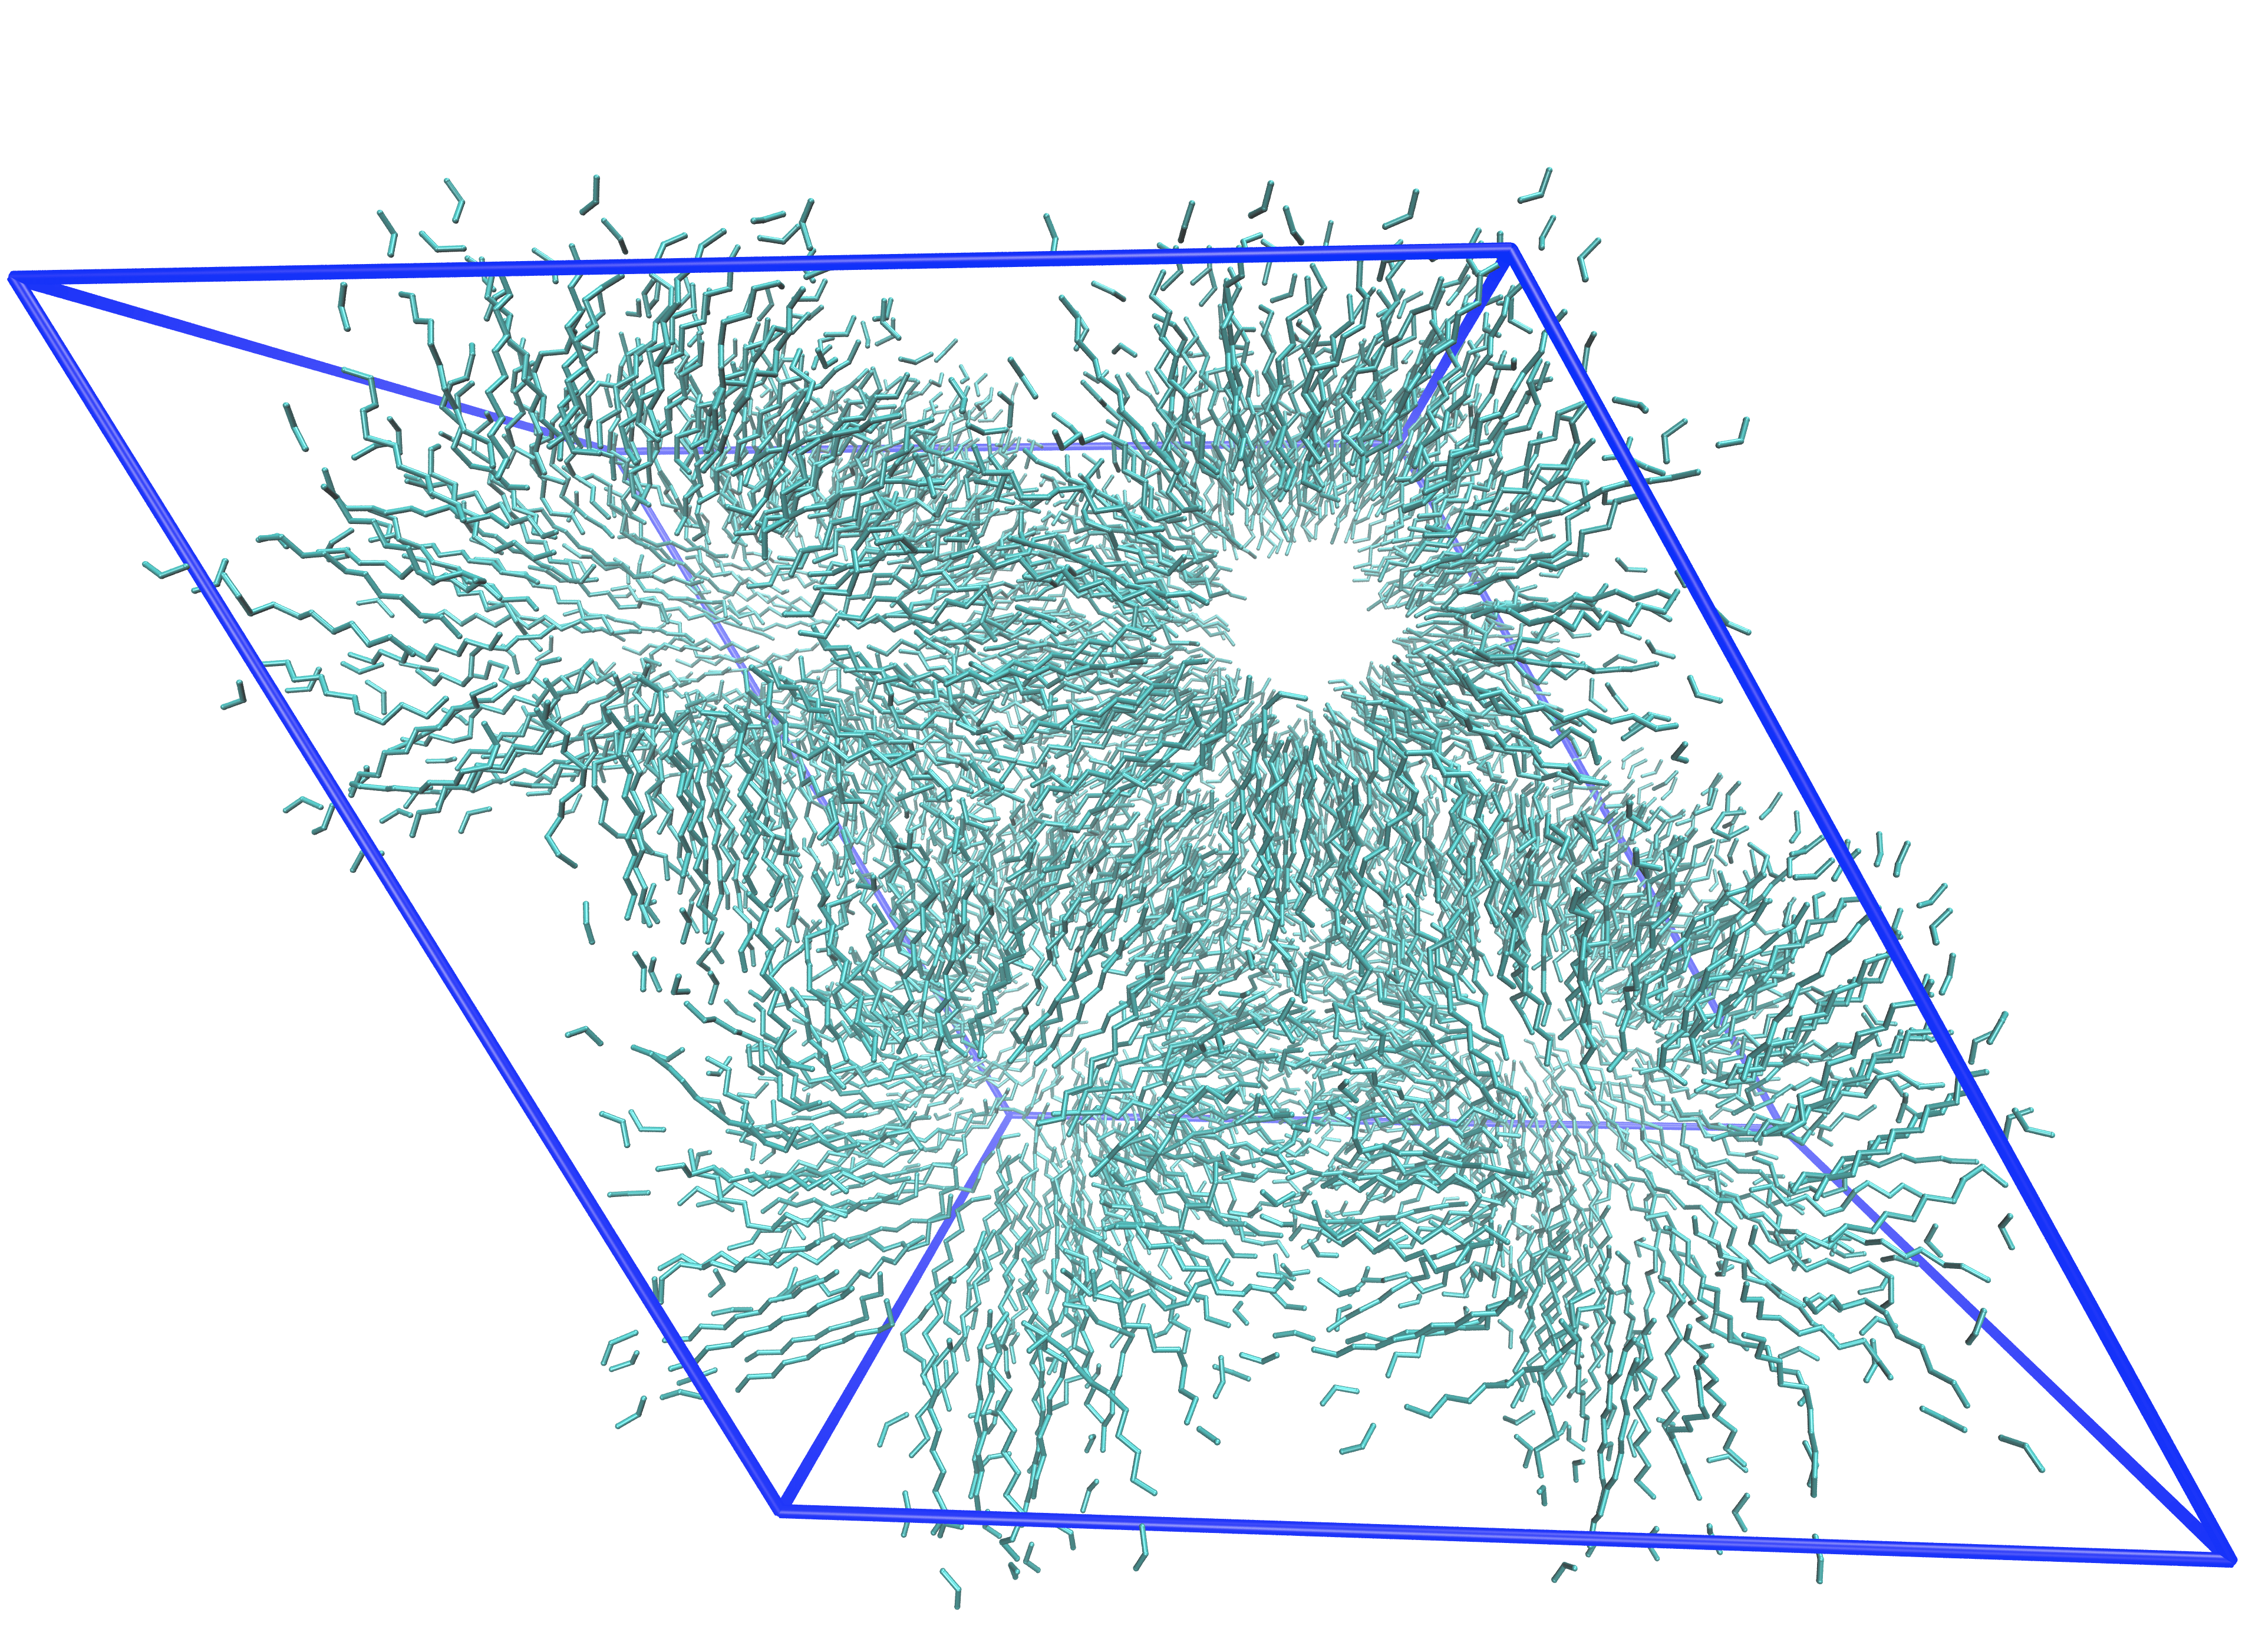
\includegraphics[width=\textwidth]{tails_topview.png}  % picture of top of unit cell with only tail atoms shown
		\caption{}\label{fig:topdown_tails_only}
	\end{subfigure}
	\begin{subfigure}{0.45\linewidth}
		\centering
		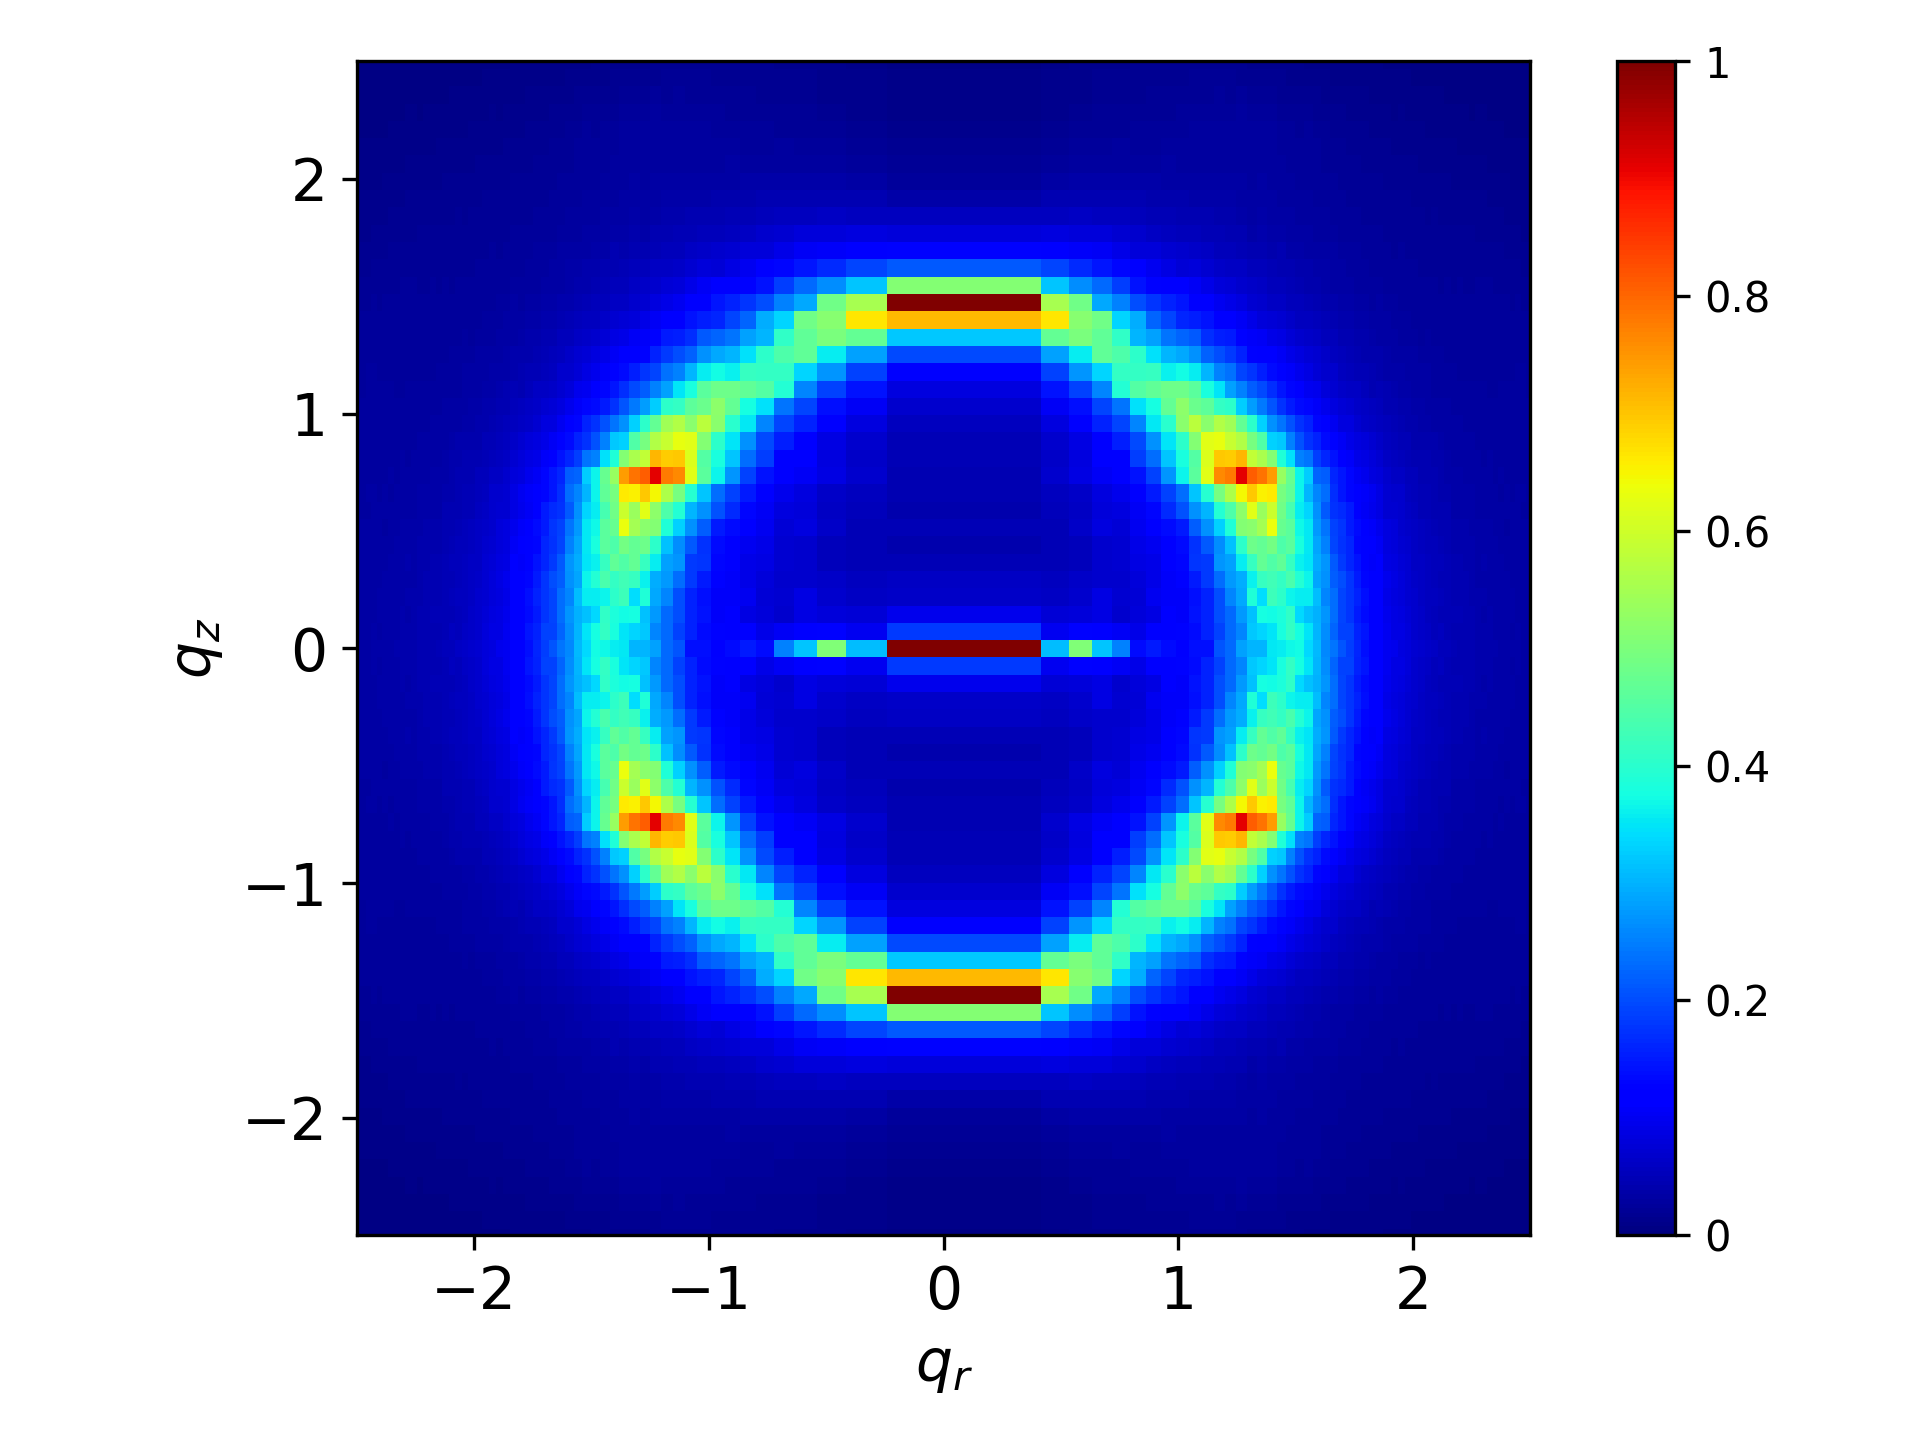
\includegraphics[width=\textwidth]{tails_rzplot.png}
		\caption{}\label{fig:tails_rzplot}
	\end{subfigure}
	\caption{(a) All atoms except carbon atoms making up the tails are removed from a 
	sandwiched configuration trajectory. (b) The simulated diffraction pattern of the
        tail-only trajectory still shows R-spots}\label{fig:tails}
  \end{figure}

  \begin{figure}[!htb]
  \centering
  	\begin{subfigure}{\linewidth}
	\centering
		\begin{subfigure}{0.45\textwidth}
        		\centering
        		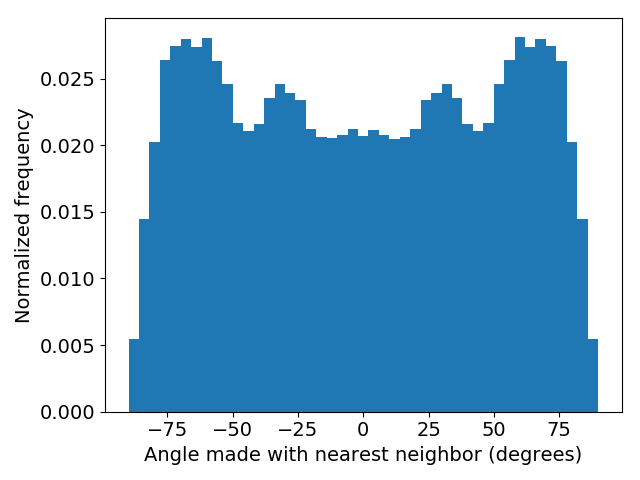
\includegraphics[width=\linewidth]{offset_tail_packing.png}
        		\caption{}~\label{fig:offset_tails}
		\end{subfigure}
		\begin{subfigure}{0.45\textwidth}
		\centering
	        	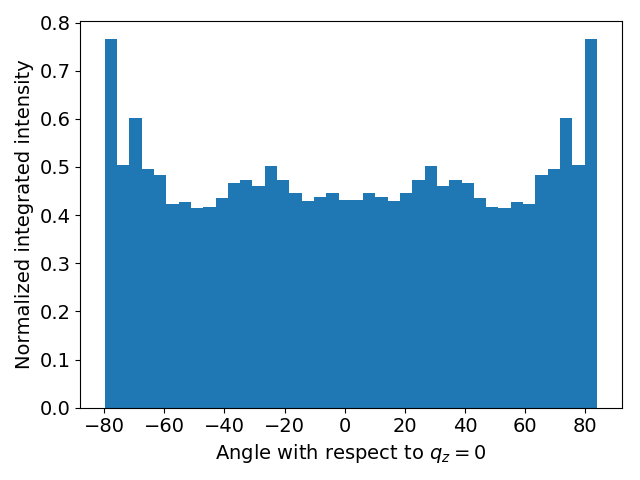
\includegraphics[width=\linewidth]{offset_angle_v_I.png}
		        \caption{}~\label{fig:offset_integration}
		\end{subfigure}
	\end{subfigure}
	\begin{subfigure}{\linewidth}
	\centering
		\begin{subfigure}{0.45\textwidth}
	        \centering
		        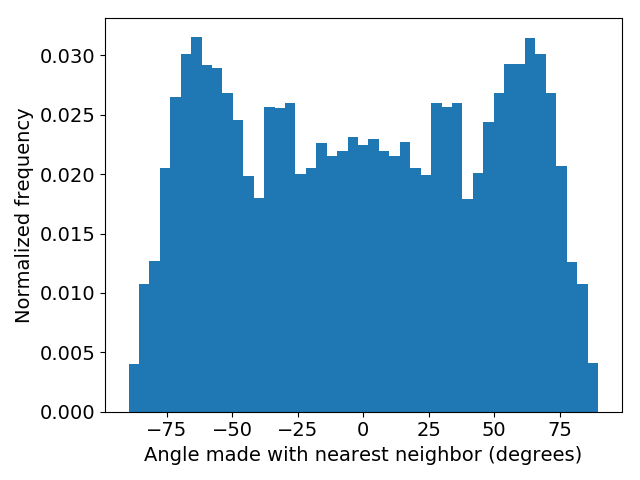
\includegraphics[width=\linewidth]{angles_traj_layered.png}
		        \caption{}~\label{fig:layered_tails}
		\end{subfigure}
		\begin{subfigure}{0.45\textwidth}
        	\centering
		        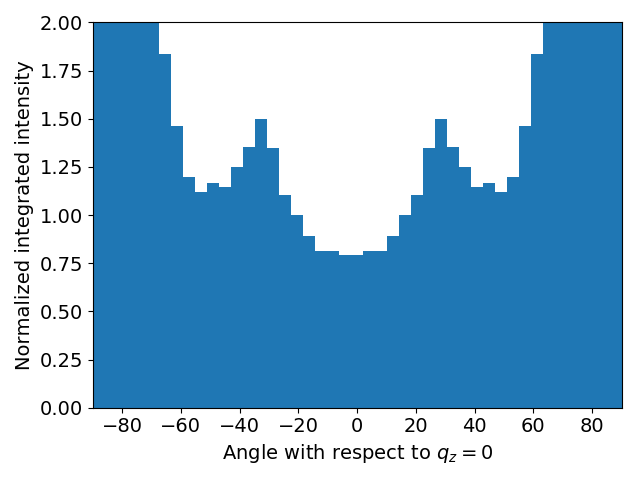
\includegraphics[width=\linewidth]{layered_angle_v_I.png}
		        \caption{}~\label{fig:layered_integration}
		\end{subfigure}
	\end{subfigure} 
  \caption{The distribution of angles w.r.t. the xy plane between alkane chain tail centroids and nearest
  neighbor centroids for equilibrated parallel displaced (a) and sandwiched (c) configurations. The
  same peaks are visible when the 2D simulated diffraction data is radially integrated in the R-alkanes region,
  (b) and (d) respectively.}~\label{fig:tail_packing}
  \end{figure}

  \subsection{Initial Layer Spacing Affects System Equilibration}

%  The $z$-direction correlation functions show that layers in our model prefer
%  to stack further apart than 3.7 \angstrom as suggested by experiment.
  When systems are built with layers stacked 5.0 \AA~apart then
  equilibrated, we observe long-term stability of a qualitatively different
  configuration suggesting that we have found another metastable free energy
  basin, further corroborating (\ref{point:metastable}). We studied this type of
  system in both the parallel displaced and sandwiched configurations. 

  Structural properties are different when layers are initially spaced 5 \AA~
  apart. In both configurations, we observe a decrease in pore spacing
  (Fig.~\ref{fig:p2p_disordered}) and a corresponding increase in the equilibrated
  distance between layers (Fig.~\ref{fig:dbwl_disordered}). The simulated X-ray
  diffraction patterns indicate further structural differences. In the parallel
  displaced configuration, almost all contrast between R-spots and R-alkanes is faded
  (Fig. ~\ref{fig:offset_disordered_xrd}). In the sandwiched
  configuration, R-spots is weakly present, but in different locations, showing higher
  intensity at the top and bottom of the pattern as well as at the intersection
  of R-alkanes with q$_z$ = 0 (Fig. ~\ref{fig:layered_disordered_xrd}). 

  Neither assembly deviates from its initial head group arrangement. R-helix is still 
  faintly visible in the parallel displaced configuration and is absent in the 
  sandwiched simulated diffraction pattern. The spectroscopic signatures are unique to
  the two different head group configurations.

  \begin{figure}[!hbt]
        \centering
        \begin{subfigure}{0.45\linewidth}
                \centering
                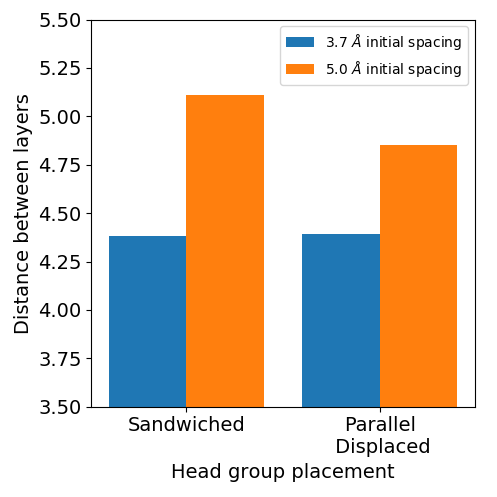
\includegraphics[width=\linewidth]{dbwl.png}
                \caption{}~\label{fig:dbwl_disordered}
        \end{subfigure}%
        \begin{subfigure}{0.45\linewidth}
                \centering
                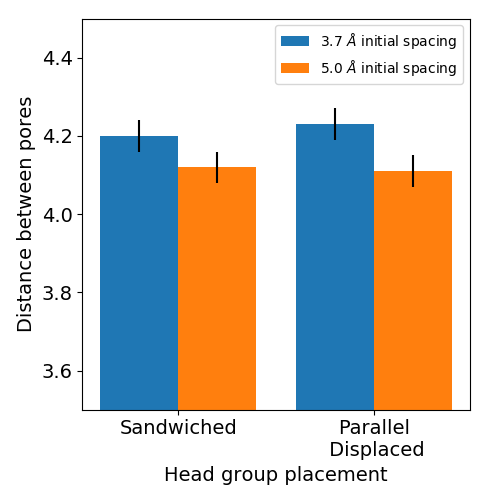
\includegraphics[width=\linewidth]{p2p2.png}
                \caption{}~\label{fig:p2p_disordered}
        \end{subfigure}
        \begin{subfigure}{0.45\linewidth}
                \centering
                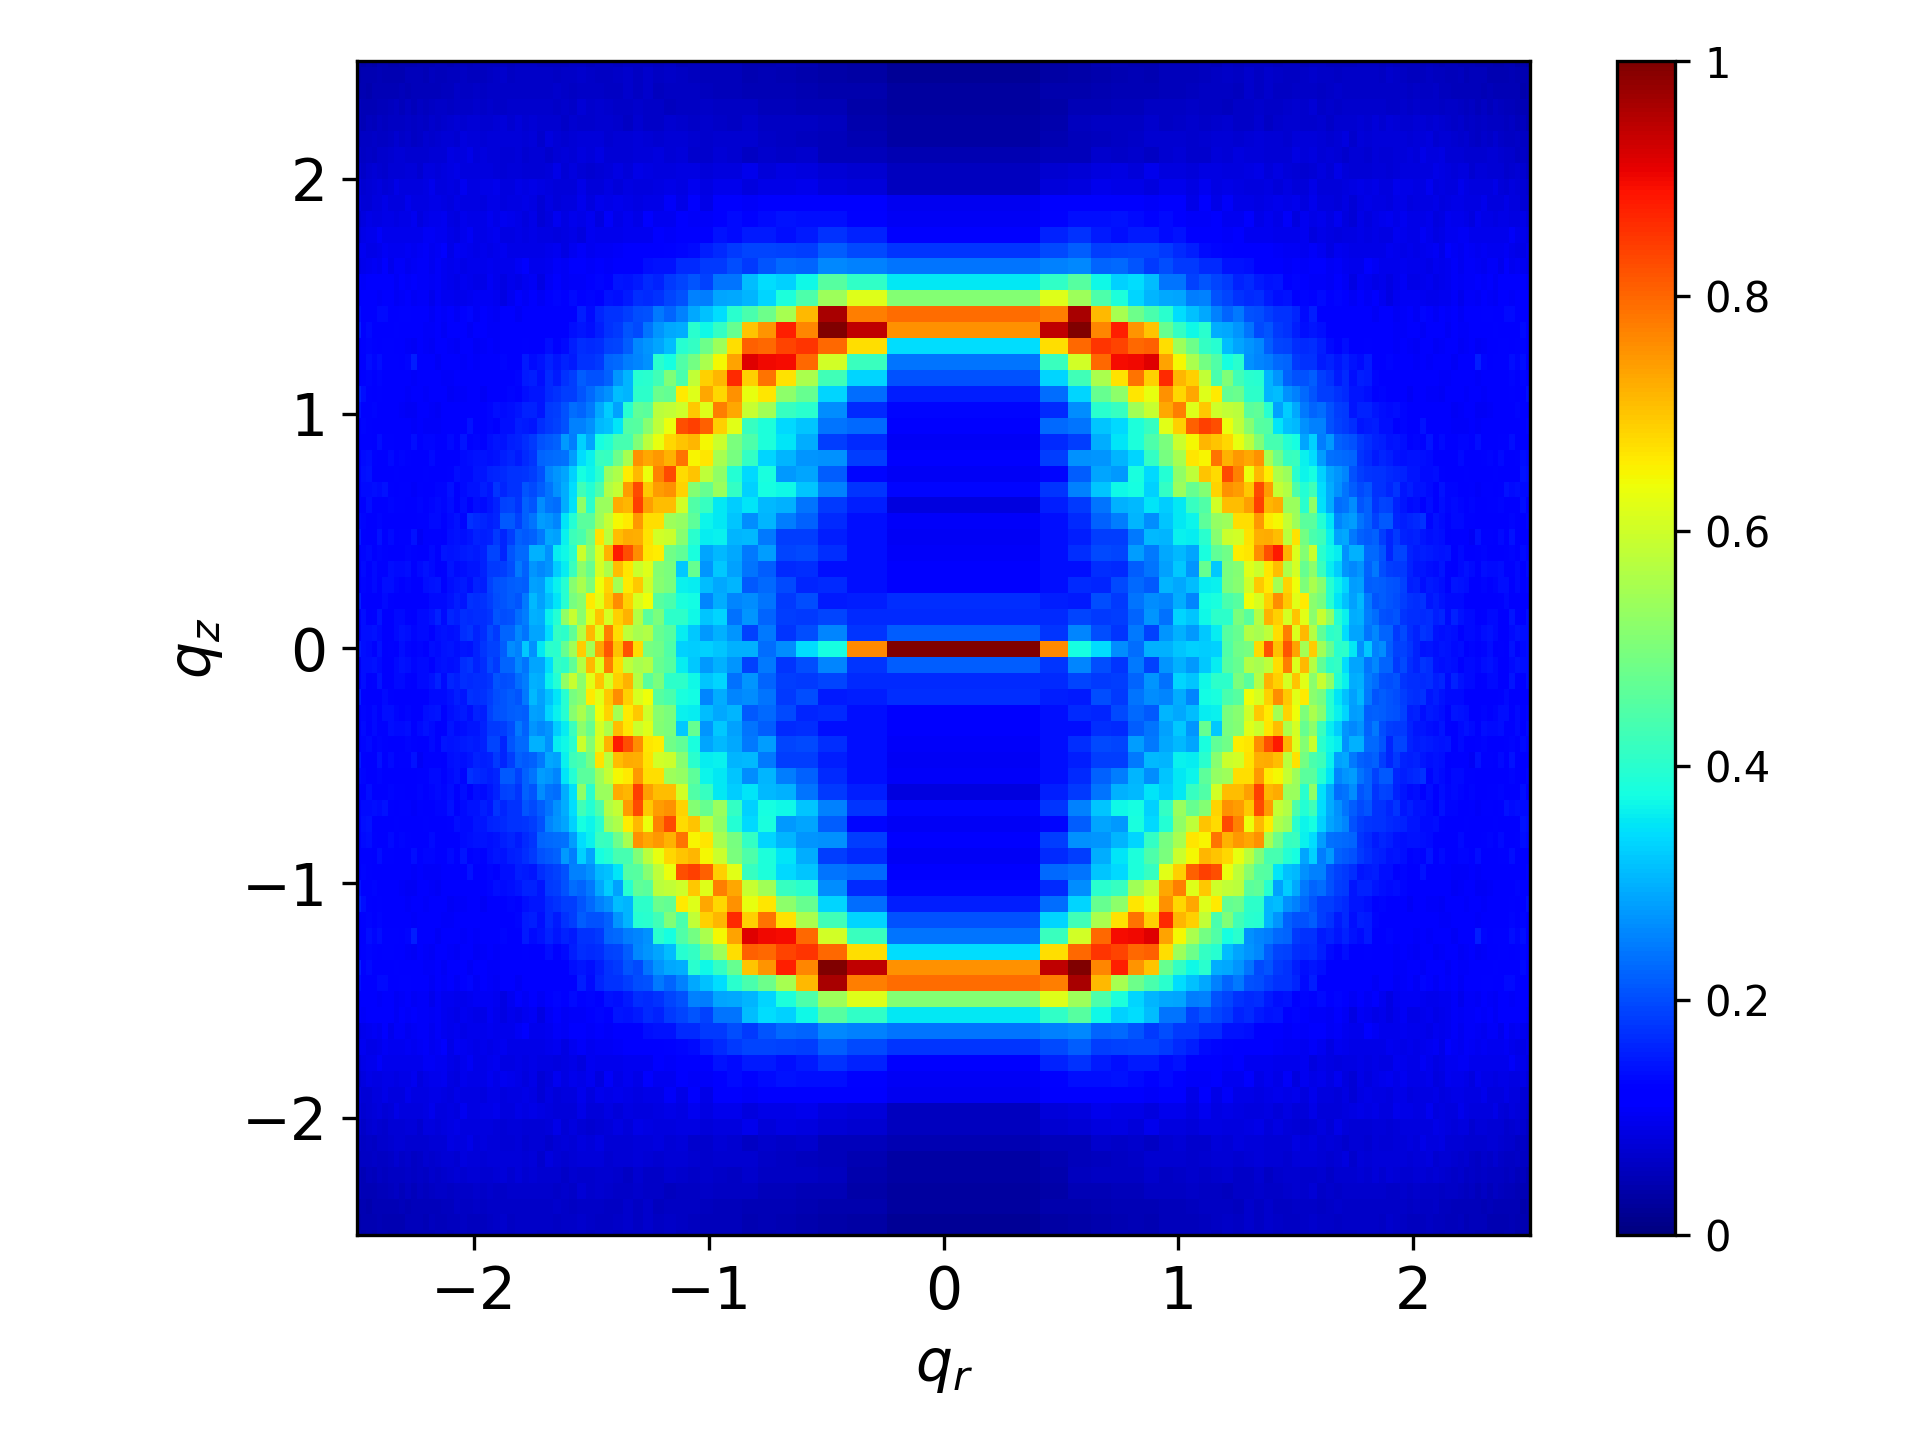
\includegraphics[width=\linewidth]{offset_disordered_rzplot.png}
                \caption{}~\label{fig:offset_disordered_xrd}
        \end{subfigure}%
        \begin{subfigure}{0.45\linewidth}
                \centering
                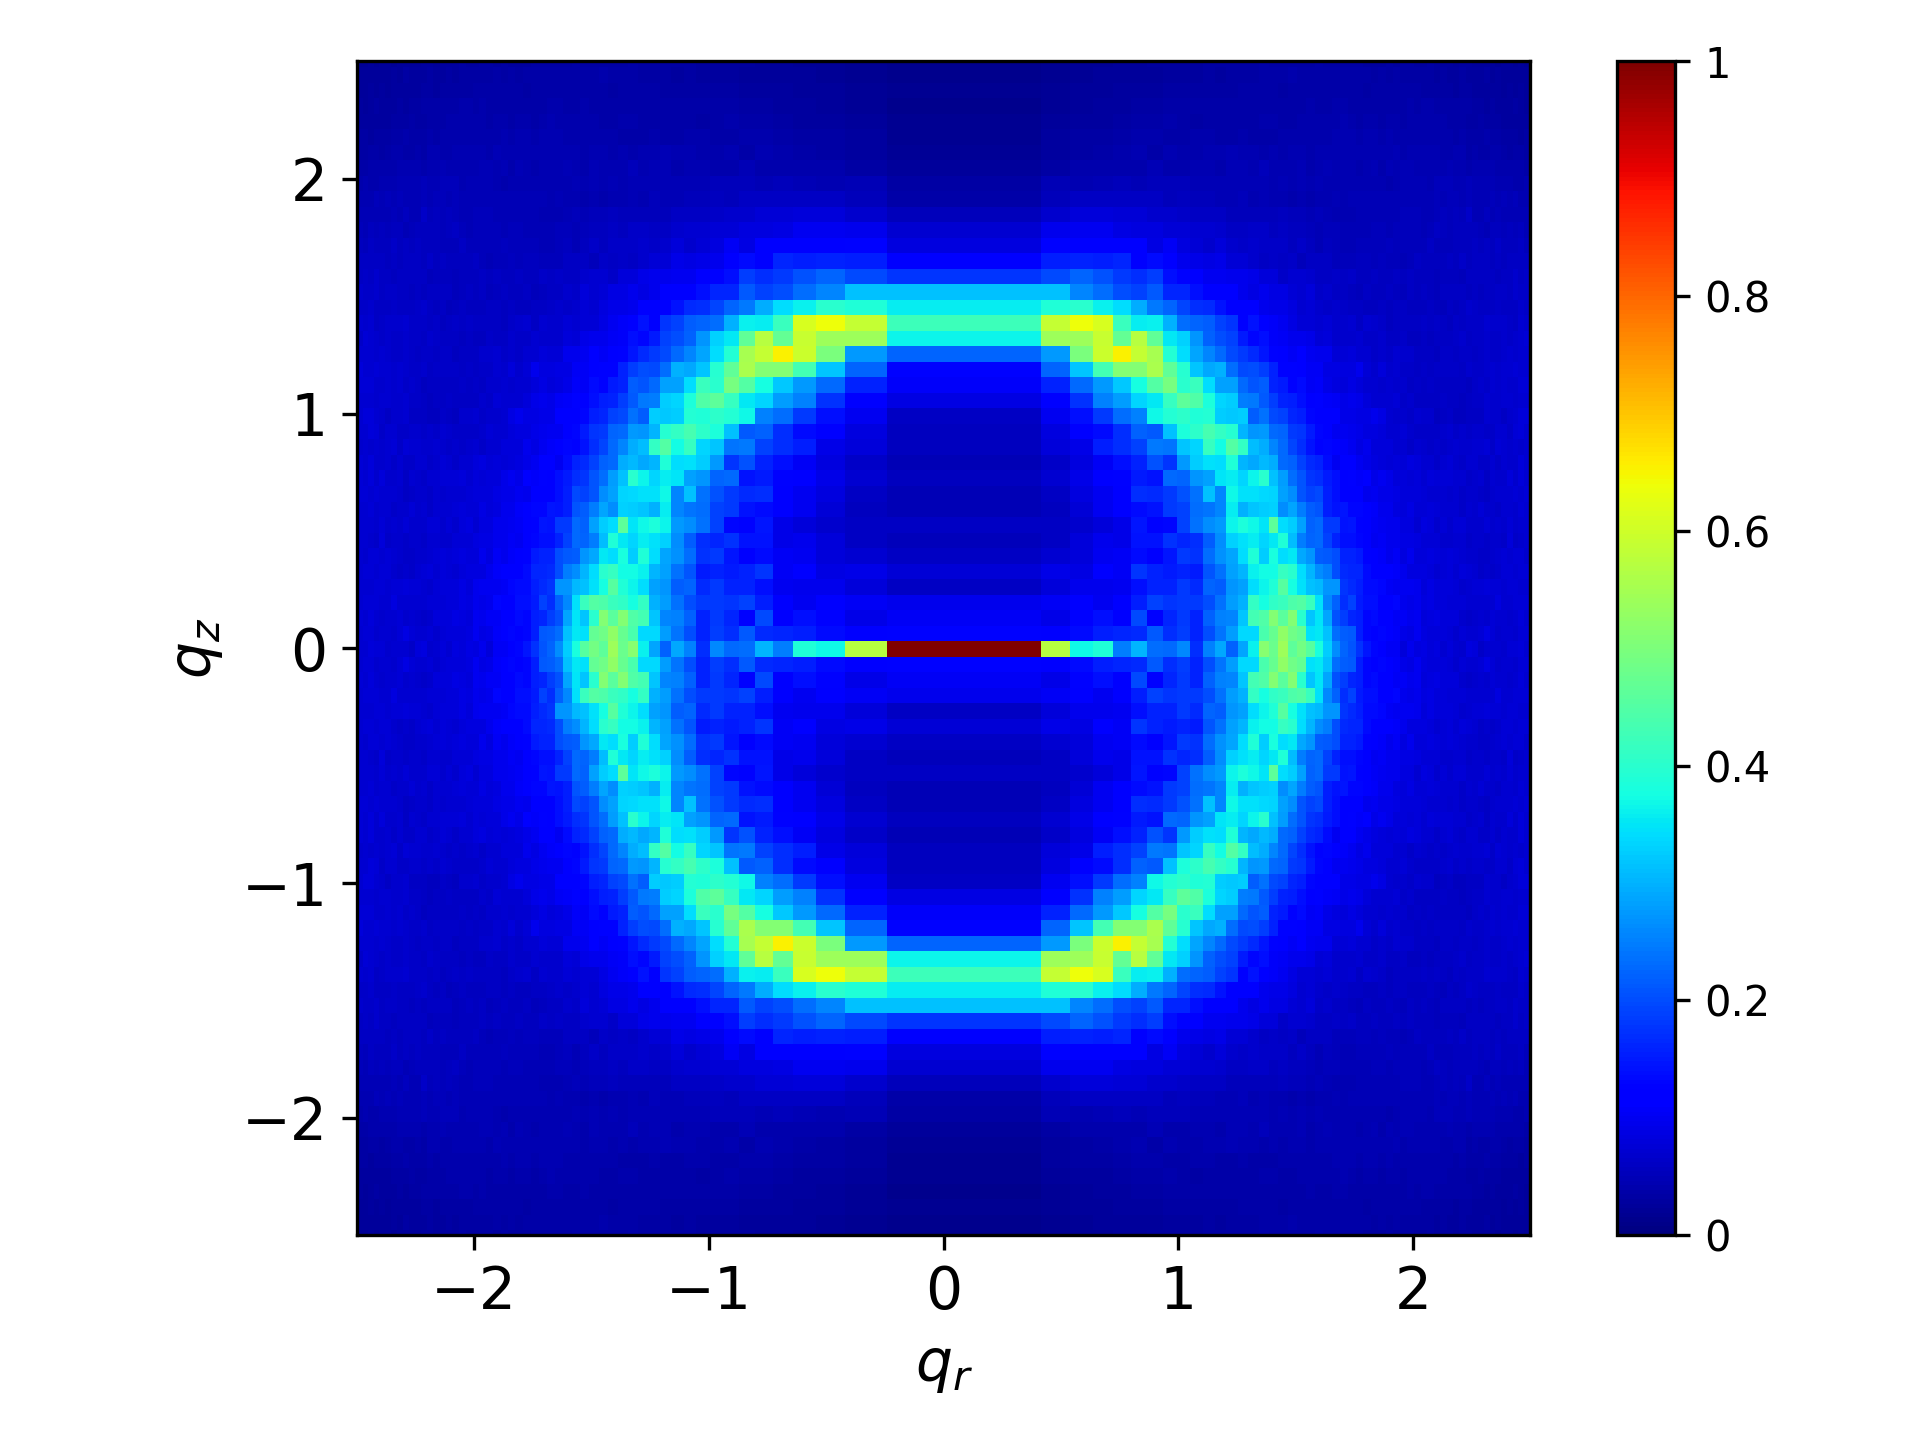
\includegraphics[width=\linewidth]{layered_disordered_rzplot.png}
                \caption{}~\label{fig:layered_disordered_xrd}
        \end{subfigure}
	\caption{In comparison to systems built with 3.7 \AA~ initial layer spacing,  
                the simulated X-ray diffraction patterns of the parrallel displaced (a) and 
 		sandwiched (b) configurations are different when systems are built with 
 		a 5 \AA~ initial layer spacing, most notably in the region bounded by R-alkanes.
      		When layers are stacked further apart, the distance between layers increases (c)
                and the pore spacing decreases (d).}
  \end{figure}

  \subsection{Pore Structure Depends on Initial Configuration}

  In order to address (\ref{point:poredefinition}), we plotted the number of
  densities of heavy atoms in the head group, carbon atoms in the tail region
  and the sodium ions (Figure~\ref{fig:densities}). For the head group region,
  we used the carbon atoms making up the aromatic ring. For the tail region we
  used only carbon atoms of the monomer tails (See Supplemental Information for
  diagram). Histograms are averaged over at least 50 ns of equilibrated trajectory.

  In all cases, the space in the pore region is filled with sodium ions and
  head groups. There is a clear partition between the hydrophobic and hydrophilic
  regions. Alkane tails do not cross into the pore region. We expect that when 
  water is introduced to the system, water molecules will occupy the hydrophilic region
  and open up the pores for aqueous solute transport. 

  The sandwiched configuration (Fig. \ref{fig:layered_density}) shows a relatively
  ordered pore structure. The number densities of components in all other
  configurations are comparable. In contrast, sodium ions and head groups in the
  sandwiched configuration are highly concentrated away from the pore center
  meaning that there is vacancy in the pore region. A vacant pore is very likely
  to be unstable in a real system, further supporting the physical realism of the
  parallel displaced configuration. 

  % BJC: TODO: Increase font size
  %            Put insets in the figures that make it clear what configuration each represents
  \begin{figure}
  \centering
  \begin{subfigure}{0.45\textwidth}
        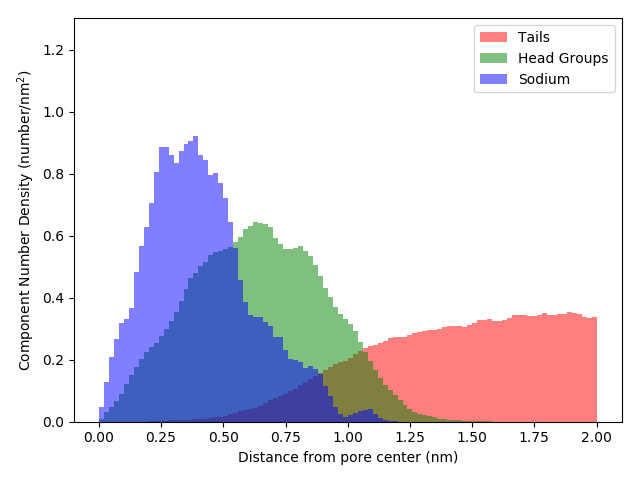
\includegraphics[width=1\linewidth]{offset_density.png}
        \caption{}
        \label{fig:offset_density}
  \end{subfigure}
  \begin{subfigure}{0.45\textwidth}
        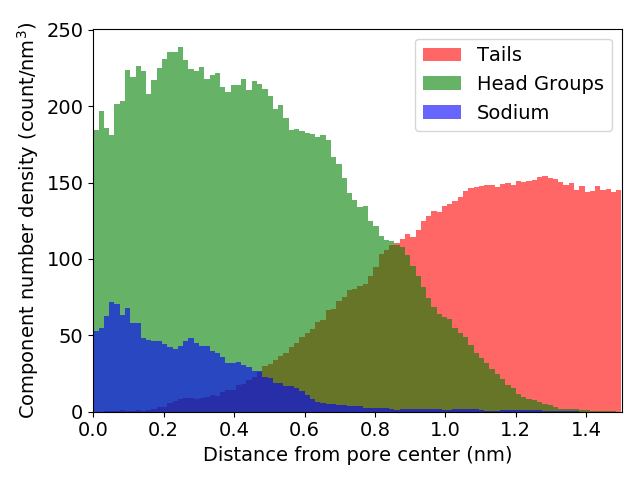
\includegraphics[width=1\linewidth]{layered_density.png}
        \caption{}
        \label{fig:layered_density}
  \end{subfigure}
  \begin{subfigure}{0.45\textwidth}
        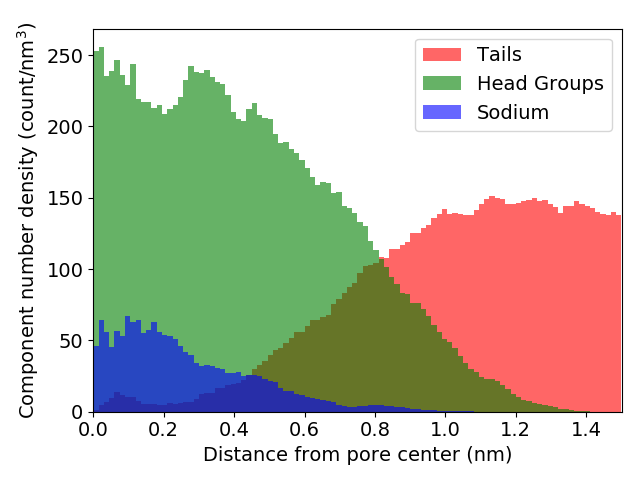
\includegraphics[width=1\linewidth]{disordered_offset_density.png}
        \caption{}
        \label{fig:disordered_offset_density}
  \end{subfigure}
  \begin{subfigure}{0.45\textwidth}
        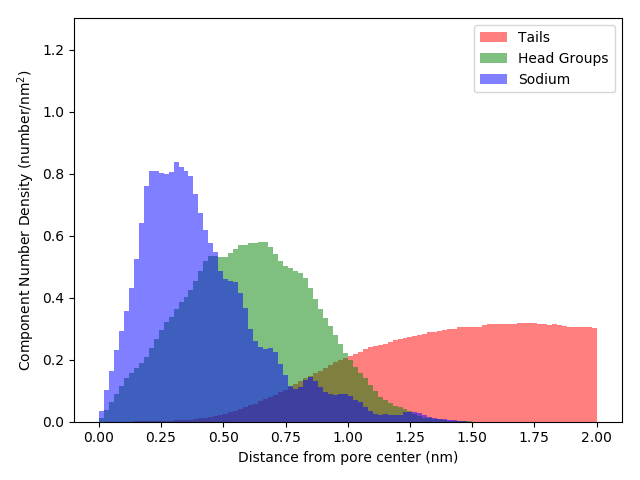
\includegraphics[width=1\linewidth]{disordered_density.png}
        \caption{}
        \label{fig:disorder_layered_density}
  \end{subfigure}
  \caption{In all cases, assemblies stay partitioned into hydrophilic and
	  hydrophobic regions. The parallel displaced (a), the disordered parallel
	  displaced (c), and the disordered sandwiched (d) show similar pore structures.
	  The sandwiched configuration (b) exhibits an open pore structure with sodium
	  ions and head groups concentrated away from the pore
	  center.}~\label{fig:densities}
  \end{figure}

  \subsection{Affect of Water on Structure}

  % BJC: Is it necessary to show layered configurations at this point?
  We answered (\ref{point:water}) and further support (\ref{point:orientation})
  by preparing parallel displaced and sandwiched configurations according to the
  wet equilibration procedure. There is no experimental measurement of trace
  water concentration in the pores so we tested a range of water concentrations
  from 0.5 to 5 percent. Our lower bound models a system with on average 2 water
  molecules for each monomer layer. Figure ~\ref{fig:solvation} shows the
  simulated diffraction patterns resulting from each configuration.

  % BJC: TODO: reformat
  %            adjust colorbar
  \begin{figure}
	\centering
	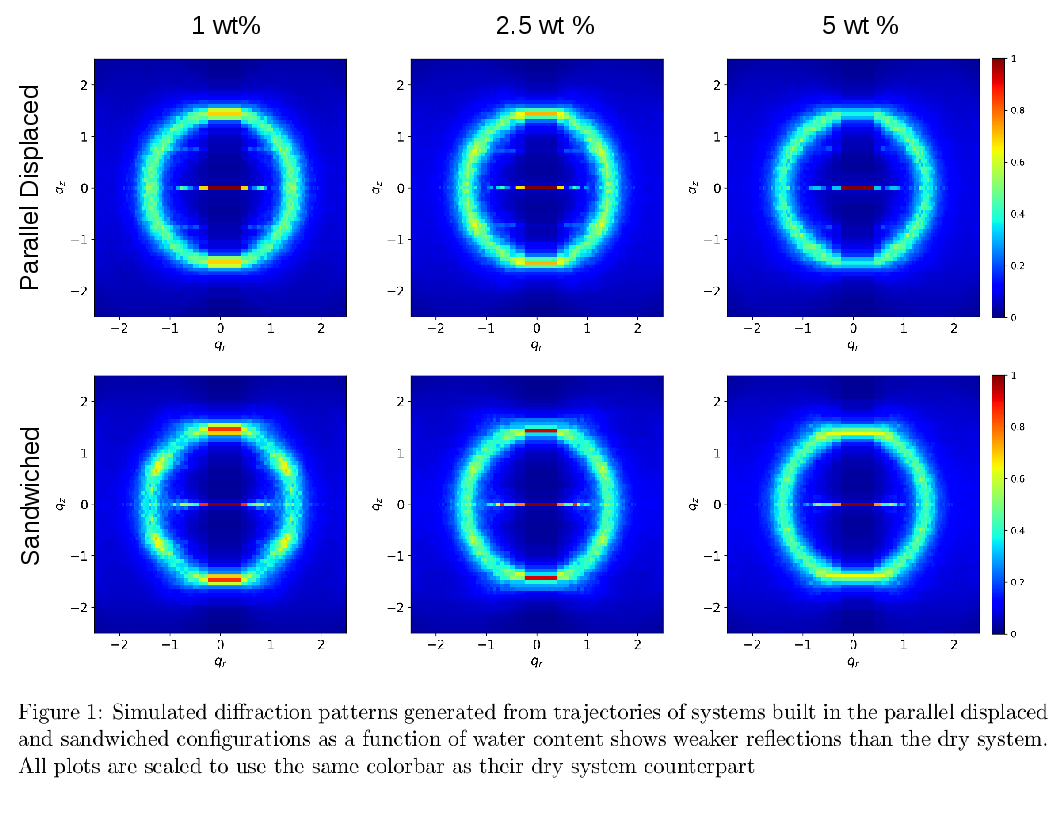
\includegraphics[width=\textwidth]{solvation.png}  % still working on formatting so this is a screenshot of a doctored latex figure
        %MRS2: include 0% as well? Maybe leave off 5% if not relevant in the end?
	\caption{}
	\label{fig:solvation}
  \end{figure}

  In all cases, water disrupts structuring of the model. The plots in Figure
  ~\ref{fig:solvation} are normalized to have the same colorbar as the dry
  systems. The intensity of the reflections decrease when water is added to the
  system. In systems built with 5 wt \% water, R-$\pi$ and R-spots
  become nearly indistinguishable from R-alkanes.

  % BJC: unsure where or if this paragraph fits
  Water is not necessary to maintain an ordered pore structure. We do not
  eliminate the possibility that water is necessary in order to drive
  self-assembly, however, studying the mechanisms of self assembly is beyond the
  scope of this work. According to our model, once the system has formed the
  Col\textsubscript{h} phase, adding water only drives disorder of the pore
  structure. In the true equilibrium configuration, if water exists, it is
  primarily confined to the pore region where there is no driving force for
  aggregation of water molecules. In the case of trace water, water molecules
  will be too sparse to form a hydrogen bonding network.

  In systems built with 5 wt~\% water, the pore region becomes filled with
  water. We plotted the number density of components in this system and see that
  the pores become a soup of water molecules and sodium ions (Fig.
  \ref{fig:water_density}). This system is a closer representation of the
  H\textsubscript{II} phase which is typically synthesized with ca. 8 wt \%
  water. We believe that the hydrated membrane pores will be valuable for aqueous
  separations. Further analysis of and transport within the H\textsubscript{II}
  phase are left for future studies.

  %BJC: TODO: Bigger fonts
  \begin{figure}
  \centering 
  \begin{subfigure}{0.45\textwidth}
        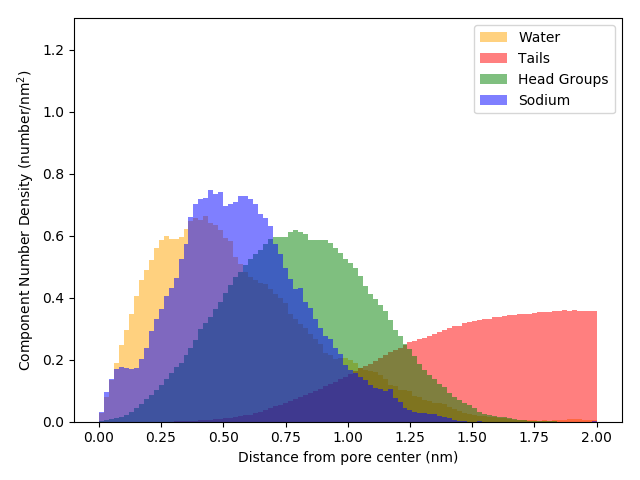
\includegraphics[width=1\linewidth]{offset_solvated_density.png}
        \caption{}
        \label{fig:offset_solvated_density}
  \end{subfigure}
  \begin{subfigure}{0.45\textwidth}
        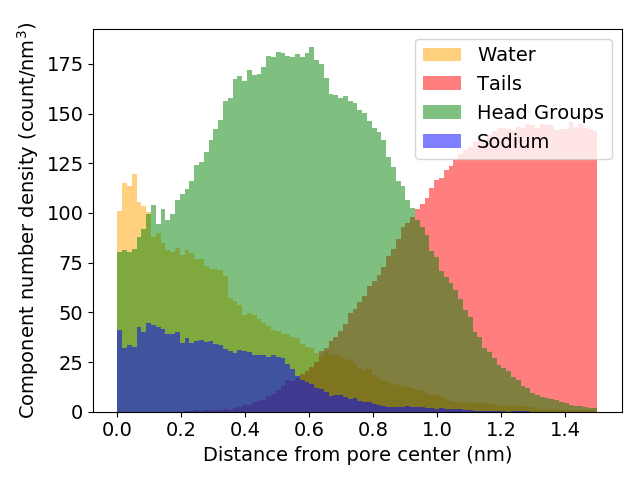
\includegraphics[width=1\linewidth]{layered_solvated_density.png}
        \caption{}
        \label{fig:layered__solvated_density}
  \end{subfigure}
  \caption{Water fills the membrane pores in the parallel displaced (a) and 
  sandwiched (b) configurations. Sodium ions are distributed more uniformly 
  in the sandwiched configuration.}
  \label{fig:water_density}
  \end{figure}

  \subsection{Model Ionic Conductivity Measurements}

  We used the equilibrated parallel displaced system to calculate ionic
  conductivity since its structure is the closest match to experiment. The model
  gives reasonable estimates of ionic conductivity when compared to experiment.
  Calculated values of ionic conductivity obtained using the Nernst-Einstein
  relation and Collective Diffusion model are compared in
  Figure~\ref{fig:conductivity}. The two methods agree with each other within
  error, although the uncertainty obtained using the Collective Diffusion model
  is much higher. Much longer simulations are needed to lower the uncertainty,
  however it is not feasible to do so with a large system. We will only use the
  Nernst-Einstein relation in future calculations of this type. 

  The calculated values of ionic conductivity are higher than experiment by an
  order of magnitude. One can justify the reason for this result by considering
  the real system studied experimentally. The ionic conductivity measurement to
  which we are comparing was done on a \SI{80}{\micro\metre} thick film, nearly
  10,000 times thicker than our simulated system. The thick film likely has
  defects leading to non-contiguous pores and imperfect alignment.  It has been
  shown that there is a large dependence of ionic conductivity on the alignment
  of the pores. The ionic conductivity of an unaligned film is ca. 85 times lower
  than that of a nearly aligned film referenced here. We hypothesize that a thin,
  perfectly aligned film would have a value of ionic conductivity in close 
  agreement with our model.
 
  \begin{figure}
        \centering
        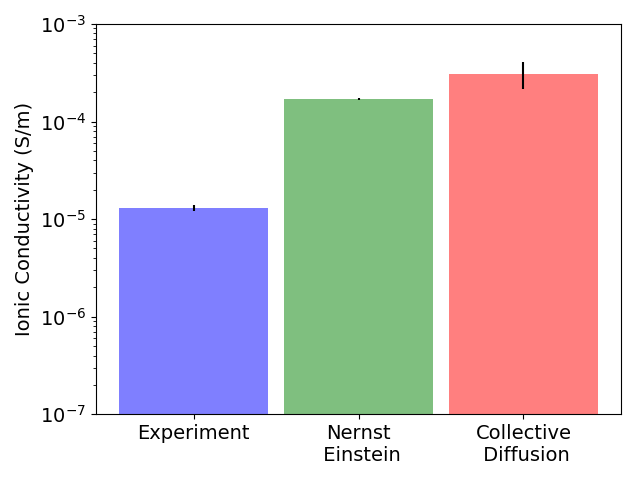
\includegraphics[width=0.5\linewidth]{IC_offset.png}
        \caption{Calculated ionic conductivity using the Nernst-Einstein relation
        and Collective Diffusion model agree with error. Both methods give calculated
        values of ionic conductivity an order of magnitude higher than the experimental
        value.}
        \label{fig:conductivity}
  \end{figure}

  \subsection{Affect of Crosslinking}\label{section:xlink}

  The system's structure and physical characteristics did not change
  significantly when we applied the crosslinking algorithm to the equilibrated
  parallel-displaced configuration built with 5 monomers per layer. We simulated
  the crosslinked system in the NPT ensemble for 100 ns. The distance between
  pores shrinks by 0.4 \angstrom~ and the distance between layers increases by
  0.04 \AA~ after the system is crosslinked. All major features are still present
  in the simulated XRD patterns, however at lower intensities
  (Fig.~\ref{fig:rzplot_xlink}). We calculated the ionic conductivity using the
  Nernst-Einstein relation and found that it is lower in the crosslinked system
  (Fig.~\ref{fig:IC_xlink}).

  %BJC: add units
  \begin{figure}
  \centering
  \begin{subfigure}{0.45\textwidth}
	\centering
	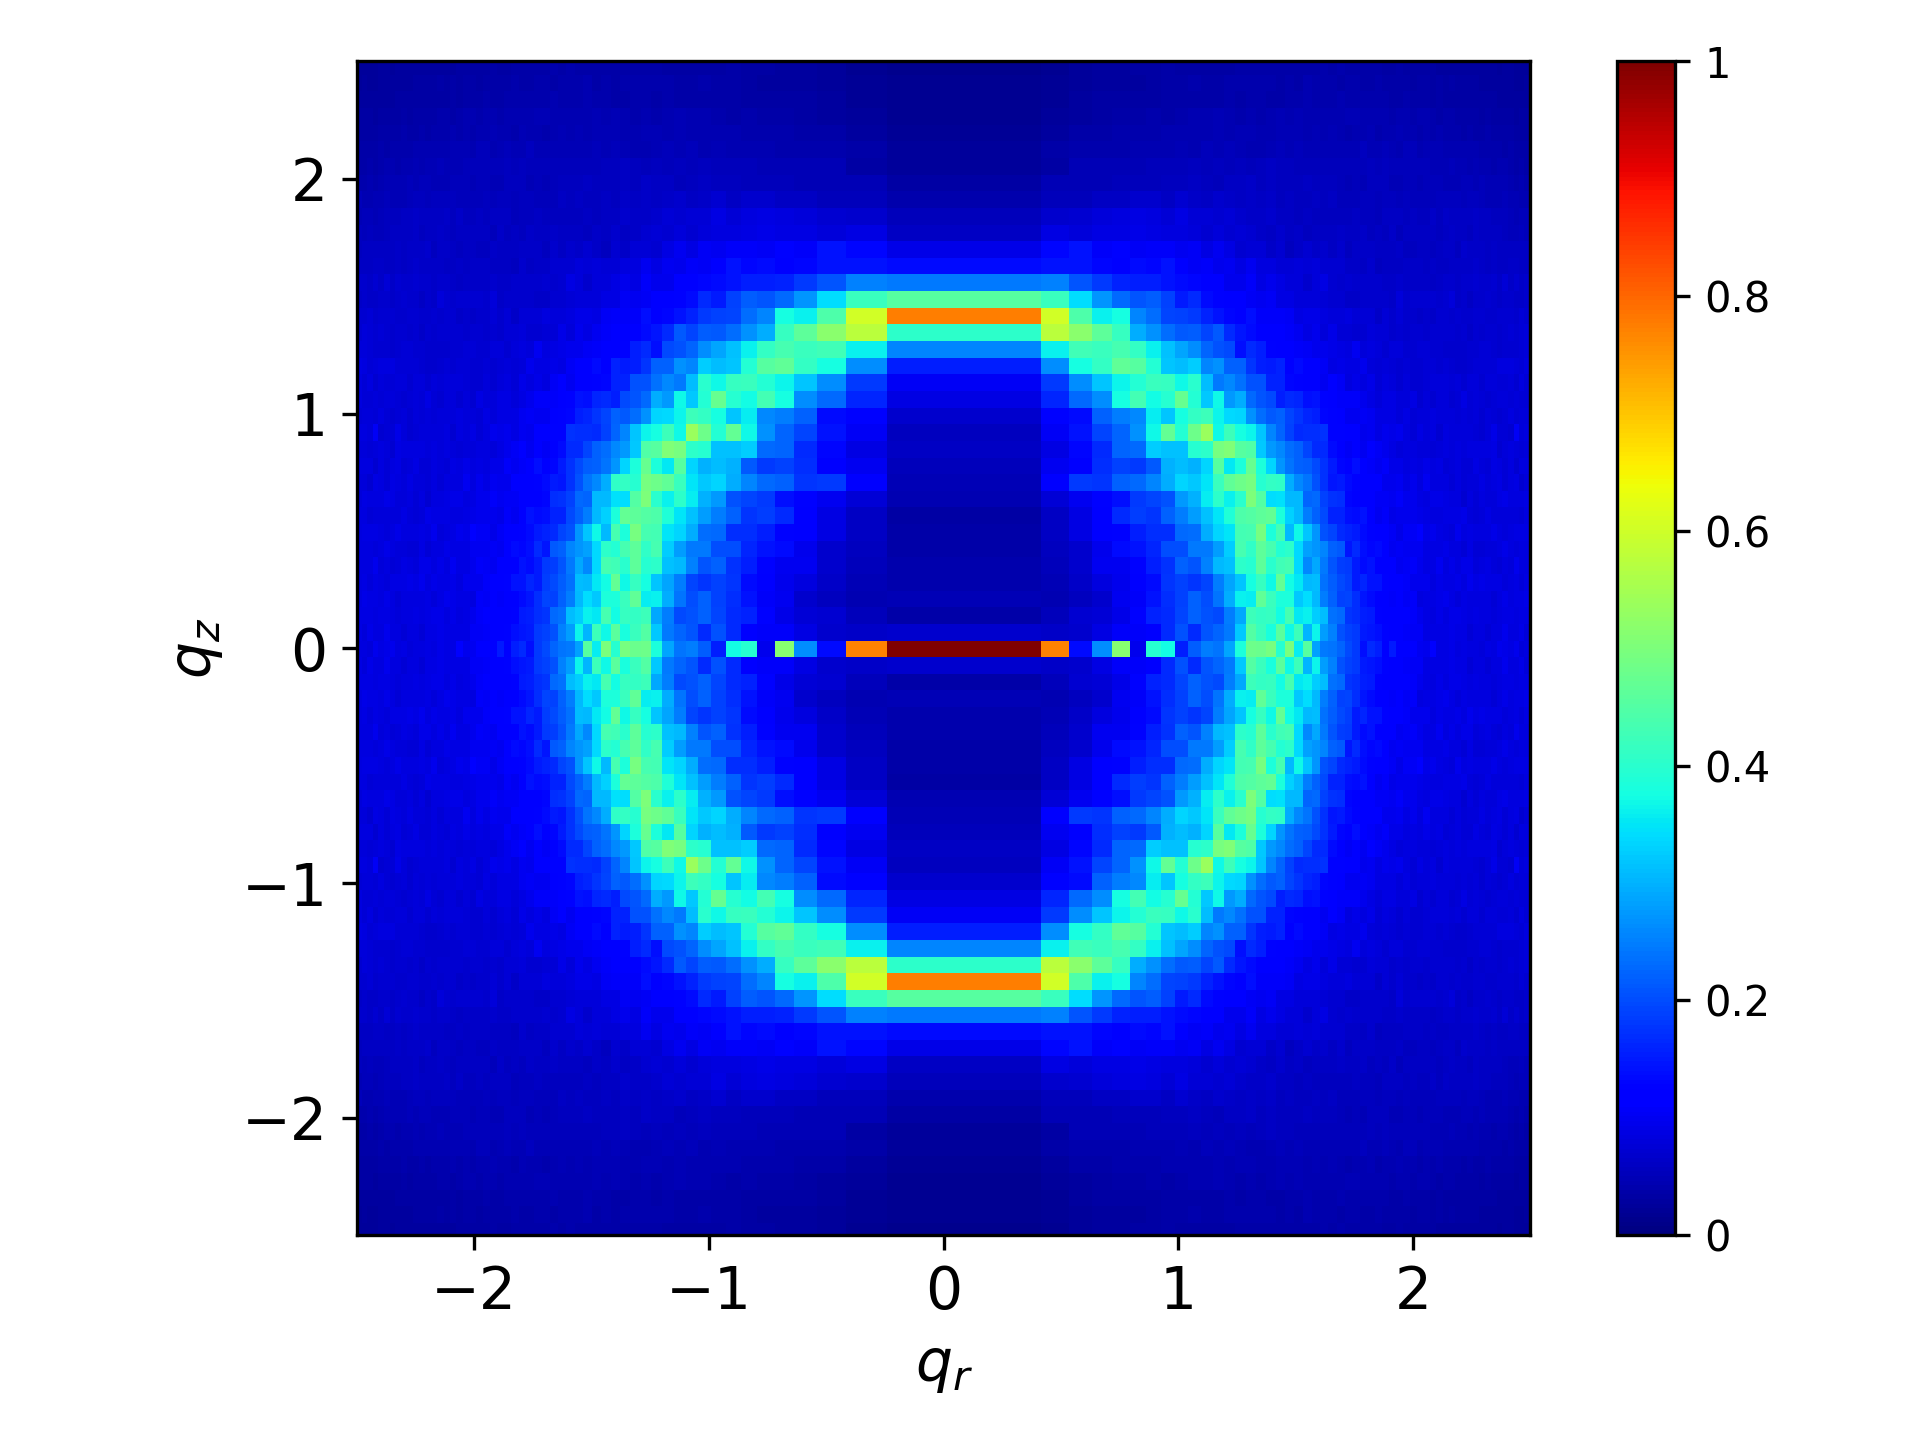
\includegraphics[width=\textwidth]{rzplot_xlink.png}
	\caption{}~\label{fig:rzplot_xlink}
  \end{subfigure}
  \begin{subfigure}{0.45\textwidth}
	\centering
	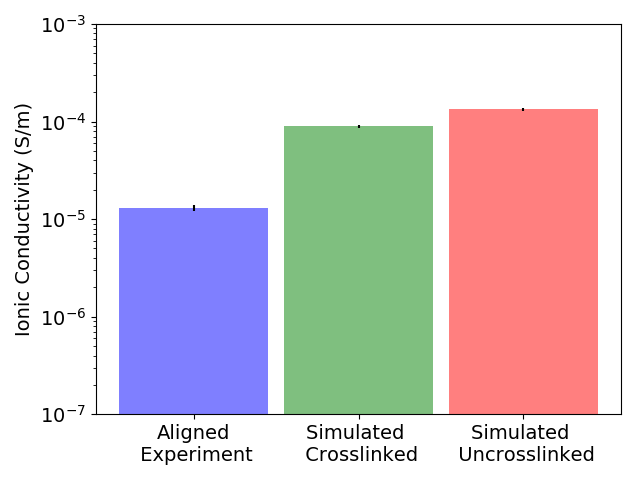
\includegraphics[width=\textwidth]{IC_xlink.png}
	\caption{}~\label{fig:IC_xlink}
  \end{subfigure}
  \begin{subfigure}{0.45\textwidth}
	\centering
	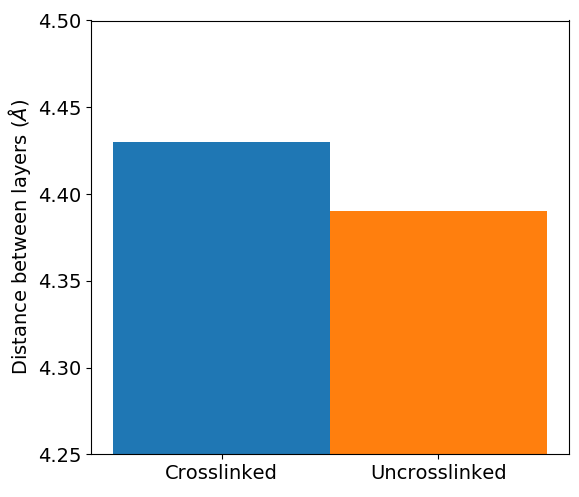
\includegraphics[width=\textwidth]{dbwl_xlink.png}
	\caption{}~\label{fig:dbwl_xlink}
  \end{subfigure}
  \begin{subfigure}{0.45\textwidth}
	\centering
	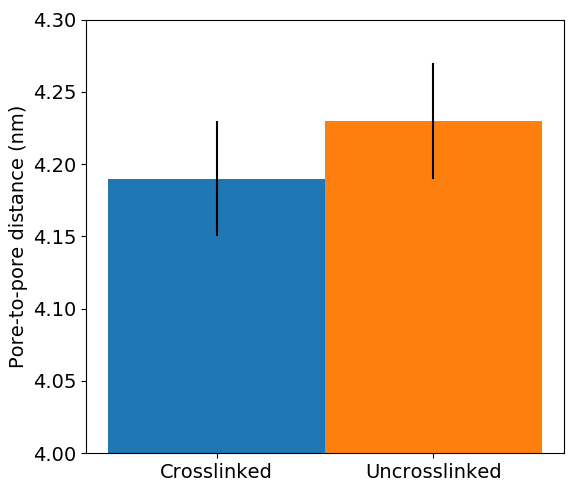
\includegraphics[width=\textwidth]{p2p_xlink.png}
	\caption{}~\label{fig:p2p_xlink}
  \end{subfigure}
  \caption{(a) Reflections produced by the crosslinked configuration fade relative
  to the uncrosslinked system. The colorbar shown is the same used for the uncrosslinked
  system. (b) The ionic conductivity is smaller relative to the uncrosslinked system, but
  still much larger than the experimental value. (c) The distance between layers increases
  when the system is crosslinked. (d) The pore spacing decreases when the membrane is 
  crosslinked.}~\label{fig:xlink}
  \end{figure}
 
  \section{Conclusion}
  
  % add stuff about pore structure and 'disordered' basin once there are concrete results 
  We have used a detailed molecular model of the Col\textsubscript{h} phase
  formed by Na-GA3C11 in order to study its nanoscopic structure. While there
  have been efforts to model formation of various liquid crystalline phases with
  molecular dynamics, to our knowledge there have been no studies which attempt
  to examine their structure with the same level of detail presented here.
  Evidence strongly supports that monomers stay partitioned into layers and that
  each layer contains 5 monomers. We have explored the affect of two different
  $\pi$-$\pi$ stacking modes on the equilibrated membrane strucure. Simulated
  diffration patterns generated from MD trajectories suggest that the
  parallel-displaced configuration produces a structure with the closest match to
  experiment. Finally, water is not needed to create well-definied pore
  structures. 

  Now that we have a good idea of what the membrane structure should
  look like, we will evaluate transport of various solutes within the system. We
  will apply the knowledge gained from this study in order to suggest
  improvements to the existing system as well as to evaluate new unsynthesized
  LLC systems.

  \clearpage
  \bibliography{llc}

\end{document}
